\documentclass[11pt]{article}

%PAKKER
\usepackage{booktabs}
\usepackage{amsmath, amssymb, amsthm, amsfonts}
\numberwithin{equation}{section}
\usepackage{fancyhdr}
\usepackage[margin=1.25in]{geometry}
\usepackage{datetime}
\usepackage{nicematrix}
\usepackage{enumitem}
\usepackage{commath}
\usepackage{calrsfs}
\usepackage{nameref}
\usepackage{hyperref}
\usepackage{listings}
\usepackage{color}
\usepackage{graphicx}
\usepackage{dsfont}
\usepackage{pgfplots}
\pgfplotsset{compat=newest}


\definecolor{codegreen}{rgb}{0,0.6,0}
\definecolor{codegray}{rgb}{0.5,0.5,0.5}
\definecolor{codepurple}{rgb}{0.58,0,0.82}
\definecolor{backcolour}{rgb}{0.95,0.95,0.92}

\lstdefinestyle{mystyle}{
    backgroundcolor=\color{backcolour},   
    commentstyle=\color{codegreen},
    keywordstyle=\color{magenta},
    numberstyle=\tiny\color{codegray},
    stringstyle=\color{codepurple},
    basicstyle=\ttfamily\footnotesize,
    breakatwhitespace=false,         
    breaklines=true,                 
    captionpos=b,                    
    keepspaces=true,                 
    numbers=left,                    
    numbersep=5pt,                  
    showspaces=false,                
    showstringspaces=false,
    showtabs=false,                  
    tabsize=2
}

\lstset{style=mystyle}
\newcommand{\indep}{\rotatebox[origin=c]{90}{$\models$}}
%QED SYMBOL
\renewcommand{\qedsymbol}{$\blacksquare$}
\def\code#1{\texttt{#1}}
%AFSNIT OG HEADHEIGHT
\setlength{\parindent}{0.5cm}
\setlength{\headheight}{15pt}
\DeclareMathAlphabet{\mathcal}{OMS}{cmsy}{m}{n}
\begin{document}
%SIDEHOVED OG -FOD
\pagestyle{fancy}
\fancyfoot{}
\fancyfoot[C]{\thepage}
\fancyhead[C]{}
\fancyhead[L]{}
\fancyhead[R]{}
\renewcommand{\headrulewidth}{0pt}
\renewcommand{\footrulewidth}{0pt}
\allowdisplaybreaks

%BIBTEX
\bibliographystyle{siam}

%TITEL
\title{Tipping Point Estimation in Ecological Systems using Stochastic Differential Equations}
\author{Anders G. Kristensen \\
Supervisor: Susanne Ditlevsen}
\date{31st of May, 2024}
\maketitle
\section*{Abstract}\label{Abstract}
\noindent Recently, there has been an increased focus on drastic changes in the Earth's climate systems, known as tipping points. These events pose potentially unforeseen changes not only for mankind but potentially the entire biosphere, and while reasoning about a system after a tipping point has occurred is inherently difficult, advancements in statistical methods for stochastic differential equations \cite{SplittingSchemes} have shown great promise in predicting the tipping points themselves. Specifically, stochastic differential equations have been applied in the estimation of a key tipping point in the Atlantic Meridional Overturning Circulation \cite{Ditlevsen2023} using an assumption-lean model.  We continue this work, broadening the potential applications by presenting five additional models that share deterministic structure with the original model but use other diffusion terms. Additionally, we introduce a natural extension to the part of the system modelling the changes in its deterministic dynamics. For each of these models we implement efficient estimators in the \code{R}-language\cite{Rlang}. The estimators from these models are scrutinized in a simulation study, in which we consider the error, computation speed, robustness and numerical stability of our implementations. Moreover, we look into and contrast different approaches to practical implementations of estimation methods for stochastic differential equations more generally: We introduce an estimator, which almost exclusively rely on numerical methods and compare this estimator with less numerically founded methods. Eventually, two of the tipping models are applied to the same proxy for the strengh of the Atlantic Meridional Overturning Circulation. Finally, we discuss the findings from the simulation study and comment on various possible ways to do further research on this topic. Additionally, our results for the tipping of the Atlantic Meridional Overturning Circulation is compared to the original work \cite{Ditlevsen2023}; and we reflect on how these models can complement one another in general.
\newpage
\tableofcontents
\section{Introduction}\label{Introduction}
\subsection{Background and Motivation}
Stochastic differential equations have long been a popular choice for modelling processes in physics, biology, and a wide range of other fields of study. An often celebrated quality of these models is their innate ability to capture the stochasticity of the dynamics in these systems. However, another situation in which they are frequently used is when one works with a system so complex that it is either not entirely understood or when the complexity makes the models intractable. In these cases, stochastic differential equations allow us, often with great success, to model the well understood- or simple parts as deterministic dynamics, whereas the unknown- or complex terms act as random. This can obviously be modelled in many ways. In this thesis, we exclusively work with one-dimensional stochastic differential equations driven by a standard Brownian motion. These models are commonly written on the following parametric form
\begin{align}
    \mathrm{d}X_t = b(X_t, t;\theta)\mathrm{d}t + \sigma\left(X_t, t; \theta\right)\mathrm{d}W_t,
\end{align}
where the solution, $X_t\in\mathbb{R}$, is called an Itō process. By \textit{driven by} a standard Brownian motion we mean that the stochasticity in the system is introduced by the inclusion of a Brownian motion also known as a Wiener process, $W_t$, in the last term. The functions in the deterministic- and stochastic part are named drift- and diffusion terms, respectively, and our overall goal is typically to do some sort of inference about the parameter, $\theta\in\Theta\subseteq\mathbb{R}^p$, that the functions depend on. \\\\
An example of an application of stochastic differential equations is the modelling of bifurcation points, commonly known as tipping points, in ecological systems. The study of bifurcation points stems from the study of deterministic dynamical systems. These models describe systems by changes to the current value depending on what it is. This could for instance be models where we assume that some value interest, $x_t\in\mathbb{R}$, is governed by the differential equation
\begin{align}
    \mathrm{d}x_t = f(x_t, \lambda)\mathrm{dt},
\end{align}
where $f$ is some function that relates $x_t$ to its derivative and $\lambda$ is a so-called bifurcation parameter we assume the system also depends on. This parameter plays a central role in the study of dynamical systems, as the bifurcation parameter typically models changes in the overall structure of the dynamical system. In this regard, a bifurcation point is a value of the bifurcation parameter, $\lambda = \lambda_c$, where the system's qualitative structure changes significantly. As such, we model tipping points by considering systems that have this sort of qualitative change at some values of $\lambda$. We think of some variable of interest as existing in one of a possible range of stable states described by this model and that changing the bifurcation parameter can lead to a \textit{transition} between two of those states. Our goal is to construct a model that allows us to reason about when or what needs to be fulfilled for the transition to occur, i.e. for $\lambda$ to somehow reach the bifurcation point. In nature, there are countless systems that can be thought of as existing as two or more stable states, such as: The landmass of Greenland can exist in a state with or without an ice cap and the Amazon can exist in a state as a rainforest, a savannah or even as a desert. \\\\
Yet, this alone does not make it clear which type of dynamical system is appropriate, as the overall dynamics of such systems are typically intricate. Even with extensive domain knowledge one is often at a loss when trying to provide a comprehensive description of a system with complex phenomena such as tipping points. Luckily, tipping comes in different types and choosing a specific type of tipping for the model of our system can vastly simplify the dynamics locally. An example of this is the model used to estimate the tipping point of an important climate system: The Atlantic Meridional Overturning Current (AMOC) \cite{Ditlevsen2023}. The AMOC is a system of ocean currents and it plays a pivotal role in the Earth's climate. The system exists in two states: "on" and "off" referring to whether there is a current or not. The specific type of bifurcation this system is thought to have is known as a saddle-node bifurcation \cite{Ditlevsen2023}\cite{Strogatz2019_gv}. As other bifurcations the saddle-node bifurcation has a so-called normal form of its dynamics 
\begin{align}
    \mathrm{d}x_t = \pm\left(x_t^2 - \lambda\right)\mathrm{d}t. \label{eq:normalFormIntroduction}
\end{align}
Any system that has saddle-node bifurcations is well described by the normal form, when the bifurcation parameter, $\lambda\approx\lambda_c$, and this is exactly what is exploited in the model. We assume that we are sufficiently close to the tipping point such that the system's dynamics are well described by the normal form, then we model the tipping point by the following stochastic differential equation
\begin{align}
    \mathrm{d}X_t &= \pm(A(X_t - m)^2 + \lambda_t)\mathrm{d}t + \sigma\sqrt{\left(aX_t^2 + bX_t + c\right)}\mathrm{d}W_t, \label{eq:normalFormModelIntroduction}\\
    \lambda_t &= \lambda_0\left(1 - \max\left\{\frac{t - t_0}{\tau_c}\right\}\right)^\nu \label{eq:lambdaRampDefinitionIntroduction}
\end{align}
which is a system similar to the normal form (\ref{eq:normalFormIntroduction}) with the addition of a Wiener driven diffusion term and some parameters. Later, we argue how one easily arrives at (\ref{eq:normalFormModelIntroduction}) from (\ref{eq:normalFormIntroduction}). The parameters we want to estimate are $\theta = \left(A\; m\; \sigma\; \lambda_0\; \nu\right)^\top$. The values $a, b$ and $c$ are chosen, when one picks a specific diffusion such that the square root is well-defined. This way of modelling the bifurcation parameter, $\lambda_t$, assumes that we have observations from the system in some stable state before time $t_0$, after which a \textit{ramping} of the parameter begins. To say something about the tipping point, we naturally also need observations from after ramping has begun. We show that for this model the bifurcation point is $\lambda_c = 0$, according to the ramping model (\ref{eq:lambdaRampDefinitionIntroduction}) this corresponds to the point in time, $t_c = t_0 + \tau_c$, giving us a model with which we can infer something about \textit{when} tipping happens.

The model we present is a generalization of \cite[equation (1)]{Ditlevsen2023} in two ways: Firstly, the noise in the original work was assumed additive. We extend this to include diffusion terms from the Pearson diffusions: A class of stochastic differential equations on the form
\begin{align}
    \mathrm{d}X_t &= -\alpha_0\left(X_t - \mu_0\right)\mathrm{d}t + \sigma\sqrt{\left(aX_t^2 + bX_t + c\right)}\mathrm{d}W_t. \label{eq:pearsonDiffusionsIntroduction}
\end{align}
The Pearson diffusions include a process with additive noise ― commonly known as the Ornstein-Uhlenbeck (OU) process. This process corresponds to picking $a = b = 0$ and $c = 1$ in (\ref{eq:pearsonDiffusionsIntroduction}). The understanding of the OU process is central to the formulation of the original stochastic saddle-node bifurcation model amongst other things, because they share diffusion terms. The OU process belongs to a special class of Pearson diffusions referred to as the \textit{ergodic} Pearson diffusions in the literature. This is a class of models for which there exists efficient estimators and as these stochastic differential equations share many properties with the Ornstein-Uhlenbeck process using their diffusion terms in the stochastic saddle-node bifurcation model is quite natural. In doing so, we introduce five novel versions of the stochastic normal form model for estimation of saddle-node bifurcations bringing the total number of available models up to six.

Secondly, the ramping in the original work \cite[equation (2)]{Ditlevsen2023} can be seen as a special case of (\ref{eq:lambdaRampDefinitionIntroduction}) with $\nu = 1$. We shall see that changing $\nu$ can alter the dynamics quite drastically. However, the extension is nevertheless natural in that it preserves the way we think about the tipping point in the model to correspond to a tipping time and that point in time is still given by $t_c = t_0 + \tau_c$, according to the model.\\\\
Our work with these models focuses on and solves some of the challenges that come with both types of extensions. This includes taking the methodology from \cite{Ditlevsen2023} as our starting point and then use the Strang splitting scheme\cite{SplittingSchemes} to approximate the transition density of (\ref{eq:normalFormModelIntroduction}) as well as the use of the rich framework for numerical optimization provided by the \code{R} language along with our own implementations of sophisticated numerical methods. \cite{Rlang} In practical implementations, the general aim is, of course, to keep the methods as efficient and numerically stable as possible. Our work also focuses on the consequences of varying degrees of automation in the implementations. Specifically, we examine the effect that relying more on numerical methods over analytical results has on the quality of our estimator, the computational speed and numerical stability. To this end, we also consider how easy it is to use estimators based on these different degrees of automation in practical applications. Finally, with one of our newly developed models, we investigate the estimated tipping time of the AMOC and compare it with the estimates found in the original study.
\subsection{Key Contributions}
For a quick overview, we list the key contributions of this thesis.
\begin{enumerate}
    \item \textbf{Model development and -extensions:} We introduce five models that take the diffusion terms from the Pearson diffusions and use them to extend the existing methodology for the prediction of tipping points, offering a more comprehensive approach. In addition, we propose a model for a more flexible ramping parameter in this framework, allowing us to potentially capture the behaviour of more systems.
    \item \textbf{In-depth derivations for a wide array of estimators:} For the estimators themselves we show detailed derivations and offer a couple of different options for some of the models. 
    \item \textbf{Implementations in \code{R}:} We provide implementations of extensively tested methods in the \code{R} language. This includes examples of running the code as well as documentation of the overall structure of the code. Moreover, we implement an efficient estimator that to a great extent relies solely on numerical methods. 
    \item \textbf{Simulation study:} A detailed simulation study is conducted to evaluate the computational efficiency, error, robustness and numerical stability of these estimators. Furthermore, our simulation study contrasts for two of the models the more numerically founded estimator to our other estimators. 
    \item \textbf{Application to the AMOC:} One of the newly proposed models is together with the original model applied to a time series of a proxy for the strengh of the AMOC and the results are compared to the findings of previous work.
    \item \textbf{Future research:} We mention some interesting directions for further research that our findings give rise to.
\end{enumerate}
\subsection{Structure of the Thesis}
The thesis is structured in the following way: We start with a section about our general methods, where we  introduce the part of the theory of stochastic differential equation that is necessary for the understanding of the tipping model and to later be able to do parametric inference. Then we present the theory from dynamical systems that motivates and allows us to understand the tipping model, which is eventually introduced. Hereafter we show the central ideas and results, we use to do parametric inference in the tipping model. Finally, we explain how methods for the estimators are implemented in \code{R} as well as how we assess them. \\\\
Then we have a simulation study showing 4 semi-independent experiments conducted on our methods. Not only does our simulation study give interesting insights into the models in themselves, but they also naturally build up towards the practical application on the proxy of the AMOC strength. We discuss the results from the simulation study and the tipping of the AMOC. In the end, we briefly conclude on the thesis and reflect on the methods in a more general sense.
\section{Methods}\label{Methods}
Initially, we present the statistical - and numerical methods used in the thesis. In addition, we introduce the necessary terminology and -theory from the study of dynamical systems to be able to construct our models, for which we highlight the significant differences. The statistical methods includes a brief introduction to the theory of stochastic differential equations as well as how we can do inference in them. We commence from this part by explaining how the estimators are implemented in \code{R} and what the central ideas behind the code are. Finally, we explain how we reason about the uncertainty of our estimates as well as how we can do model diagnostics.
\subsection{Stochastic Differential Equations}
First, we put forth the part from the general theory of stochastic differential equation that we need in order to derive estimators for the parameters of processes governed by them. 
\subsubsection{Ito integrals and - processes}
Intuitively speaking a stochastic differential equation (SDE) is a form of a differential equation, where there is some term, which is random. The randomness typically stems from a stochastic process; there exists many types of stochastic differential equations using different processes. Yet, we only consider one-dimensional processes driven by Brownian motions - also known as a Wiener processes. To define stochastic differential equations in this setting with more rigor, we need to define a one-dimensional brownian motion: A brownian motion is a continuous stochastic processes, $W_t\in\mathbb{R}$, satisfying the following properties
\begin{align}
    &X_0 = 0 \; \textrm{a.s.}\label{eq:brownianMotion1}\\
    &\Delta W_n = W\left(t_{n + 1}\right) - W\left(t_{n}\right)\sim\mathcal{N}\left(0, t_{n + 1} - t_{n}\right) \label{eq:brownianMotion2}\\
    &X_{t_1}\indep \left(X_{t_2} - X_{t_1}\right)\indep \dots \indep \left(X_{t_n} - X_{t_{n - 1}}\right), \: 0 < t_1 < t_2 < \dots < t_n. \label{eq:brownianMotion3}
\end{align}
This process is pivotal in the study of continuous-time stochastic processes and it has countless applications. For our purposes, we use it to define the concept of integration from $t_0$ to $t$ of some function $\sigma(X_t, t)$ with respect to $W_t$. To do so, we partition the interval $[t_0, t]$ into smaller intervals $[t_k, t_{k + 1}]$ with $t_0 \leq t_1 \leq \dots \leq t_n = t$. As one would expect, we construct the integral by letting the partition get increasingly finer
\begin{align}
    \int_{t_0}^t \sigma(X_s, s) \mathrm{d}W_s = \lim_{n \to \infty}\sum_{k = 0}^{n - 1} \sigma\left(X_{t_k}, t_k\right)\left(W_{t_{k + 1}} - W_{t_k}\right),\label{eq:itoIntegralDefinition}
\end{align}
where the limit in the definition is in $L_2$-sense \cite[equation 4.6]{Srkk2019}. \\
We call (\ref{eq:itoIntegralDefinition}) the Ito integral and it the central piece of Ito calculus; an area that expands the techniques of calculus to stochastic processes. Now to construct stochastic differential equations, we write up the Ito integral equation
\begin{align}
    X_t - x_0 = \int_{t_0}^t b(X_s, s)\mathrm{d}s + \int_{t_0}^t \sigma(X_s, s)\mathrm{d}W_s. \label{eq:itoIntegralEquation}
\end{align}
Note that the first integral on the right hand side merely is a Riemann integral. The second integral is the integral from the definiton (\ref{eq:itoIntegralDefinition}). A stochastic differential equation can then by understood by letting the limits of integration in (\ref{eq:itoIntegralEquation}) be $t$ and $t+\mathrm{d}t$ for some small $\mathrm{d}t$. That is as shorthand for (\ref{eq:itoIntegralEquation}) we may write
\begin{align}
    \mathrm{d}X_t = b(X_t, t)\mathrm{d}t + \sigma(X_t, t)\mathrm{d}W_t, \quad X_{t_0} = x_0 \label{eq:firstSDE},
\end{align}
and this is the general form of an SDE. 

Although, the representation in (\ref{eq:firstSDE}) is the most common in the litterature and the one we use for the most part, we have to note it is only a representation of (\ref{eq:itoIntegralEquation}). Formally divide (\ref{eq:firstSDE}) by $\mathrm{d}t$; this yields a term with the derivative of the brownian motion. This process has almost surely continuous sample paths, but they are nowhere differentiable \cite[theorem 11.22 and theorem 11.35]{Hansen2022}. So the second term on the right hand side only makes sense as another way of representing the Ito integral. \\\\
To better understand stochastic differential equations we need to introduce some more nomenclature: The solution to an SDE, $X_t$, is called an Ito process. The set of values it can take is its state space, which we might denote: $X_t\in\mathcal{D}\subseteq\mathbb{R}$, for one dimensional processes. We refer to the functions, $b(X_t, t)$, and, $\sigma(X_t, t)$, as the drift- and diffusion coefficients respectively. For ease of language we mostly leave out the "coefficient" part. In our applications the drift and diffusion depend on some parameter vector, $\theta\in\Theta\subseteq\mathbb{R}^p$. For typographical reasons though, we sometimes suppress this dependence in the notation. Additionally, we say that the term with the diffusion coefficient is the noise term or stochastic term and the term with the drift is the deterministic term or deterministic part. 

The noise is additive, if the function, $\sigma(X_t, t)$, is constant and multiplicative otherwise. Lastly, the stochastic differential equation has autonomous drift or -diffusion, when they do not directly depend on time; the system as a whole is autonomous, if both parts are autonomous. Before we move on, let us briefly use some of these terms on a simple example: Consider the CIR (Cox-Ingersoll-Ross) model or the square-root process. This is the solution, $Z_t$, to the following SDE
\begin{align}
    \mathrm{d}Z_t = -\alpha_0\left(Z_t - \mu_0\right)\mathrm{d}t + \sigma\sqrt{Z_t}\mathrm{d}W_t \label{eq:CIR_process}
\end{align}
The state space of the process is the non-negative real numbers and it has multiplicative noise governed by the diffusion $\sigma\left(Z_t, t\right) = \sigma\sqrt{Z_t}$, while the drift is $b(Z_t, t) = -\alpha_0\left(Z_t - \mu\right)$. This system is autonomous as both the stochastic- and deterministic parts do not depend on $t$, but only $Z_t$ and the parameters  $\theta = \left(\alpha_0\; \mu_0\: \sigma\:\right)^\top,\; \alpha_0, \sigma>0$.\\\\
Now, to motivate the arguably most important result in the study of stochastic differential equations, we evaluate the Ito integral of the Wiener process. With the same setup as (\ref{eq:itoIntegralDefinition}), this means
\begin{align}
    \int_0^t W_s \mathrm{d}W_s & = \lim_{n \to \infty}\sum_{k = 0}^{n-1} W_{t_k}\left(W(t_{k + 1}) - W_{t_k}\right) \nonumber \\ 
    & = - \frac{1}{2}\underbrace{\lim_{n \to \infty}\sum_{k = 0}^{n-1} \left(W(t_{k + 1}) - W(t_{k})\right)^2}_{\dagger_1}  + \frac{1}{2}\underbrace{\lim_{n \to \infty}\sum_{k = 0}^{n-1}\left(W(t_{k + 1})^2 - W(t_{k})^2\right)}_{\dagger_2} \nonumber \\
    & = -\frac{t}{2} + \frac{W_t^2}{2}.
\end{align}
We have used that $(\dagger_2)$ is a telescopic sum equalling $W_t^2$, while $(\dagger_1)$ is the quadratic variation of the wiener process, which is just $t$ \cite[theorem 11.34]{Hansen2022}. Interpreting this in a manner similar to (\ref{eq:firstSDE}), this means that
\begin{align}
    \mathrm{d}\left(\frac{1}{2}W_t^2\right) = W_t\mathrm{d}W_t + \frac{1}{2}\mathrm{d}t, \label{eq:BrownianMotionDerivative}
\end{align}
which is a surprising result. This is obviously not what we would get if we naïvely applied the regular chain rule to the left hand side of (\ref{eq:BrownianMotionDerivative}). In other words, Ito calculus needs its own version of the chain rule: Ito's formula \cite[Theorem 4.2]{Srkk2019}; a result we state in the one-dimensional case:  Given an Ito process, $X_t$, described by the SDE representation in (\ref{eq:firstSDE}) and a function $\varphi(X_t, t)$ of the process, then the Ito SDE for $\varphi$ can be computed by
\begin{align}
    \mathrm{d}\varphi(X_t, t) = \left(\frac{\partial \varphi}{\partial t} + \frac{\partial\varphi}{\partial x}b(X_t, t) + \frac{1}{2} \frac{\partial^2 \varphi}{\partial x^2}\sigma^2(X_t, t) \right)\mathrm{d}t + \frac{\partial\varphi}{\partial x}\sigma(X_t, t) \mathrm{d}W_t, \label{eq:ItoFormula}
\end{align}
where $\varphi$ needs to be sufficiently regular such that the derivatives above exists. 
There are countless of important corollaries and applications of this result. We apply this result mainly to find the resulting SDE when applying the lamperti-transform to some stochastic differential equation. This map is for an Ito process, $X_t$, given by (\ref{eq:firstSDE}), defined as
\begin{align}
    \psi(x, t) = \int_{\xi}^x \frac{\mathrm{d}u}{\tilde{\sigma}(u, t)}, \label{eq:firstLamperti}
\end{align}
for some $\xi$ in the state space of $X_t$. The lamperti-transform is constructed such that $\mathrm{d}\psi(X_t, t)$ has additive noise, which can also be verified with Ito's formula \cite[equation (7.5)]{Srkk2019}. We should be wary, though, as we have to ensure the transform is well-defined; we need to make sure we do not divide by zero in (\ref{eq:firstLamperti}). If we have a process, where this is ensured that process is called reducible. Further, to work with this in practice we define the transformed variable $Y_t := \psi(X_t, t)$; and to get the SDE in terms of $Y_t$, we need to make sure $\psi^{-1}$ to exist.

A minor caveat to all this is that for our work the lamperti-transform is defined a bit differently than in some parts of the litterature. The difference lies in the inclusion or omission of some of the parameters; to emphasize this difference we wrote $\tilde{\sigma}(u, t)$ instead of $\sigma(u, t)$ in (\ref{eq:firstLamperti}). To see how this difference plays out consider again the square-root process (\ref{eq:CIR_process}). In our applications, the lamperti-transform of this process would be $\psi(z,t) = 2\sqrt{z}$. Note that the parameter, $\sigma$, is left out. We choose this variant of the lamperti-transform, because we do not want $\psi$ to depend on any parameter and transformations with it should preserve $\sigma$ in the diffusion term, qua (\ref{eq:ItoFormula}).\\\\
Commencing, we note another result that is pivotal for the understanding of Ito processes. Due to the stochastic nature of an SDE any $X_t$, for some fixed $t$, is a random variable. We assume that it has some probability density, $p(X_t, t)$, with respect to the lebesgue measure. Although, we do not work with it explicitly, it is worth mentioning that for these processes, the variables $X_{t_0}, \dots X_{t_n}$ are all adapted to the filtration, $\mathcal{F}_n = \sigma\left(X_{t_i}: i \leq n\right)$. In addition, each $X_t$ has some conditional density also called transition density given by a previously observed variable, $X_s$ 
\begin{align}
    p(X_t, t| \mathcal{F}_t) = p(X_t, t | X_s, s), \quad t\geq s
\end{align}
where the equality is a result of the key theorem \cite[theorem 7.1.2]{Oksendal2003_yu}: All Ito processes are Markov processes. In other words, we do not need information from the entire filtration to characterize the transtion density, but just the information at the present, $X_s$. The transition density of (\ref{eq:firstSDE}) can be calculated by the following partial differential equation
\begin{align}
    \frac{\partial p(X_t, t | X_s, s)}{\partial t} = -\frac{\partial}{\partial x}\left(b(X_t, t)p(X_t, t | X_s, s)\right) + \frac{1}{2}\frac{\partial^2}{\partial x^2}\left(\sigma^2(X_t, t)p(X_t, t | X_s, s)\right),\label{eq:fokkerPlanck} 
\end{align}
with initial condition $p(x_t, t|x_s, s) = \delta(x_t - x_s)$ at time $t = s$ and where $\delta$ is the dirac delta function. We refer to this PDE as the Kolmogorov forward- or Fokker-Planck equation. As a result of giving us the transition density the Kolmogorov forward equation lets us calculate any conditional moment; provided it exists. Additionaly, it allows us to derive the conditional score-function
\begin{align}
    U(\theta; X_t, t | X_s, s) = \frac{\partial}{\partial\theta}p(X_t, t | X_s, s), \label{eq:transitionScore}
\end{align}
which, in principle, can be used to derive score equations for estamating $\theta$ qua maximum likelihood estimation. Though in practice, (\ref{eq:fokkerPlanck}) is often intractable - meaning that we are unable to find the closed form solution for the transition density and thus the score. In this situation, a common strategy is to somehow approximate the transition density or even the score direcly. \\\\
Closely related to the Fokker-Planck equation is the infinitesemal generator 
\begin{align}
    \mathcal{L}\varphi(x) = b(x, t) \frac{\partial\varphi}{\partial x} + \frac{1}{2}\sigma^2(x, t)\frac{\partial^2\varphi}{\partial x^2} \label{eq:infinitesemalGeneratorDefinition},
\end{align}
which is an operator on some sufficiently regular function, $\varphi$. For one such function we say that $\varphi$ is the an eigenfunction if there is a corresponding eigenvalue, $\lambda\in\mathbb{R}$, such that
\begin{align}
    \mathcal{L}\varphi = -\lambda\varphi.
\end{align} 
These objects are central in the understanding of the evolution of the solutions to the stochastic differential equation, for which we do not have the closed form solutions to (\ref{eq:fokkerPlanck}). Under mild regularity conditions \cite[theorem 1.16]{StatisticalMethodsForSDE} namely states
\begin{align}
    \mathbb{E}\left[\varphi(X_{t}) \middle | X_{s}\right] = \exp\left(-\lambda \left(t - s\right)\right)\varphi \label{eq:momentConditions}, \quad t\geq s.
\end{align}
Even when we cannot find the solution to (\ref{eq:fokkerPlanck}), the generator gives uses a method to calculate the conditional moments of the eigen functions of the process.\\
As is clear, though, we need the specific eigen function to be sufficiently simple e.g. a polynomium to actually be able to calculate the condtional moments, we are interested in. Not surprisingly, this is typically the first- and second conditional moment.
\subsubsection{The Ornstein-Uhlenbeck process}
As mentioned, closed-form solutions have only been derived for select stochastic differential equations. A particularly important example where this has been done is the Ornstein-Uhlenbeck process
\begin{align}
    \mathrm{d}X_t = -\alpha_0\left(X_t - \mu_0\right)\mathrm{d}t + \sigma \mathrm{d}W_t, \quad X_{t_0} = x_0. \label{eq:originalOUprocess}
\end{align}
In this simple process the drift and diffusion are parameterized by $\theta = \left(\alpha_0\; \mu_0\; \sigma\right)^\top$ with the constraint that $\alpha_0, \sigma>0$.
To get the closed form solution for this SDE multiply (\ref{eq:originalOUprocess}) with $\exp\left(\alpha_0 t\right)$ and rearrange
\begin{align}
    \exp\left(\alpha_0 t\right)\mathrm{d}X_t + \exp\left(\alpha_0 t\right) \alpha_0 X_t \mathrm{d}t = \exp\left(\alpha_0 t\right)\alpha_0\mu_0 \mathrm{d}t + \exp\left(\alpha_0 t\right)\sigma \mathrm{d}W_t
\end{align}
Use Ito's formula on $\exp\left(\alpha_0 t\right)X_t$ to see
\begin{align}
    \mathrm{d}\left(\exp\left(\alpha_0 t\right)X_t\right) &= \exp\left(\alpha_0 t\right)\alpha_0 \mu_0 \mathrm{d}t + \exp\left(\alpha_0 t\right) \sigma \mathrm{d}W_t 
\end{align}
Understanding this as the integral equation (\ref{eq:itoIntegralEquation}) yields
\begin{align}
    \exp\left(\alpha_0 t\right)&X_t - \exp\left(\alpha_0 t_0\right)x_0 = \left(\exp\left(\alpha_0 t\right) - \exp\left(\alpha_0 t_0\right)\right)\mu_0 + \int_{t_0}^t \exp\left(\alpha_0 s\right)\sigma \mathrm{d}W_s \nonumber \\
    &X_t = \exp\left(-\alpha_0\left(t - t_0\right)\right)\left(x_0 - \mu_0\right) + \mu_0 + \int_{t_0}^t \exp\left(-\alpha_0 \left(t - s\right)\right)\sigma \mathrm{d}W_s \label{eq:OU_solution},
\end{align}
which was what we wanted. Now, since the increments of the brownian motion is gaussian, the solution, $X_t$, for given $t$ is gaussian. We can easily find its mean and variance using the following properties of the Ito integral \cite[theorem 3.2.1 and lemma 3.1.5]{Oksendal2003_yu}
\begin{align}
    \mathbb{E}\left[\int_{t_0}^t f(X_s, s) \mathrm{d}W_s\right] &= 0 \label{eq:meanOfItoIntegral},\\
    \mathbb{E}\left[\left(\int_{t_0}^t f(X_s, s) \mathrm{d}W_s\right)^2\right] &= \int_{t_0}^t \mathbb{E}\left[\left(f(X_s, s)\right)^2\right] \mathrm{d}s. \label{eq:ItoIsometry}
\end{align}
Taking expectation of (\ref{eq:OU_solution}) and using (\ref{eq:meanOfItoIntegral}) we get
\begin{align}
    \mathbb{E}\left[X_t\right] = \exp\left(-\alpha_0\left(t - t_0\right)\right)\left(x_0 - \mu_0\right) + \mu_0. \label{eq:OU_mean}
\end{align}
Then we take the variance of (\ref{eq:OU_solution})
\begin{align}
    \mathrm{Var}\left[X_t\right] &= \sigma^2\mathrm{Var}\left[\int_{t_0}^t \exp\left(-\alpha_0 \left(t - s\right)\right)\sigma \mathrm{d}W_s\right],\nonumber \\
    & = \sigma^2\left(\int_{t_0}^t \mathbb{E}\left[\exp\left(-2\alpha_0\left(t - s\right)\right)\right] \mathrm{d}s + 0^2 \right), \nonumber \\
    & = \frac{\sigma^2}{2\alpha_0}\left(1 - \exp\left(-2\alpha_0(t - t_0)\right)\right). \label{eq:OU_variance}
\end{align}
Where we use both (\ref{eq:meanOfItoIntegral}) and (\ref{eq:ItoIsometry}) in the second step. Note that as $\alpha_0 > 0$, (\ref{eq:OU_mean}) goes to $\mu_0$, when $t$ goes to $\infty$. This phenomenon is called mean-reverting. There are a lot of other Ito processes that have this property; and as we will see, it stems from the structure of the drift. Note also for the same reasons (\ref{eq:OU_variance}) goes to $\frac{\sigma^2}{2\alpha_0}$.
\subsubsection{Pearson diffusions}
A special family of one-dimensional Ito processes are the Pearson diffusions. The two examples (\ref{eq:CIR_process}) and (\ref{eq:originalOUprocess}) we have considered so far are examples of such processes. Structurally, the Pearson diffusions are similar to the Ornstein-Uhlenbeck process in the way that they have the same drift. As mentioned, we will see that this means that they too are mean-reverting. Concretely though, we define a pearson diffusion as a solution to a stochastic differential equation on the form
\begin{align}
    \mathrm{d}X_t = -\alpha_0 \left(X_t - \mu_0\right)\mathrm{d}t + \sigma\sqrt{\left(aX_t^2 + bX_t + c\right)}\mathrm{d}W_t, \: \alpha_0, \sigma > 0. \label{eq:pearsonDiffusion}
\end{align}
For appropriate choices of $a, b, c$ making the square-root well-defined in the state space of $X_t$. Our focus is on the so-called ergodic pearson diffusions. One can show that this is a class of six special stochastic differential equations \cite[p.36]{StatisticalMethodsForSDE}. Amongst other things, we consider the Lamperti-transform defined in (\ref{eq:firstLamperti}) of these processes
\begin{align}
    Y_t := \psi\left(X_t, t\right) = \int_{\xi}^{X_t} \frac{\mathrm{d}x}{\sqrt{\left(ax^2 + bx + c\right)}}. \label{eq:lampertiDefinition}
\end{align}
Again, for some appropriate $\xi$ in the state space of the respective processes. To see that $\mathrm{d}\psi\left(X_t, t\right)$ indeed has additive noise, we present its SDE. By Ito's formula
\begin{align}
    \mathrm{d}\psi\left(X_t, t\right) = - \frac{1}{\sqrt{\left(aX_t^2 + bX_t + c\right)}}\left(\alpha_0\left(X_t - \mu_0\right) + \frac{\sigma^2}{4}\left(2aX_t + b\right)\right)\mathrm{d}t + \sigma \mathrm{d}W_t.
\end{align}\\
However, to get the expression of $\mathrm{d}Y_t$ we have to invert $\psi\left(X_t, t\right)$ and this is obviously not possible in the general case of (\ref{eq:lampertiDefinition}); it needs to be handled casewise. However, there are only 6 of these processes so we can easily give a quick overview of them \cite[p.36]{StatisticalMethodsForSDE} and their lamperti-transforms
\begin{table}[h!]
    \begin{center}
    \begin{tabular}{lllll}\hline
    \textbf{Name} & \textbf{Diffusion term} & \textbf{Lamperti-transform} & \textbf{State space}\\ \hline
    Ornstein-Uhlenbeck  & $\sigma$  & $X_t$ & $\mathbb{R}$ \\
    Square-root process & $\sigma\sqrt{X_t}$  & $ 2\sqrt{X_t}$ & $\mathbb{R}_{>0}$ \\
    Mean-reverting GBM  & $\sigma X_t $  & $ \log\left(X_t\right)$  & $\mathbb{R}_{>0}$ \\
    Skew t-diffusion  & $\sigma\sqrt{X_t^2 + 1}$  & $ \sinh^{-1}(X_t)$ & $\mathbb{R}$\\
    Scaled F-diffusion  & $\sigma\sqrt{X_t\left(X_t + 1\right)}$  & $ 2\sinh^{-1}\left(\sqrt{X_t}\right)$ & $\mathbb{R}_{>0}$ \\
    Jacobi-diffusion  & $\sigma\sqrt{X_t\left(1 - X_t\right)}$  & $ 2\sin^{-1}\left(\sqrt{X_t}\right)$ & $(0, 1)$ \\ \hline
    \end{tabular}
    \caption{Overview of the ergodic pearson diffusions}
    \label{table:ergodicDiffusions}
\end{center}
\end{table}\\
For the expressions of $\mathrm{d}Y_t$ for each of the diffusions refer to appendix \ref{sec:AppendixEstim}. If we consider the diffusion terms in table \ref{table:ergodicDiffusions}, it is clear that on their respective state spaces, (\ref{eq:lampertiDefinition}) is always well-defined. That is, the processes are reducible. Additionally, we see that the respective lamperti-transforms are one-to-one on this space and therefore have well-defined inverse, which was what we needed to work with them in practice. \\\\
In spite of not being important for our specific purposes, we have to remark on the name: \textit{erdogic pearson diffusions}. They bear the name ergodic, because they for some parameters are ergodic and stationary with well-known distributions as their stationary distribution. Still, some are not ergodic for any choice of parameters. Whether there are any conditions for ergodicity and what these are depends on the diffusion in question. We do not go into details with all the processes as we do not use any of the results here; yet, we have almost shown indirectly that the Ornstein-Uhlenbeck is ergodic and has invariant distribution $\mathcal{N}\left(\mu_0, \frac{\sigma^2}{2\alpha_0}\right)$ regardless of the choice of parameters. On the other hand, one can for instance show that the square-root process is ergodic if and only if $2\alpha_0\mu_0\geq \sigma^2$ with invariant distribution $\Gamma\left(\frac{2\alpha_0\mu_0}{\sigma^2}, \frac{2\alpha_0}{\sigma^2}\right)$. To do so and derive the stationary distributions for the remaining pearson diffusions, we would need to introduce theory that we do not use elsewhere and thus we leave it out. 

Instead, we note an important result for our applications: It has been shown \cite{FormanSorensen2008} that for our the Pearson diffusions, all of the eigen functions are polynomials. Because of this, we can use (\ref{eq:momentConditions}) to derive any conditional moment of these processes, in spite of the fact that the transition densities themselves, for the most part, are unknown. Still, the calculations can become quite involved algebraically; this is especially true for moments of higher order. For this reason, we only used the first two eigenfunctions and eigenvalues: those associated with the first- and second-order polynomials. To this end, observe that regardless of the noise term, (\ref{eq:pearsonDiffusion}) always have the same first-order eigen function and eigen value, due to the vanishing of the noise term in (\ref{eq:infinitesemalGeneratorDefinition}), whenever $\varphi$ is affine. This naturally results in the same conditional mean too, which for any of the diffusions in table \ref{table:ergodicDiffusions} is
\begin{align}
    \mathbb{E}\left[X_{t_{i}+\Delta t} \middle|X_{t_{i}} \right] = \exp\left(-\alpha_0\Delta t\right)\left(x-\mu_0\right) + \mu_0
\end{align}
We prove this for a specfic Pearson diffusion in (\ref{eq:directVerificationCondMean}). Though, it is evident that the calculations are completely analagous for all of the Pearson diffusions. We regognize the mean-reverting nature of the conditional mean that the mean of the OU-process had. With regards to the conditional second moments and by extension the conditonal variances, we need to consider the processes individually.
\subsubsection{Discretization of stochastic differential equations}\label{subsubsec:Discretization}
In their abstract form stochastic differential equation are inherently different to the actual observations from them in real world applications.
We cannot observe nor store information in continuous time so when we are sampling or considering sample paths from stochastic differential equations we are limited to a finite amount of samples. Typically, we are in a situation, where we have samples $x_{t_0},\dots, x_{t_n}$ from a process at known points in time $t_0,\dots,t_n$. We denote the time between the observations the temporal resolution of the data and write $\Delta t_i = t_{i} - t_{i - 1}$. This quantity is for simplicity in the notation often considered constant, which we refer to as uniform temporal resolution. With known temporal resolution and given samples, we can just use the markov property and the methods that stem for it to do inference. Obviously, the smaller the temporal resolution the smaller the error due to discretization becomes.\\\\
If we, on the other hand, want to sample from an SDE such as (\ref{eq:firstSDE}), we have to choose a method that discretizes the process, but somehow mimics the properties of the continuous SDE. In our work we use a method based on the Ito-Taylor series approximations of stochastic differential equations. Essentially, the method works similarly to regular Taylor-approximations. In it, we use Ito's formula on $b(X_t, t)$ and $\sigma(X_t, t)$ in (\ref{eq:itoIntegralDefinition}) and leave out higher-order terms that are difficult to compute. Still, the more terms we include, the more accurate an approximation the discretization scheme is to the continuous SDE; even for larger temporal resolutions.

The method we pick is the Scalar weak order 2.0 Ito-Taylor method \cite[Algorithm 8.5]{Srkk2019}, because it is one of the more sophisticated methods for sampling one-dimensional stochastic differential equations with general noise terms. To sample from an SDE such as (\ref{eq:firstSDE}), from a time point $t_0$ up to a time, $t$, pick $X_{t_0} = x_0$ or sample it in some way. This could for instance be as a draw from the stationary distribution of the process. Then divide $[t_0, t]$ into, $M$, steps of length, $\Delta t$, and draw, $M$, samples according to $\Delta W_k\sim\mathcal{N}\left(0, \Delta t\right)$. At each step $k$ compute
\begin{align}
    x_{t_{k + 1}} &= x_{t_{k}} + b(x_{t_{k}}, t_k)\Delta t + \sigma\left(x_{t_{k}}, t_k\right)\Delta W_k \nonumber \\
    &+ \frac{1}{2}\partial_x \left(\sigma\left(x_{t_{k}}, t_k\right)\right)\sigma\left(x_{t_{k}}, t_k\right)\left(\left(\Delta W_k\right)^2 - \Delta t\right) \nonumber \\
    &+ \frac{1}{2}\partial_x \left(b(x_{t_{k}}, t_k)\right)\sigma(x_{t_{k}}, t_k) \Delta W_k\Delta t \nonumber \\
    &+ \frac{1}{2}\left(b(x_{t_{k}}, t_k)\partial_x\left(b(x_{t_{k}}, t_k)\right) + \frac{1}{2}\partial_x^2\left(b\left(x_{t_k}, t_k\right)\right)\sigma^2(x_{t_k}, t_k)\right)\left(\Delta t\right)^2 \nonumber \\
    &+ \frac{1}{2}\left(b(x_{t_{k}}, t_k)\partial_x \left(\sigma(x_{t_{k}}, t_k)\right) + \frac{1}{2}\partial_x^2\left(\sigma(x_{t_k}, t_k)\right)\sigma^2(x_{t_k}, t_k)\right)\Delta W_k\Delta t. \label{eq:weak_2_0_scheme}
\end{align}
Replacing the uniform temporal resolution with $\Delta t_k$, we could easily extend the methods to general temporal resolutions, if we wanted to.
A description of the exact sampling setup for our specific models along with the formulas for the schemes, can be found in appendix \ref{appendix:simMethods}. There is also a short, but not fully adequate description of some of the setup under figure \ref{figure:samplesFromAllDifferentModels}, but this is best read in context. Because of their general importance, we should also mention the Euler-maruyama and Milstein schemes here. These methods are based on the same idea (\ref{eq:weak_2_0_scheme}), but omits some of the higher order terms. Concretely, for a one-dimensional SDE the EM-scheme corresponds to the first line of (\ref{eq:weak_2_0_scheme}), whereas the Milstein-scheme is the first two lines.
\subsection{Dynamical systems}
When studying a system that evolves over time, one thing that frequently interests us is the long-term behaviour of the system: Will it reach an equillibrium of sorts, oscillate or something completely different. Answers to these types of questions are what we call the system's dynamics. The type of dynamics we are concerned with are the differential equation type of dynamical systems. Initially, we introduce relevant terminology for dynamical systems in their classic deterministic setting, then we extend the dynamics to the setting of stochastic differential equations. 
\subsubsection{Deterministic Dynamical Systems and bifurcations}
A general dynamical system can be written as
\begin{align}
    \mathrm{d}x_t = f(x_t, \lambda)\mathrm{d}t, \label{eq:generalDynamicalSystem}
\end{align}
where, $x_t\in\mathbb{R}$, is some variable of interest and $\lambda$ is a parameter that, for now, is fixed. In physics, these systems are often understood as a particle, $x$, living in a so-called potential, $V(x,\lambda)$, used to model numerous physical phenomena. The parameter, $\lambda$, models possible changes to the potential. That is, we assume that $f$ can be written as
\begin{align}
     f(x_t, \lambda) = \left.-\frac{\partial V(x,\lambda)}{\partial x}\right|_{x=x_t}.
\end{align}
We describe systems such as these by their flow, i.e. how the system evolves at some point in time depends on its value at point. The terminology we use is that the flow is to the right, when $f(x_t, \lambda)$ is positive; and to the left, if it negative. In the case, when $f(x^*, \lambda) = 0$, the point $x^*$ is called a fixed point. The fixed point is stable, if $\frac{\partial}{\partial x}f(x^*, \lambda) < 0$ and unstable, if it is positive. A fixed point is called half-stable, if $\frac{\partial}{\partial x}f(x^*, \lambda) = 0$. From which direction the fixed point is unstable and stable depends on the second derivative of $f$. Though, when analyzing these systems it is actually quite a common practice and often easier to reason about the dynamics graphically.\\\\
As an example consider the double-well potential
\begin{align}
    V(x,\lambda) = \frac{x^4}{4} - \frac{x^2}{2} + \lambda x\label{eq:doubleWellPotential}.
\end{align}
By definition, this potential models the following dynamical system
\begin{align}
    \mathrm{d}x_t = f_{DW}(x_t, \lambda) = \left(-x_t^3 + x_t - \lambda \right) \mathrm{d}t \label{eq:originalDW}.
\end{align}
We depict this model for a few values of $\lambda$
\begin{figure}[h]
    \begin{center}
        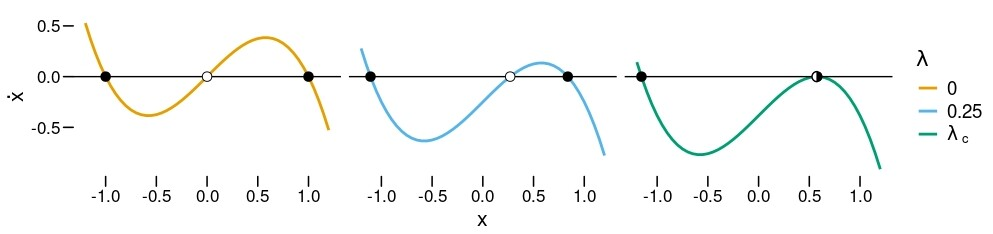
\includegraphics[scale = .14]{figures/double_well_plot.jpeg}
        \caption{The flow of the DW-potential dynamical system for varying values of $\lambda$.}
        \label{figure:DW_dynamic_plot}
    \end{center}
\end{figure}\\
By definition, the fixed points are the zeroes, which is typically marked as points in graphical representations. As a convention, stable fixed points are solid points, whereas unstable are hollow. Whether a specific fixed point is stable or unstable is easily deduced by simply looking at the flow of the graphs. When $\dot{x}_t$, i.e. $x_t'$, is below 0, the flow is to the left and vice versa; this simple reasoning allows us to understand the systems without doing any computations.

Now, notice the curious things happening for the value $\lambda = \lambda_c$. The system goes from having three fixed points: Two stable and one unstable, to just two fixed points: One stable and one half-stable. Mathematically, there is a real double root at the half-stable fixed point. Looking at the graph it is clear that this change in $\lambda$ results in a rather different qualitative behaviour of the system. From the definition of the double-well potential it is not difficult to see that increasing the value further would leave the system with just one stable fixed point. This is an entirely different overall behaviour compared to the other values of $\lambda$. This type of change in the characteristics of a dynamical system, we call a bifurcation. The specific value, $\lambda_c$, for which the changes occurs, we refer to as bifurcation points.\cite{Strogatz2019_gv} In applications, these points are also sometimes refered to as tipping points and the phenomenon as tipping.
To get an understanding of why this is occuring in this specific system, we compute the cubic discriminant. For a cubic polynomial in depressed form such as the dynamic (\ref{eq:originalDW}), this quantity is
\begin{align}
    \Delta_{\mathrm{DW}} = -\left(4(-1)^3+27\left(\lambda\right)^2\right) = -27\lambda^2 + 4. \label{eq:DW_discriminant}
\end{align} 
Whenever the result is positive; there are three solutions, when it is zero, there are two solutions. Finally, for negative values, there is only one solution to the cubic polynomial. The discriminant is a second degree polynomial in the parameter $\lambda$ and it has roots $\pm \frac{2}{3\sqrt{3}}$. The system depicted in figure \ref{figure:DW_dynamic_plot} uses the positive root as the value of $\lambda_c$. Yet, it is not difficult to imagine that decreasing the value of $\lambda$ would result in a mirrored, but completely analagous qualitative change to the one we observe in figure \ref{figure:DW_dynamic_plot}. Mathematically, this is due to $\Delta_{\mathrm{DW}}$ being positive for values of $\lambda$ between the two roots and negative outside. In the following, we focus on the positive root; though it should be noted that our reasoning is not limited to this bifurcation point. \\\\
$\lambda_c$ and the half-stable fixed point pertaining to it constitute an example of a specific type of bifurcations known as saddle-node bifurcations. For this value of $\lambda_c$ the stable fixed point is found at $x_1^* = -\frac{2}{\sqrt{3}}$, and the half-stable is $x_2^* = \frac{1}{\sqrt{3}}$. These are the solid- and partially solid points on the right graph in figure \ref{figure:DW_dynamic_plot}. We study the behaviour of the system close to the pair $(x, \lambda) = (x_2^*, \lambda_c)$ by a Taylor expansion of $f_{\mathrm{DW}}$ to the second order around the $x$-value and first order around the $\lambda$-value. This yields
\begin{align}
    f_{\mathrm{DW}}(x_t,\lambda)&\approx \frac{\partial}{\partial x_t}f_{\mathrm{DW}}(x_2^*,\lambda_c)(x-x_2^*) + \frac{1}{2}\frac{\partial^2}{\partial x_t^2}f_{\mathrm{DW}}(x_2^*,\lambda_c)(x_t-x_2^*)^2 \nonumber \\
     &+ \frac{\partial}{\partial \lambda}f_{\mathrm{DW}}(x_2^*,\lambda_c)(\lambda - \lambda_c) = -\sqrt{3}\left(x_t-x_2^*\right)^2 - \left(\lambda - \lambda_c\right) \nonumber \\&= -\left(\tilde{x}_t^2 + \tilde{\lambda}\right), \label{eq:prototypicalSaddleNode}
\end{align}
where $\tilde{x}_t = 3^{\frac{1}{4}}\left(x_t-x_2^*\right)$ and  $\tilde{\lambda} = \lambda - \lambda_c$. That is for values close to the bifurcation point the dynamic behaves similarly to that of this function, which is a quadratic polynomial in $x$ and linear in $\lambda$. Not only, is it a quadratic is $x$, it is also a rather simple quadratic with linear and intercept terms equal to zero. With $x_2^*$ being a fixed point, this was expected for the intercept. However, that the derivative of $f_{\mathrm{DW}}$ also evaluated to zero was not obvious. In fact, systems with bifurcations that locally around its bifurcation point behave in this manner are exactly what we understand by a system with saddle-node bifurcation. It is clear that any system with this type of Taylor-expansion around the bifucartion point will have a saddle-node bifurcation, as we can always scale and shift the dynamics to that of (\ref{eq:prototypicalSaddleNode}). For this reason, this particular form of dynamics is known as the prototypical- or normal form of the saddle-node bifurcation. Similar, calculations for the other bifurcation point of the double well model will leave us at the additive inverse of \ref{eq:prototypicalSaddleNode}. So in complete generality the normal form is
\begin{align}
    \mathrm{d}x_t = \pm\left(x_t^2 + \lambda\right)\mathrm{d}t
\end{align} 
As we see in the calculations of (\ref{eq:prototypicalSaddleNode}), these forms do not care about scaling and shifting, whence we write the normal form as
\begin{align}
    \mathrm{d}x_t = \pm\left(A\left(x_t - m\right)^2 + \lambda\right)\mathrm{d}t, \label{eq:standardform}
\end{align}
where $A>0$. Note that $x_t$ is not the same as the one from the double-well potential from earlier; we live with this ambiguity to avoid introducing too much notation.\\ In sum, we have illustrated that for some systems, which change qualitative behaviour at some parameter values; these systems behave roughly as what we refered to as the normal form of the saddle-node bifurcation, when $\lambda$ is close to the bifurcation point. Studying the system (\ref{eq:standardform}), we first note that is has quadratic discriminant $\Delta_{\mathrm{sf}} = -4A^2\lambda$. That is, we have two solutions to \ref{eq:standardform}, i.e. the system has two fixed points, whenever $\lambda<0$, one fixed point for $\lambda = 0$ and zero otherwise. When they exist, the fixed points are given by
\begin{align}
    \mu\left(\lambda\right) = m \pm \sqrt{-\frac{\lambda}{A}}. \label{eq:fixedPoint}
\end{align}
The fixed points are one stable- and one unstable fixed point, when $\lambda<0$; and one half-stable when $\lambda=0$. Which of the two is stable or unstable depends on the sign of the normal form \ref{eq:standardform}. Instead of illustrating the bifurcation qua the flow graph, we depict the phenomenon with a so-called bifurcation diagram\\
\begin{figure}[h]
\begin{center}
    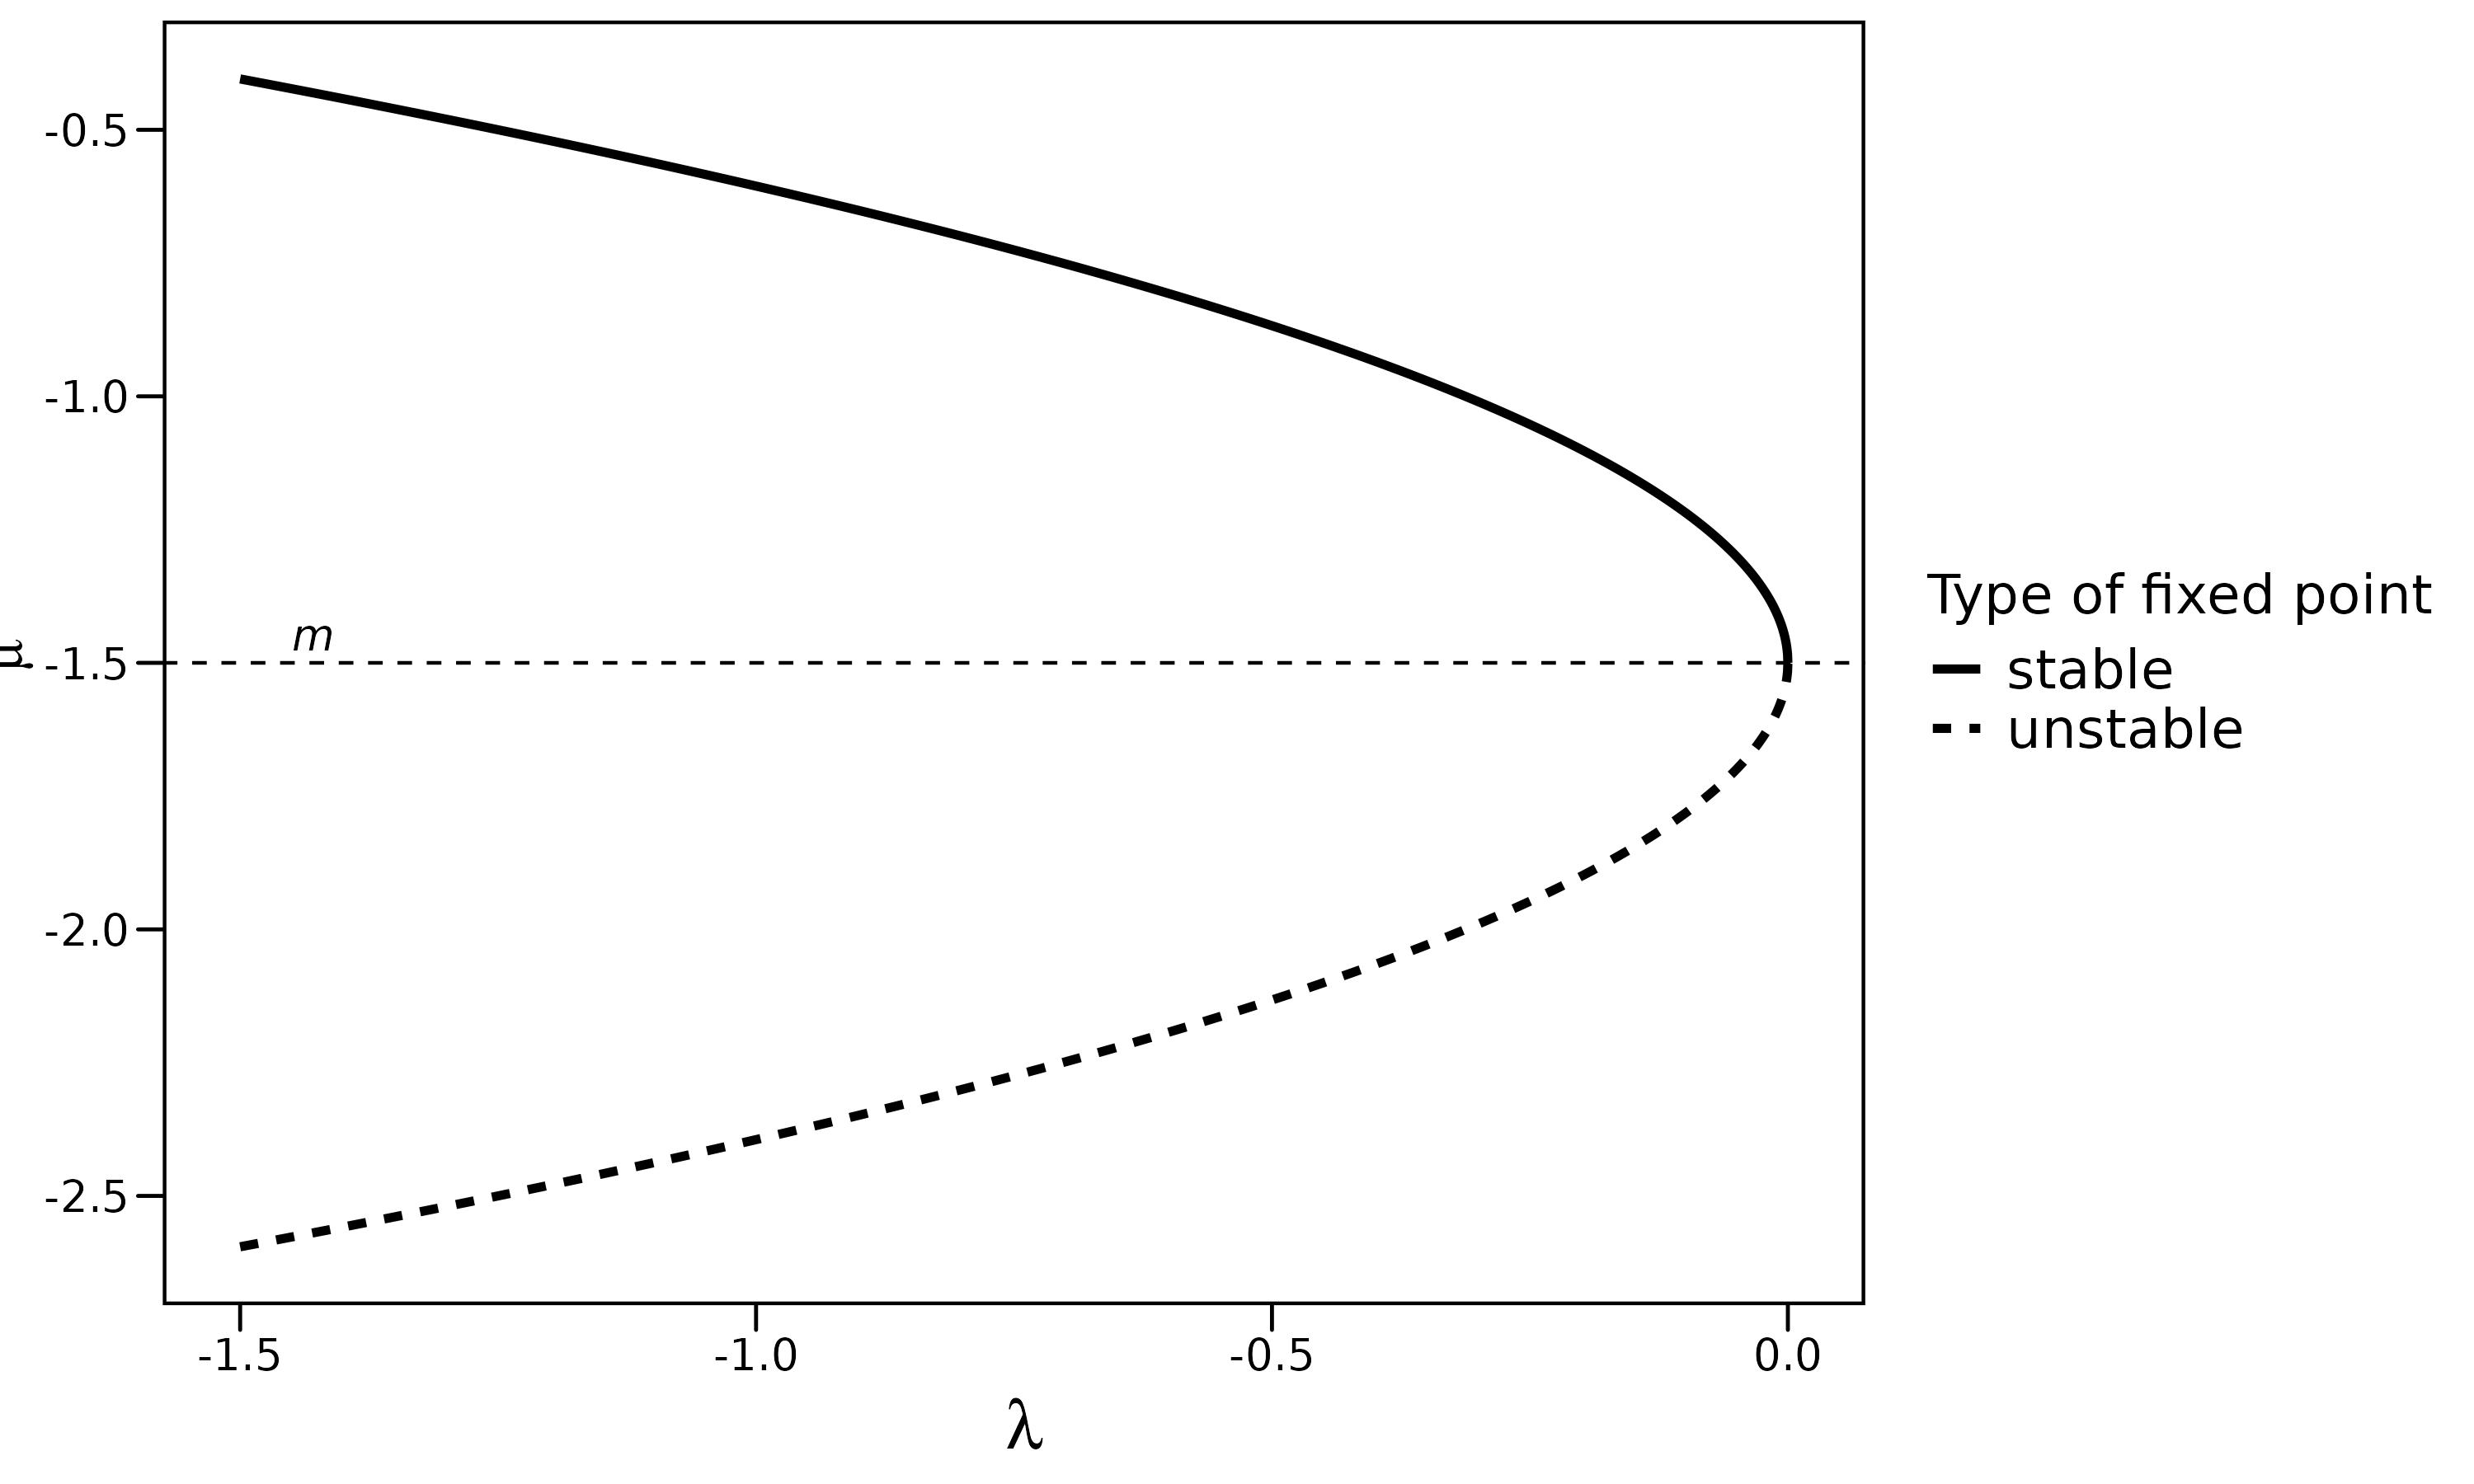
\includegraphics[scale = .125]{figures/bifurcation_diagram.jpeg}
    \caption{Bifurcation diagram of the scale and shifted normal saddle-node bifurcation.}
    \label{figure:bifurcationDiagram}
\end{center}
\end{figure}\\
Note that for $A$ and $m$ we picked $0.8$ and $-1.5$ respectively. The bifurcation diagram in figure \ref{figure:bifurcationDiagram} are the epitome of such diagrams for systems with a saddle-node bifurcation. As we have illustrated, any system with this type of bifurcation will locally for $\lambda \approx \lambda_c$ resemble (\ref{eq:standardform}) and hence their bifurcation diagram will too. One can also do the computations for the other branch of the normal form. In this case the fixed points in the bifurcation diagram are the same as before barring the fact that the types of the fixed points are swapped, i.e. for this system figure \ref{figure:bifurcationDiagram} would be mirrored around $m$.
\subsubsection{Tipping points}
We are now equipped with the necessary vocabulary to understand the model with which we estimate tipping points. We do not assume anything particular about the overall system dynamic other than that the system has a saddle-node bifurcation. Thus, we know that sufficiently close to the bifurcation point, we can consider the scaled and shifted prototypical saddle-node bifurcation system (\ref{eq:standardform}) in the general system's stead. For fixed $\lambda < 0$ in (\ref{eq:standardform}) the system is overall stable and converges to the stable fixed point, when we are not too far away from it. However, there are values, where the flow  diverges. Imagine that we are in the negative branch of (\ref{eq:standardform}); this is the situation depicted in figure \ref{figure:bifurcationDiagram}. As can be seen in the graph, the system diverges even when $\lambda<0$, if the process finds itself below the unstable fixed point. Furthermore, when $\lambda>0$ the system always diverges.

To estimate a tipping point with this model, is to estimate a point in time or the occurence of an event at which this abrupt change in characteristic of the system happens. Typically, this is done as a time point, which is also what we will do by modelling a ramping of $\lambda$ from some base value $\lambda_0$ it finds itself in, when the system is stable overall. We imagine that when we have observed the system for some time, $t_0$, it is disturbed or altered in some way that begins the ramping. There are several different ways this can be modelled, but here we let $\lambda$ depend on time, $t$, explicitly in the following way
\begin{align}
    \lambda_t = \lambda_0\left(1 - \max\left\{\frac{t - t_0}{\tau_c},0\right\}\right)^\nu, \label{eq:lambdaRampDefinition}
\end{align} 
which is the model from \cite[equation (2)]{Ditlevsen2023} with the addition of the parameter, $\nu>0$. As said $t_0$ can be understood as the time when ramping of $\lambda_t$ starts. The parameter $\tau_c$ is the amount of time after ramping begins for $\lambda_t$ to become zero. This is the point, when the two fixed points in \ref{figure:bifurcationDiagram} become one. That is, the point in time, where the dynamics of the system changes significantly: The tipping point. \\\\
Now, it is crucial to understand that the normal form is only a good approximation for a system with a saddle-node bifurcation close to its bifurcation point. Far from the tipping point or after the system has tipped the dynamics of the normal form are no longer a good approximation of the underlying dynamics. Put differently, our model does not allow us to infer anything about the system after it has tipped. Furthermore, we must observe the system sufficiently close to the bifurcation point for the dynamics to be close to the normal form. How close depends on the system at hand. These facts are, of course, significant downsides to the model. However, having such lean assumptions results in simple models: We can be completely agnostic about the actual dynamics of the system, because our main interest is the behaviour close to- or at the bifurcation point. As long as they have a saddle-node bifurcation, these dynamics could be arbitrarily complex and possibly difficult to infer anything about. Potentially, (\ref{eq:standardform}) is a huge simplification.
\subsubsection{Tipping in stochastic systems}
As is done in \cite[equation (1)]{Ditlevsen2023}, we introduce stochasticity into the normal form (\ref{eq:standardform}) to model the various uncertainties in the system. To reiterate from our introducing of stochastic differential equations, this results in a shift in the understanding of the solution, $X_t$. Now, for each point in time, $t$, the solution, $X_t$, to the noisy standard form has some distribution. While the original work assumed additive noise; we model the stochastic term as having the same noise as one of the Pearson diffusions (\ref{eq:pearsonDiffusion}). In sum, the model we consider is
\begin{align}
    \mathrm{d}X_t = \pm\left(A\left(X_t - m\right) + \lambda_t\right)\mathrm{d}t + \sigma\sqrt{\left(aX_t^2 + bX_t + c\right)}\mathrm{d}W_t, \label{eq:standardStochasticForm}
\end{align}
with $\lambda_t$ given by (\ref{eq:lambdaRampDefinition}). Note that the constants: $a, b$ and $c$ are picked such that the square-root is well-defined. In particular, we use the stochastic terms from the ergodic Pearson diffusions from table \ref{table:ergodicDiffusions}. To refer to a specific model, we have coined the following nomenclature: We refer to a model via the Pearson diffusion from which it gets its stochastic term. This could for instance be the \textit{$t$-diffusion based} model or even the \textit{$t$-distribution} model, albeit the last name might be a bit confusing or misleading it is quite natural to use. Alternatively, we might refer to the models by the way the noise enters, such as the model with \textit{linear} noise or the model with \textit{additive} noise. Although it might be obvious, it needs to be pointed out that a specific model inherits the state space of the pearson diffusion it shares stochastic term with in the way that the state space of models are always subspaces of the state space of the Pearson diffusion. The state spaces can be seen in table \ref{table:ergodicDiffusions}. Though, in this case the specific drift term in (\ref{eq:standardStochasticForm}) implies that the state space of a model correspond exactly to the state space of the Pearson diffusion it uses.\\\\
For clarity, $W_t$ is a brownian motion defined in (\ref{eq:brownianMotion1})-(\ref{eq:brownianMotion3}). This means that the solution to (\ref{eq:standardStochasticForm}) is an Ito process. Extending dynamical systems in this way is commonplace in various applied settings such as physics or finance. As said earlier, a way we typically motivate these kinds of constructions is, if we have a deterministic model for the well understood dynamics of the system. This could for instance be the drift term of (\ref{eq:standardStochasticForm}), which models the general behaviour of the system well: in this case that it has a saddle-node bifucartion. However, in the real world there might be elements that cannot be captured by the drift. Introducing a stochastic term into the dynamics lets us model the fact that there are parts of the system we do not understand or we do not want to model deterministically, because they are too complicated. Alternatively, we could use stochastic modelling, because our measurements are too inaccurate or noisy in some manner \newpage
\noindent With the scalar weak order 2.0 Ito-Taylor method described in section (\ref{subsubsec:Discretization}) we draw three sample paths with the same realizations of $W_t$ for each of the models to illustrate how they differ. In the graph one row corresponds to one path. The model we use is the one with a negative sign in front of the drift in (\ref{eq:standardStochasticForm})
\begin{figure}[h]
    \begin{center}
        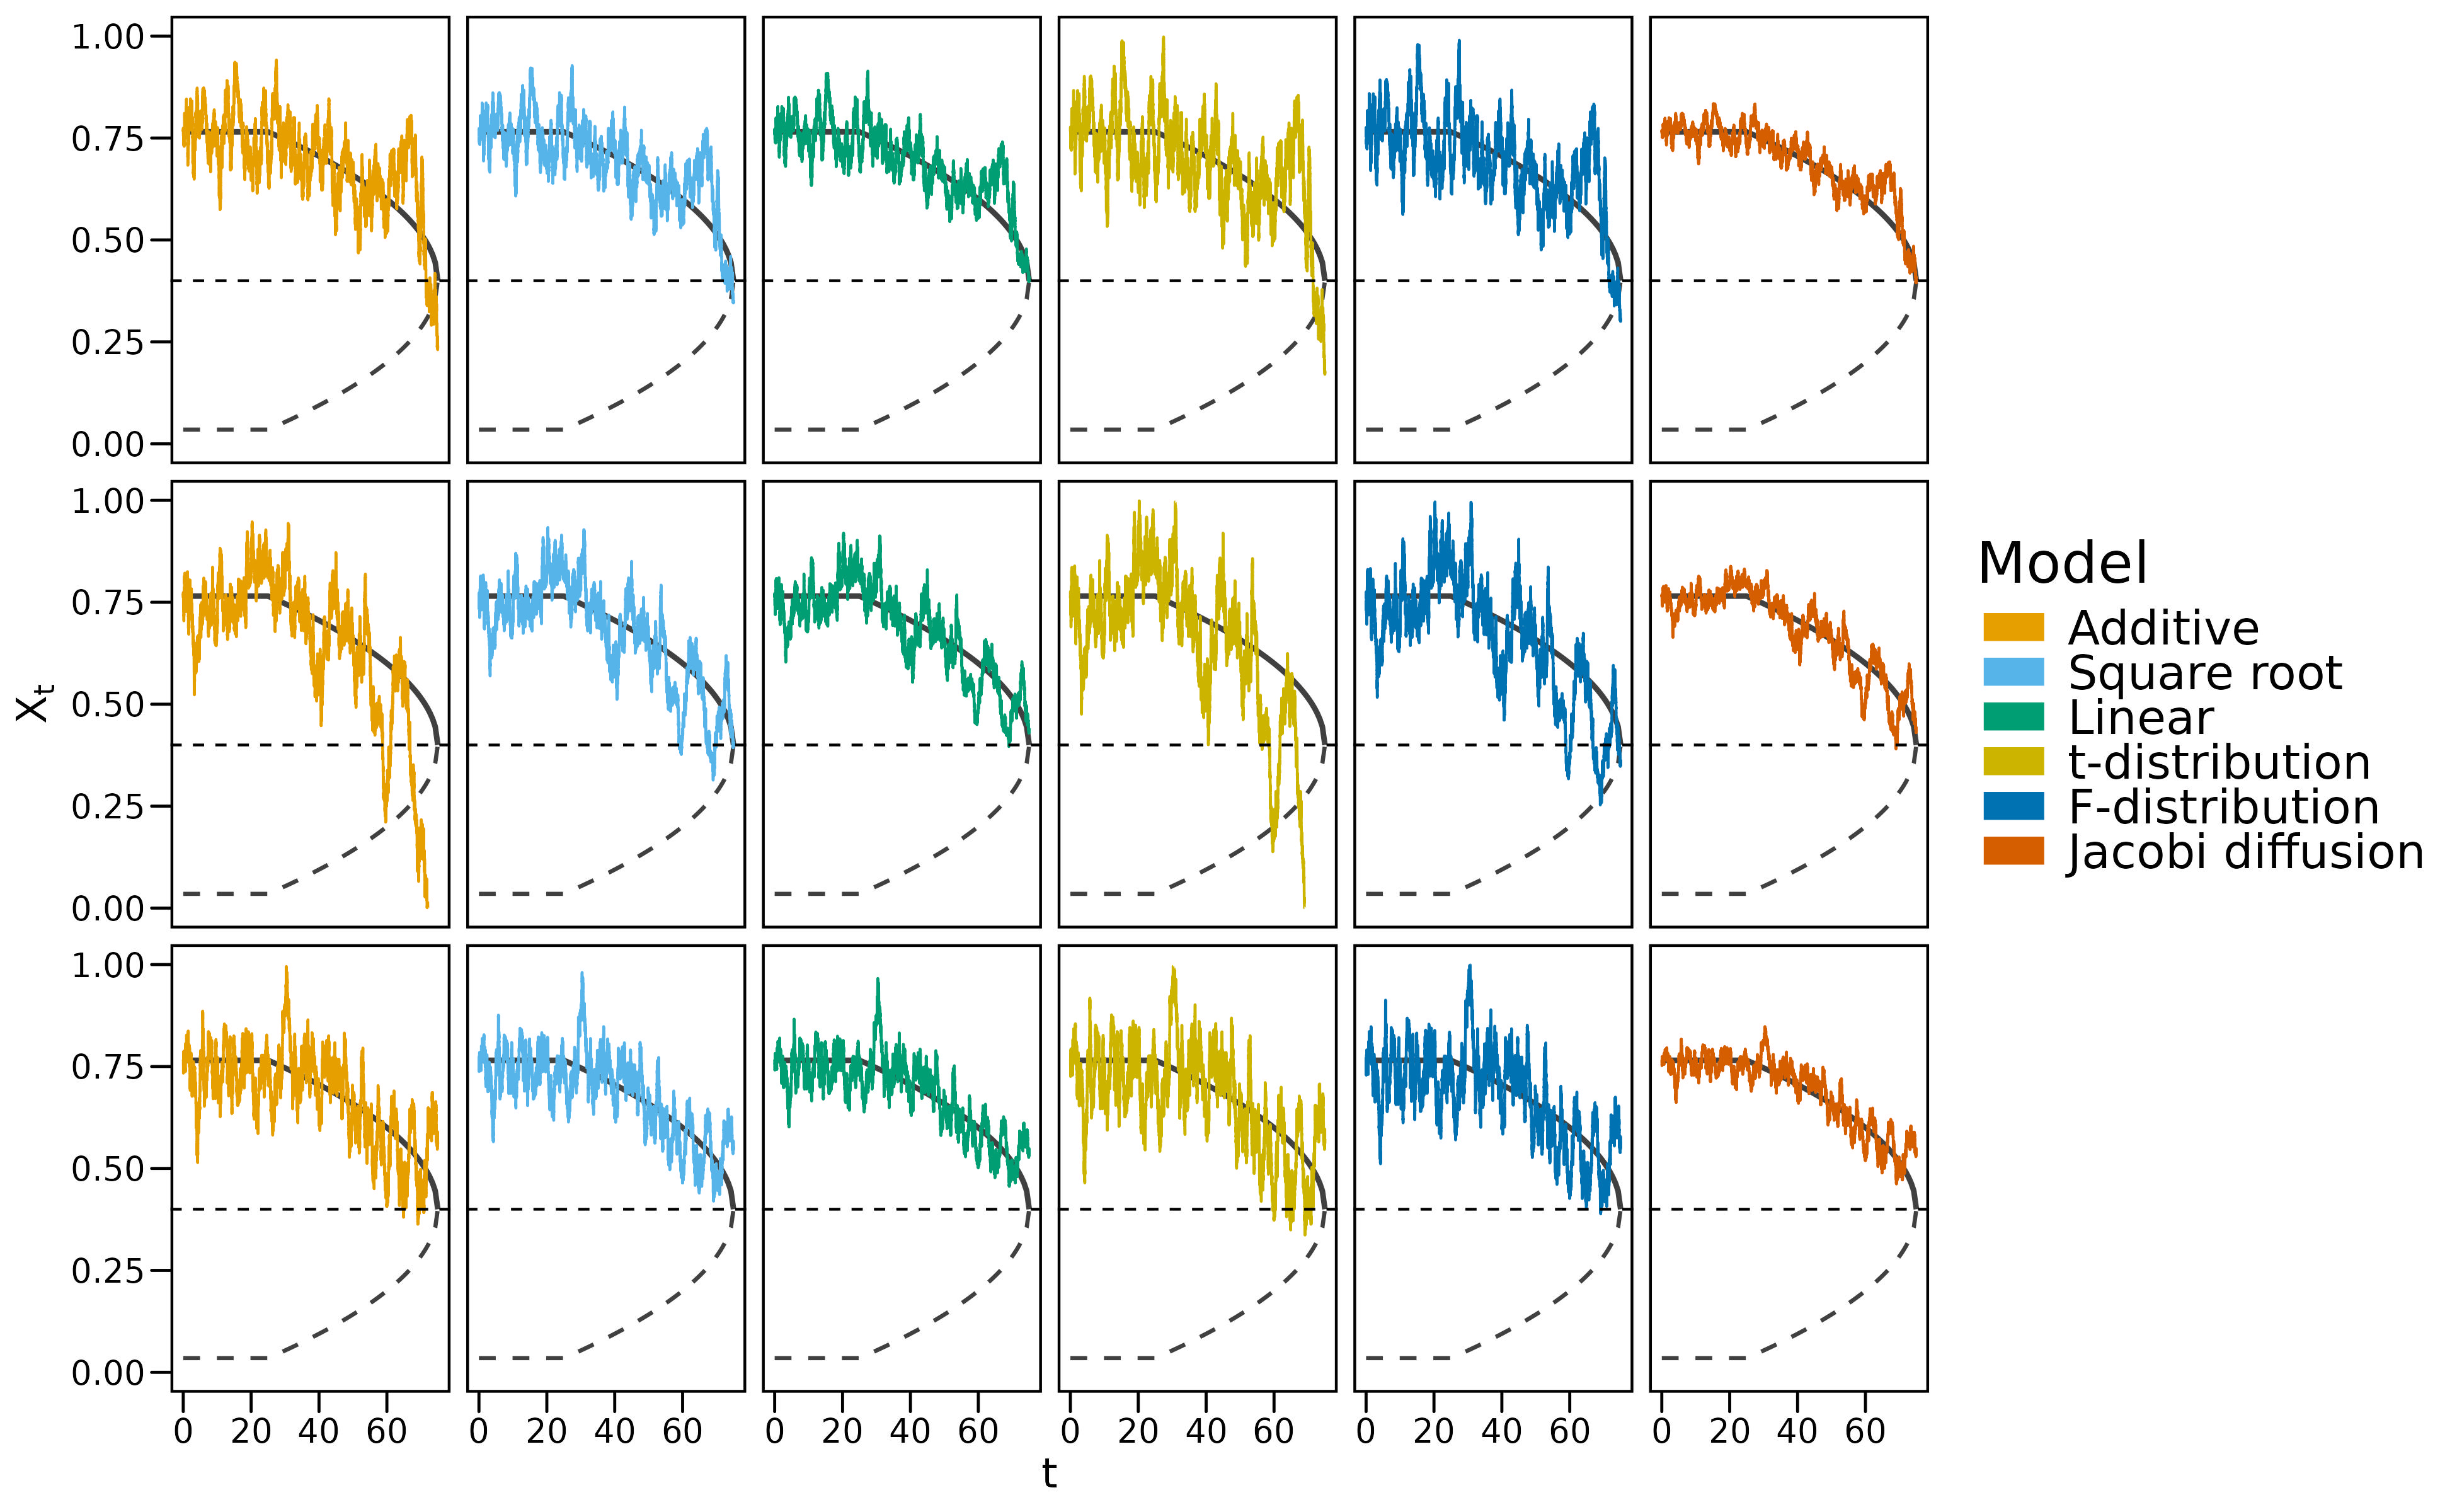
\includegraphics[scale = .1]{figures/sample_paths_plot_small_scale.jpeg}
        \caption{The dynamics of (\ref{eq:standardform}) with the six different noise terms from table (\ref{table:ergodicDiffusions}) applied to the same three realizations of a brownian motion.}
        \label{figure:samplesFromAllDifferentModels}
    \end{center}
\end{figure}\\
All the samples were drawn with parameters, $A = 1.5, m = 0.4, \lambda_0 = -0.2, \sigma = 0.1$ and $\nu = 1$. These parameters are carefully selected to ensure that we are in the state space of all processes in table \ref{table:ergodicDiffusions}. The process is started at time $0$ in its stable fixed point and starts ramping at $t_0 = 25$. The bifurcation point was set at time $75$, which means that $\tau_c = 50$. In sum, this means that in accordance with (\ref{eq:fixedPoint}) and (\ref{eq:lambdaRampDefinition}) the stable and unstable fixed points start moving from $m\pm\sqrt{\frac{\lambda_0}{A}}$ at time $t_0$ toward $m$ at time $t_0 + \tau_c$. Similarly to figure (\ref{figure:bifurcationDiagram}) this is depicted using a solid and dashed line respectively. The smaller horizontal dashed line they meet at is naturally, $m$. This is the effect of the specific form of ramping in (\ref{eq:lambdaRampDefinition}) when $\nu = 1$, i.e. a square-root evolution of the fixed points towards $m$ at the tipping point. This is exactly the effect of the ramping model from \cite{Ditlevsen2023}. Regardless of the noise, all the models have a bifurcation tipping at time $t_0+\tau_c$, the point we have simulated up to. However, due to the random nature of the brownian motion in the stochastic term not all models tip at that point. As we discussed with regards to figure \ref{figure:bifurcationDiagram}, the deterministic part of the process will diverge from below the unstable fixed point. We see that the additive noise model as well as the model with stochastic term from the ergodic diffusion with the $t$-distribution as its stationary distribution, cross the unstable fixed point prematurely twice. This phenomenon is called noise induced tipping and is exclusively a phenomenon in the study of dynamic system with stochasticity. All of the models are, in principle, always able to tip via noise. Still, for this to have any significant chance of happening the noise has to be on a scale that compares with the jump the process needs to make. In our case, this jump is the distance between the stable- and unstable fixed points at any given time point. However, the closer the path gets to the bifurcation point, the smaller the jump has to be. This is also why, we actually see the square-root- and linear noise based models as well as the $F$-diffusion model tip a bit before the bifurcation point in the first scenario. It should also be mentioned that a dynamic with a stochastic term does not have to have saddle-node bifurcation for it to be able to experience noise induced tipping.\\\\
Now, from table \ref{table:ergodicDiffusions} it is clear that the model with the same noise as the diffusion with the $t$-distribtion as its stationary distribution will always have diffusion term at least as large as the additive noise model. Thus, for the same realizations of $W_t$, if the model with additive experiences noise-induced tipping, it is quite likely that the $t$-diffusion based model will so too. The difference in the stochastic terms will be even more pronounced the further the values are from zero. This is also true for some of the other models. In figure \ref{figure:samplesFromAllDifferentModels} we have chosen parameters such that we are on the unit interval. This is to accomodate for the relatively confined state space of the Jacobi-diffusion based model. If we disregard this model, all the processes are well-defined on at least the positive reals. To illustrate what role the scale of our observations plays on the noise. We use first two Wiener realizations from earlier and depict the paths with the same $t_0, \tau_c, \sigma, A$, but to shift the scale away from the unit interval, we have picked $m = 3$ and $\lambda_0 = -1.75$. We get the following results
\begin{figure}[h]
    \begin{center}
        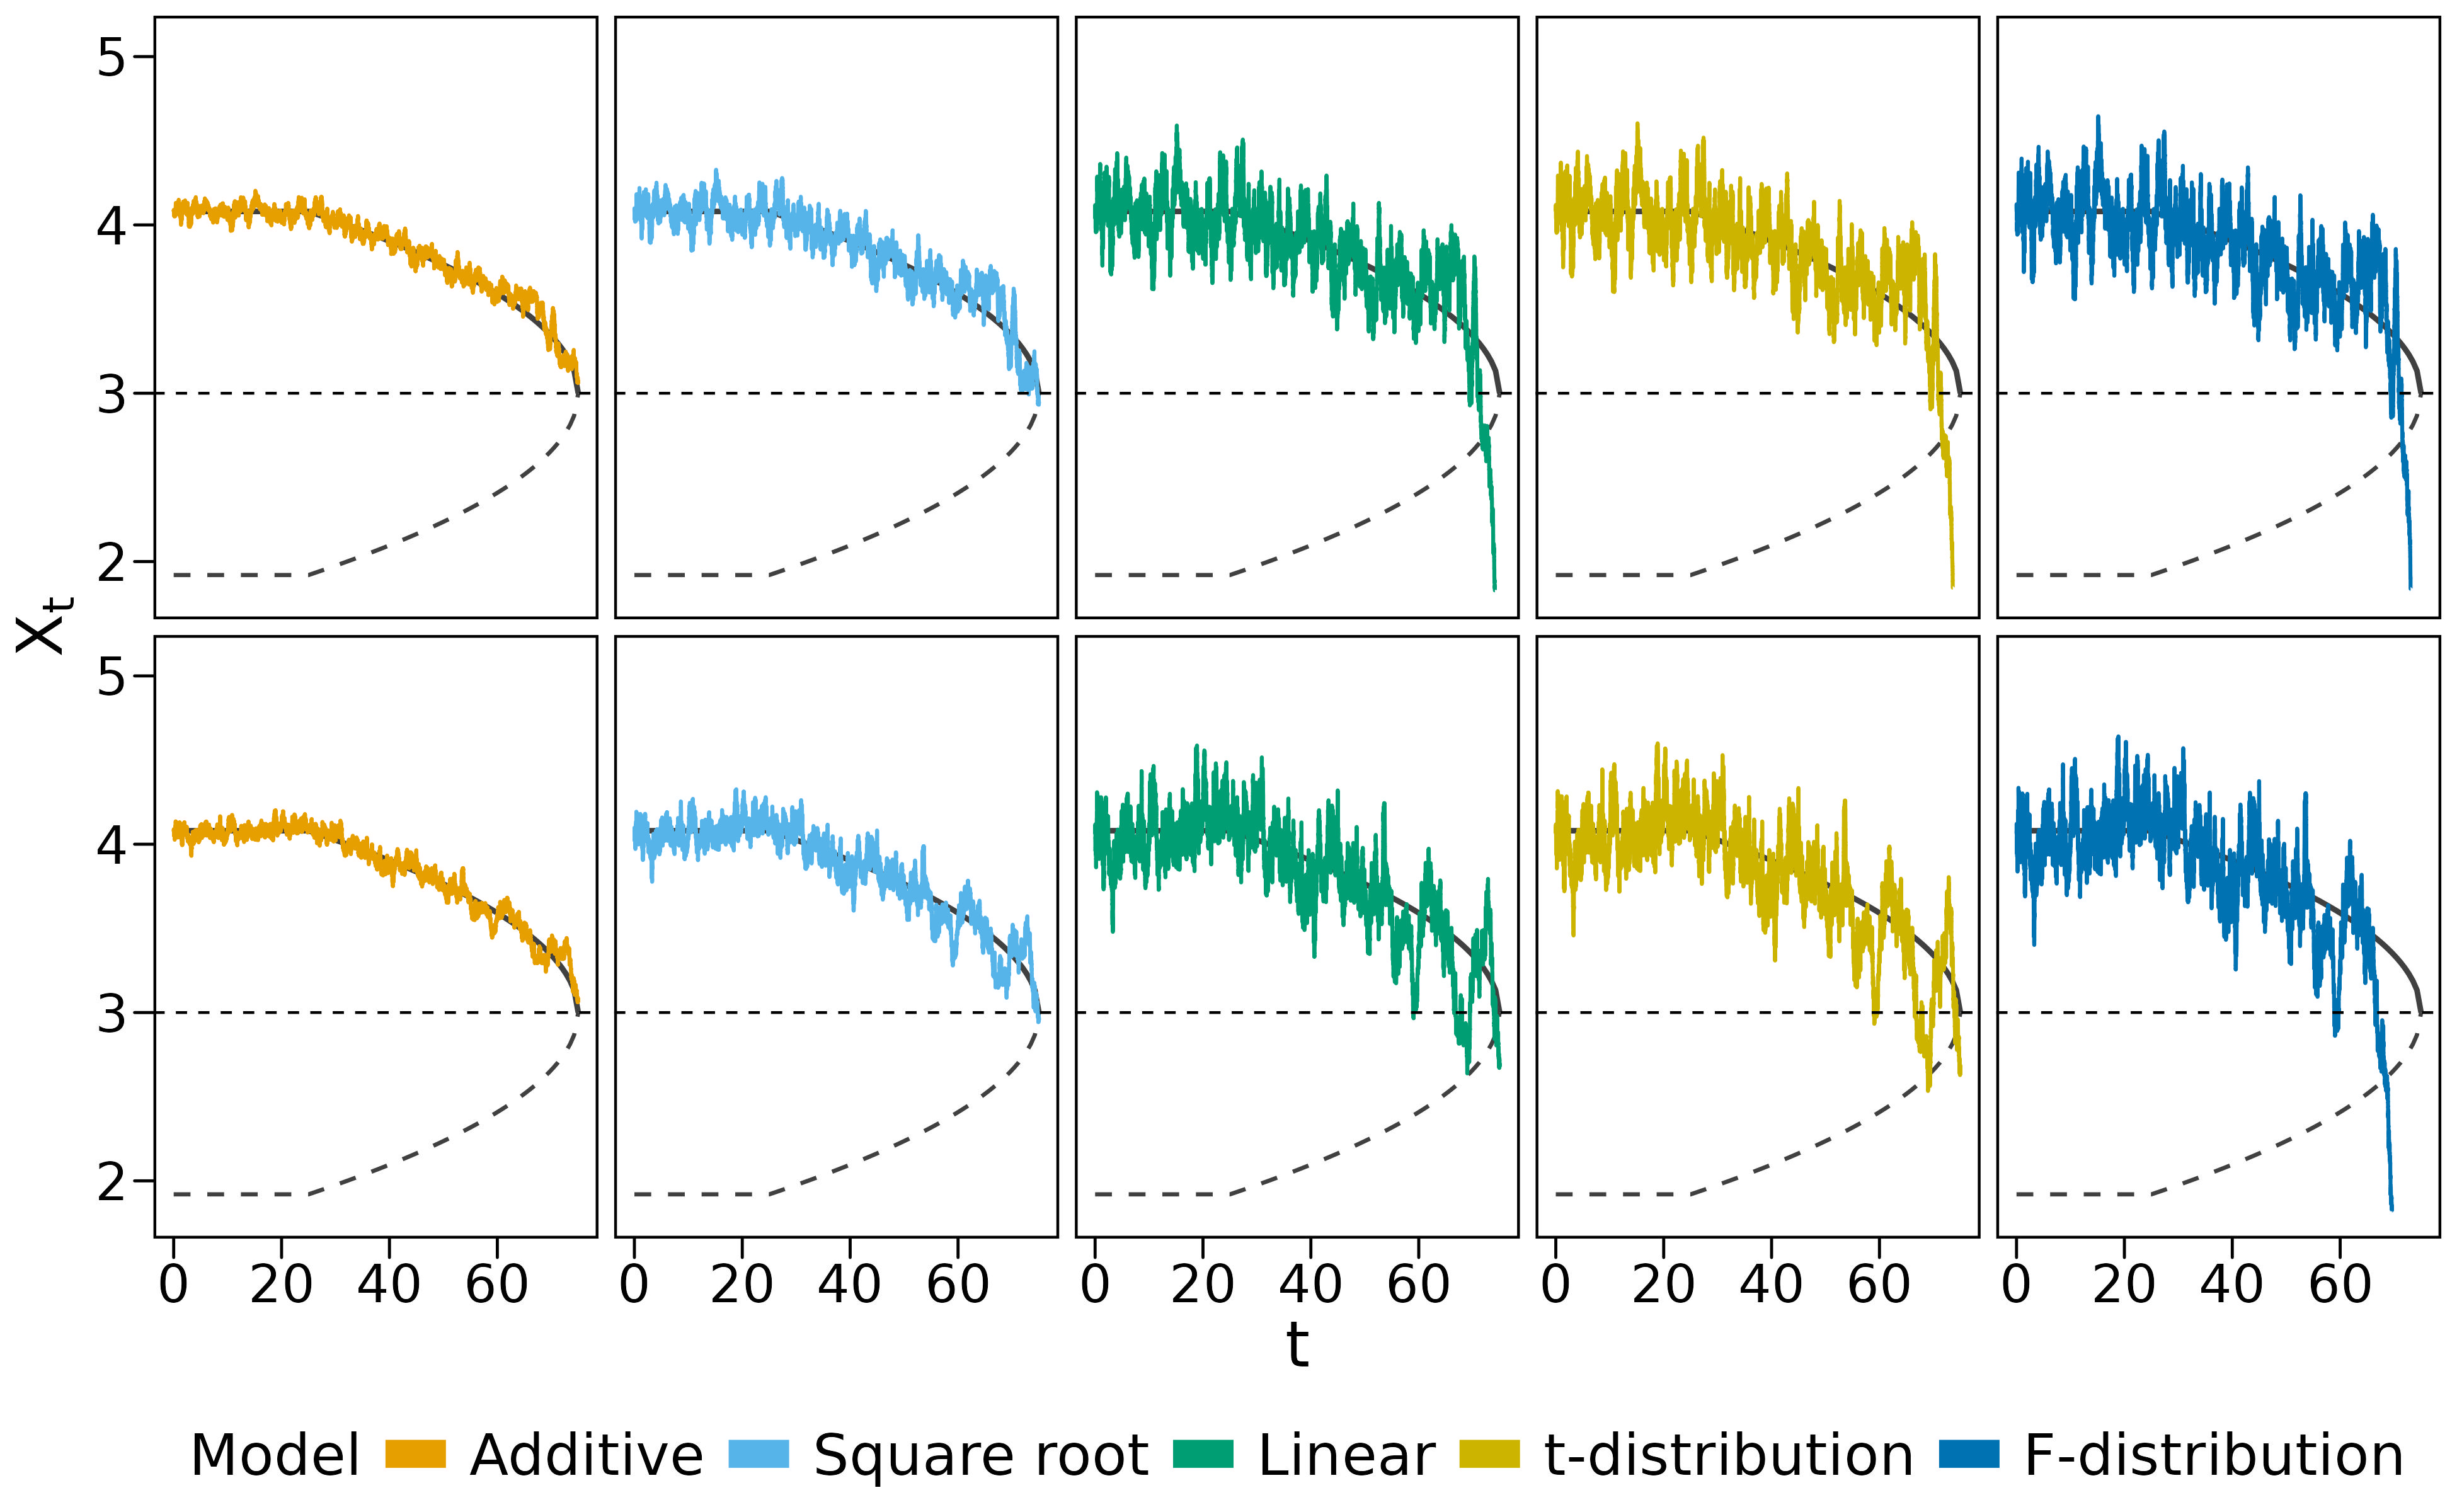
\includegraphics[scale = .1]{figures/sample_paths_plot_big_scale.jpeg}
        \caption{The dynamics of (\ref{eq:standardform}) shown on a different scale than figure \ref{figure:samplesFromAllDifferentModels} but with the same realizations of the Wiener process.}
        \label{figure:samplesFromFiveDifferentModels}
    \end{center}
\end{figure}\\
The overall impression of the respective models is quite different in figure \ref{figure:samplesFromFiveDifferentModels} than figure \ref{figure:samplesFromAllDifferentModels}. There is very little noise in the additive model in comparison to the other models with some kind of multiplicative noise. For instance the effect of the diffusion term in the $t$-diffusion based model is quite evident here. In addition, we observe how the $F$-diffusion based model along with the linear and square-root models undergo noise-induced tipping. Looking at the noise of the paths, it is clear what the difference in scale has meant for the qualitative feel of the square-root- and linear models. In figure \ref{figure:samplesFromAllDifferentModels} the square-root model was more noisy, while the opposite is the case in figure \ref{figure:samplesFromFiveDifferentModels}; here the linear model is more noisy. All this is not too surprising, when looking at the diffusion coefficients for the two processes. Neither is it surprising that the $F$-diffusion based model appear more noisy than both of them in both scales.\\\\
Lastly, we remark on the effect of the $\nu$-parameter, which is an extension of $\lambda_t$ \cite[equation (2)]{Ditlevsen2023}. As said this model corresponds to $\nu = 1$ as $\nu$ enters in an exponential manner into the bifucartion-parameter, which governs the fixed point of the drift according to \ref{eq:fixedPoint}. Apart from this fact the model works the same: $\lambda_t = \lambda_0$ for $t<t_0$, where ramping begins and $t=\tau_c + t_0$ is the tipping point. We use the same values of $m$ and $A$ as in figure \ref{figure:bifurcationDiagram} and pick $\lambda_0 = -2$, $\tau_c = 100$ and $t_0 = 10$, for the illustration of the fixed points as a function of time and $\nu$ in the model (\ref{eq:lambdaRampDefinition})
\begin{figure}[h!]
    \begin{center}
        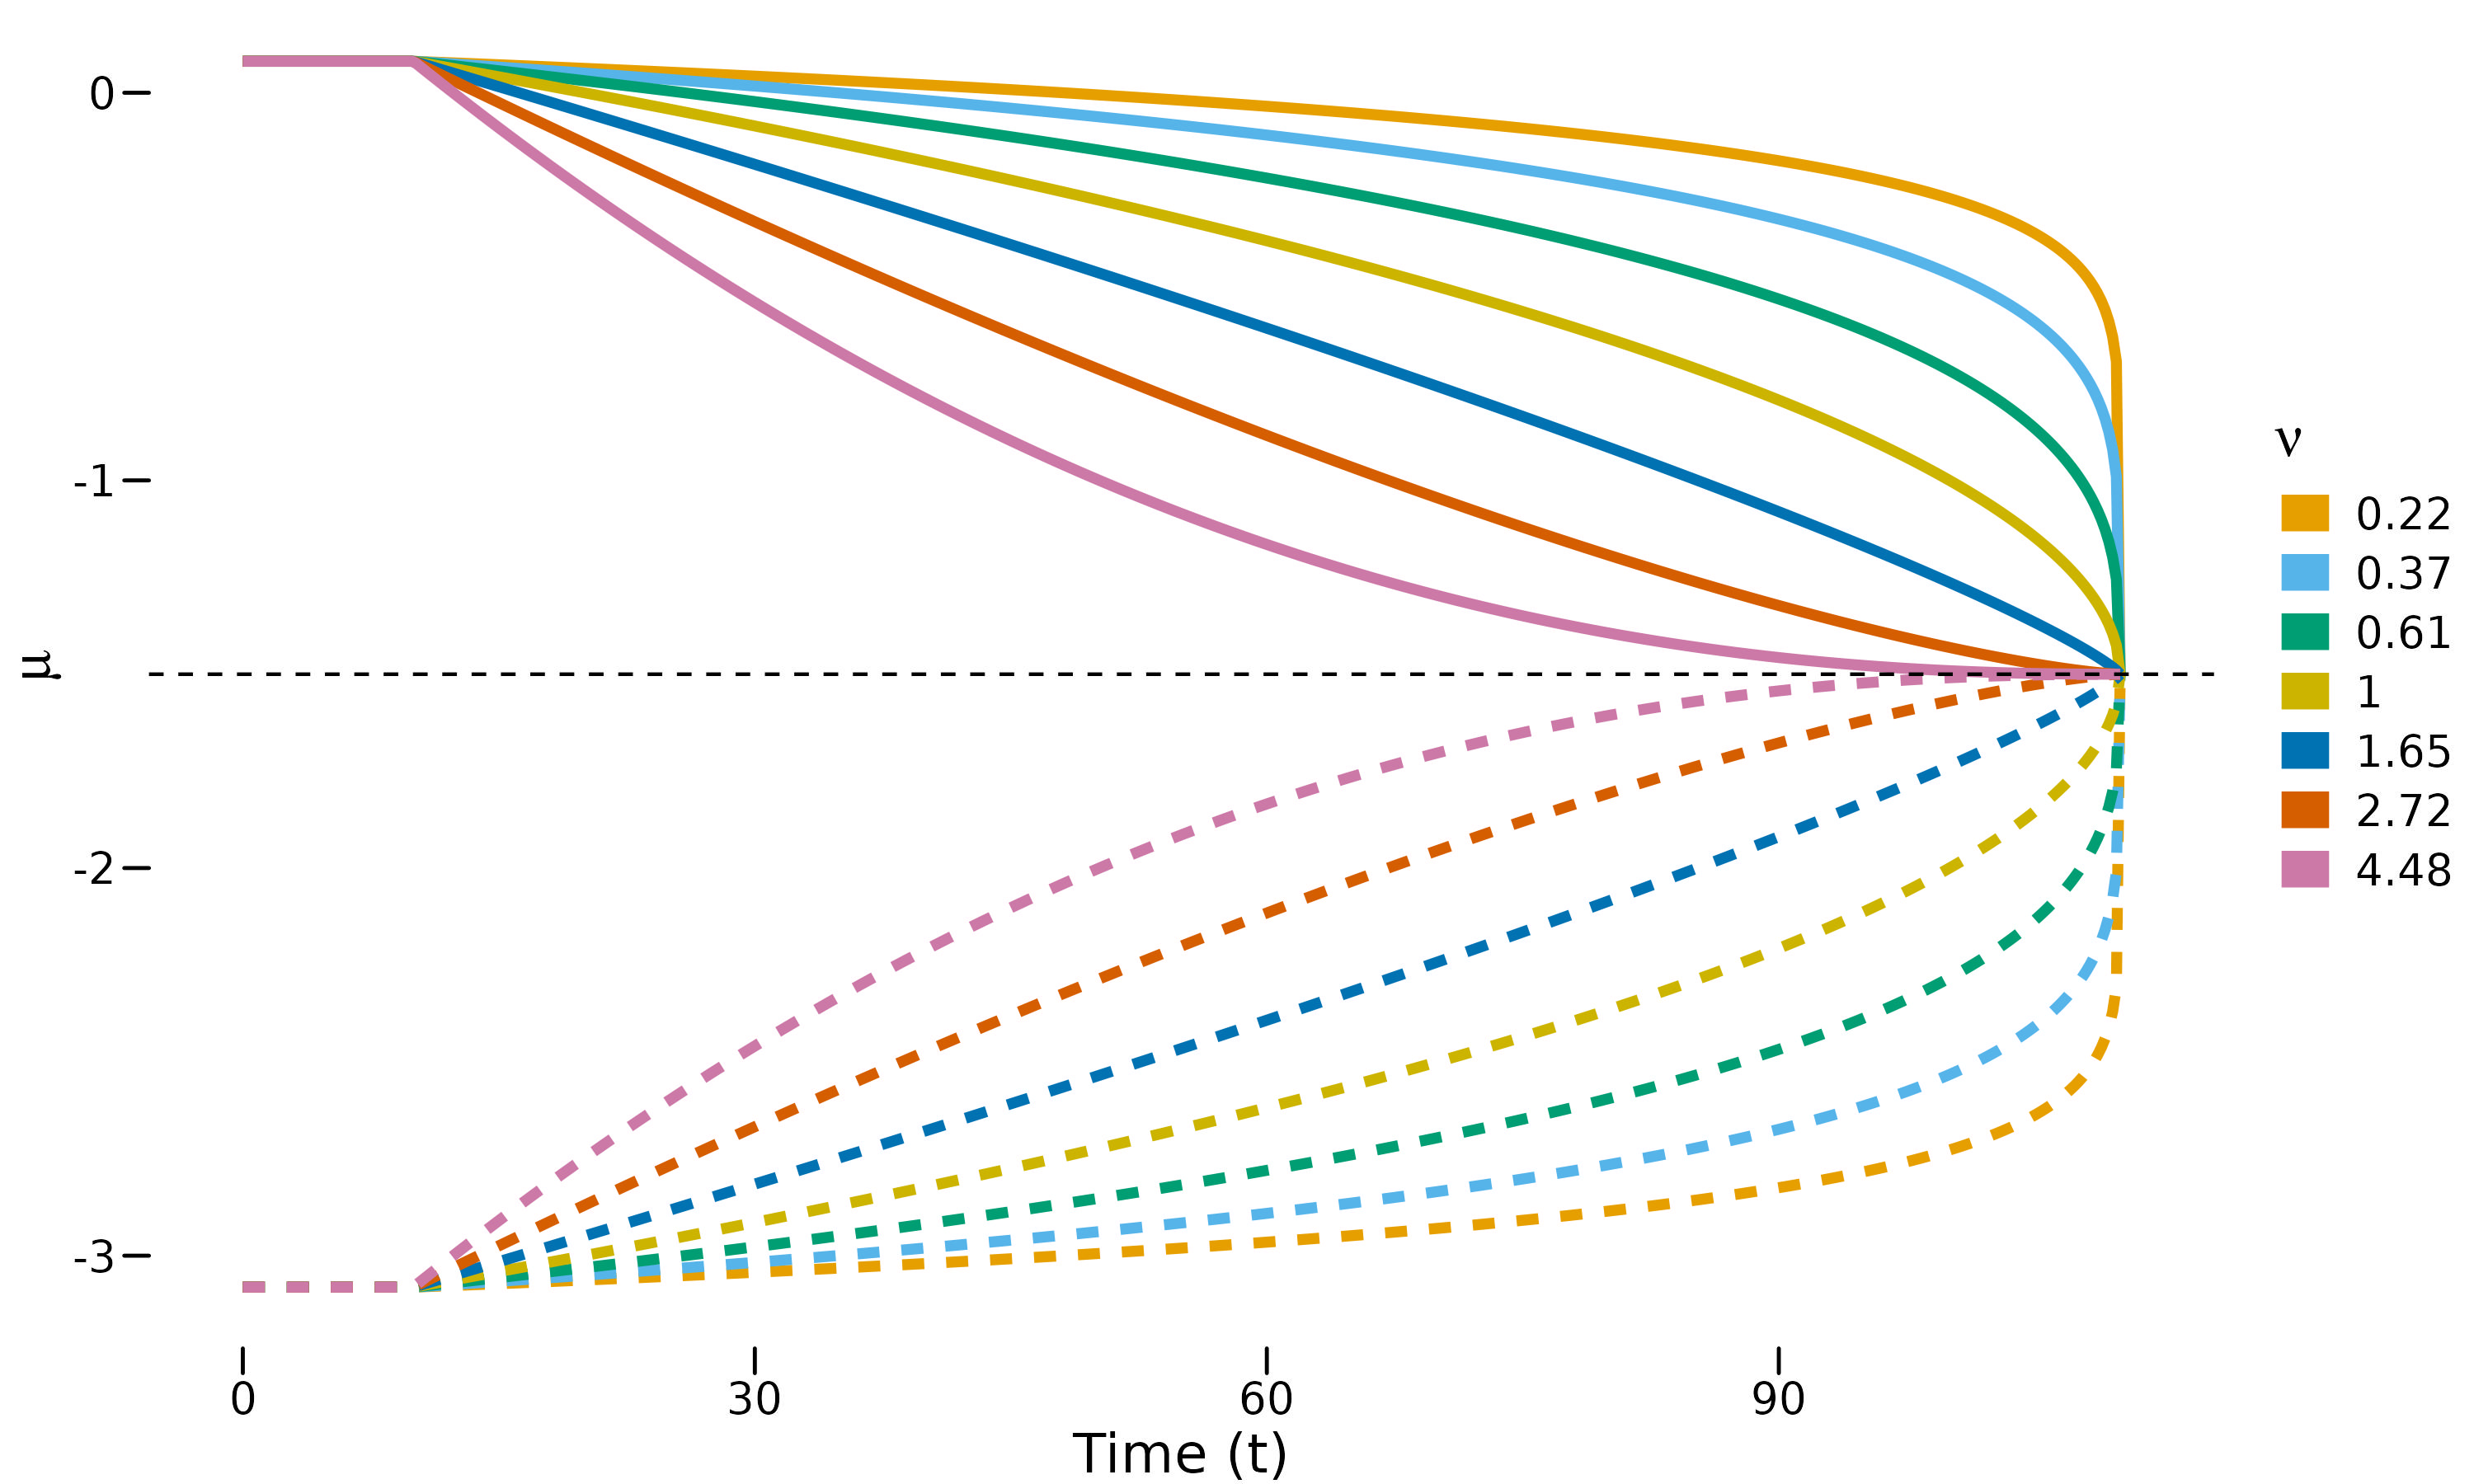
\includegraphics[scale = .1]{figures/nu_plot.jpeg}
        \caption{The fixed points of the prototypical saddle-node model with various $\nu$ in the ramping parameter}
        \label{figure:nu_plot}    
    \end{center}
\end{figure}\\
Again the fixed point at the bifucartion point, $m$, is marked by the horizontal dashed line. Looking at the graph we see that from the values of $\nu < 1$, we have to observe the process up to values fairly close to the bifurcation to actually see a significant change of $\lambda_t$ from $\lambda_0$. Conversely, for $\nu>1$ the two fixed points are closer together relatively early. During our later discussion, we comment more on the effect this can have on our inference; see for instance figure \ref{figure:mu_simulations_discussion_plot} for an example of how the different $\nu$ in figure \ref{figure:nu_plot} affect the sample paths. 

Still, there is a lot that can be said about the qualitative behaviour of these processes, we have just scratched the surface as of now. In any case, it is evident that the models are parametric. For us to do any inference on them, we need to be able to parameter estimation in stochastic differential equation. And this is something we have yet to introduce.
\subsection{Parametric inference for stochastic differential equations}
Here, we introduce the estimation methods that we use to do parameter estimation in stochastic differential equations. To be completely clear this means, that we wish to estimate $\theta\in\Theta\subseteq\mathbb{R}^p$. Often the entries in $\theta$ that parameterizes the two parts of the SDE will be different. In these cases, it is natural to split the parameter vector into the parts having to do with each term. For simplicity, we only have one parameter in the stochastic term, $\sigma>0$ and the process is autonomous. This mean we can write
\begin{align}
    \mathrm{d}X_t = b(X_t; \theta)\mathrm{d}t + \sigma\left(X_t\right)\mathrm{d}W_t, \label{eq:SDEInference}
\end{align}
We assume that we have samples $\mathbf{x} = x_{t_1},\dots x_{t_N}$ with some known temporal resolution, $\Delta t_k$, from the process (\ref{eq:SDEInference}); we do inference about the parameters by leveraging the markov property of Ito processes. This means that in order to do estimation, it is suffices to use the transition density - or approximations thereof. Though, as we discussed earlier, getting the transtion density involves solving the Kolmogorov forward equation (\ref{eq:fokkerPlanck}), which for the most part is not possible. Instead, we employ some approximation methods.

Traditionally the approximation is made using on the Euler-maruyama scheme, which we discussed in section \ref{subsubsec:Discretization}; the transition density based on this approximation is the euler-maruyama based estimator. However, in this thesis we only used the Euler-maruyama estimator in the initial development. The estimator is fairly easy to derive, implement and it is computationally quite efficient. Yet, it is quite biased even for moderately large stepsizes and notably so in very non-linear models \cite{SplittingSchemes}. In short, the method serves well as proof-of-concept or for testing purposes, but has limited use outside of this. As the estimator itself is ubiquitous in the litterature and does not play any part in actual inference, we do not introduce it here. Instead, we consider two other means of estimation. The Strang based pseudo-likelihood \cite{SplittingSchemes} and so-called approximately optimal martingale estimation equations \cite{StatisticalMethodsForSDE}.
\subsubsection{The Strang likelihood}
The Strang (S) based estimator is a method based on splitting schemes, which is a method stemming from the study of ordinary differential equations. With splitting schemes it is also possible to construct the Lie-Trotter (LT) based estimator. The common objective of the two methods is to approximate the transition density by splitting the stochastic differential equation into two parts that can be solved and then use the solutions to those in composition to construct an approximation for the transition density.

This strategy originates in the study of ordinary differential equations. When using it for stochastic differential equations it is important to construct the splitting such that the first part of it constitutes an SDE that in some way is sufficiently simple such that we can solve it, whereas the other part needs to be completely deterministic. That is, we assume that we are able to solve these systems by themselves, and that this gives us two seperate flows, $\varphi_{\Delta t}^{[1]}$ and $\varphi_{\Delta t}^{[2]}$: The solution to the simple SDE and the ODE, respectively, with some given stepsize, $\Delta t$. And in some composition, the two seperate flow should then, hopefully, be a good approximation of the actual flow that we cannot solve directly.

The difference between the Strang and the Lie-Trotter approximations is then the way in which the solutions are composed to give the approximation of the original system. They are composed in the following ways
\begin{figure}[h!]
    \begin{center}
    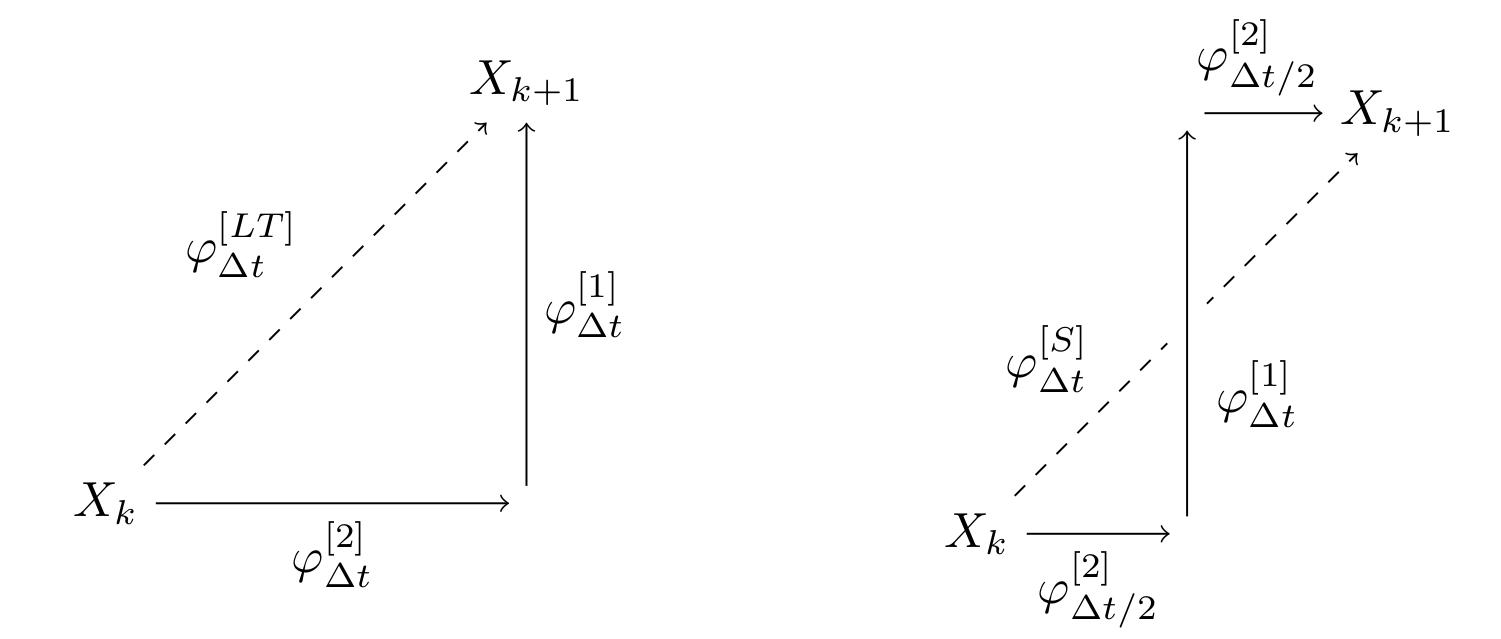
\includegraphics[scale = .185]{figures/strangAndLieTrotter.jpeg}
    \end{center}
    \caption{A diagram of the Lie-trotter- (left) and Strang (right) compositions}
    \label{figure:StrangAndLieTrotterPlot}
\end{figure}\\
Although they are quite similar overall, the one-step predictions of the transition densities given by the Strang splitting scheme is proven to be superior to that of LT; compare \cite[Proposition 3.4 and 3.6]{SplittingSchemes}. For this reason, we only consider the Strang splitting scheme but our ideas could very easily be adapted to Lie-trotter schemes. We start by looking at the Strang splitting on a general one-dimensional SDE with additive noise. Later we comment on the possible ways to use this method even for models with multiplicative noise.\\
\textbf{Models with additive noise}\\
General one-dimensional autonomous stochastic differential equations with additive noise can be written as
\begin{align}
    \mathrm{d}X_t = b(X_t; \theta)\mathrm{d}t + \sigma\mathrm{d}W_t, \label{eq:generalAdditiveNoiseSDE}
\end{align}
note that we have highlighted the dependence of some parameter, $\theta\in\Theta\subseteq\mathbb{R}^p$ in the drift. When we have additive noise, splitting schemes work by decomposing the process into a linear SDE and a non-linear ODE in the following way
\begin{align}
    \mathrm{d}X_t^{(1)} &= -\beta(\theta)\left(X_t^{(1)} - \mu(\theta)\right)\mathrm{d}t + \sigma \mathrm{d}W_t, &&X_t^{(1)} = x_0, \label{SDE_split}\\
    \mathrm{d}X_t^{(2)} &= N\left(X_t^{(2)}; \theta\right)\mathrm{d}t, &&X_t^{(2)} = x_0, \label{ODE_Split}
\end{align}
where the splitting is constructed such that the sum of (\ref{SDE_split}) and (\ref{ODE_Split}) is equal to (\ref{eq:generalAdditiveNoiseSDE}), meaning that $N$ is some non-linear defined as the difference between the drift in (\ref{eq:generalAdditiveNoiseSDE}) and (\ref{SDE_split}). Evidently, this splitting is not unique, and thus the way we construct the estimator will not be either. However, it turns out that any splitting of (\ref{eq:generalAdditiveNoiseSDE}) done in this way yields approximations of the transition densities that are equivalent asymptotically \cite{{SplittingSchemes}}. Yet, our choice might have an impact on the quality for finite samples. Additionally, in practice it is not difficult to imagine that some splittings are numerically more well-behaved than others. So we still have to carefully consider our splitting choice. The one we use for the most part is the heuristic provided in \cite[section 2.3 and 2.5]{SplittingSchemes}. The strategy presented here is: Construct (\ref{SDE_split}) as the linearization around the fixed points of the drift. This means, we use $b(X_t, \theta)$ from (\ref{eq:generalAdditiveNoiseSDE}) and solve the following equation
\begin{align}
     b(X_t; \theta) = 0,
\end{align}
in terms of $X_t$. Then set $\mu\left(\theta\right)$ to be equal to this solution and plug the value into the derivative of $b(X_t, \theta)$ w.r.t. $x$
\begin{align}
    \beta\left(\theta\right) = \left.\frac{\partial b(x; \theta)}{\partial x}\right|_{x = \mu\left(\theta\right)}.
\end{align}
The two components is used together to construct (\ref{SDE_split}).
Hereafter, (\ref{ODE_Split}) is calculated as the residual of the \ref{eq:generalAdditiveNoiseSDE} and our (\ref{SDE_split}). 

Recall that in the one dimensional case, the solution with stepsize, $\Delta t$, to the linear SDE is given by the flow
\begin{align}
    \varphi_{\Delta t}^{(1)}(x) = \exp\left(-\beta\left(\theta\right) \Delta t\right)\left(x - \mu\left(\theta\right)\right) + \mu\left(\theta\right) + \xi_{\Delta t}, \label{varphiTheoretical}
\end{align}
with $\xi_{\Delta t}\sim\mathcal{N}\left(0, \Omega_{\Delta t}\right)$. That is, the flow is gaussian with mean and variance
\begin{align}
    \mu_{\Delta t}(x; \theta) &= \exp\left(-\beta\left(\theta\right) \Delta t\right)\left(x - \mu\left(\theta\right)\right) + \mu\left(\theta\right) \label{linearSDEMean}\\
    \Omega_{\Delta t} &= \frac{\sigma^2}{2\beta}\left(1 - \exp\left(-2\beta\left(\theta\right)\Delta t\right)\right), \label{linearSDEVariance}
\end{align}
which we calculated in (\ref{eq:OU_solution}). For our purposes the solution to (\ref{ODE_Split}) exists and is unique; this is ensured by the Picard-Lindelöf theorem \cite[section 2.7]{Srkk2019}, since (\ref{ODE_Split}) is ordinary differential equations that in our case will be sufficiently regular for the assumptions from the theorem to hold. Still, we might find ourselves in a situation, where we cannot get a closed form solution to (\ref{ODE_Split}), simply due to the complexity of the ODE. In those cases, we use the Fourth Order Runge-Kutta method to solve it numerically \cite[p.541 equation (8)]{numericalAnalysis}.  
Nevertheless, we denote the solution with stepsize, $\Delta t$, $\varphi_{\Delta t}^{(2)}$. By figure \ref{figure:StrangAndLieTrotterPlot} the Strang splitting scheme then gives the approximation of the transition density as 
\begin{align}
    X_{t_{i+1}}^{(S)} = \varphi_{\Delta t / 2}^{(2)}\left(\mu_{\Delta t}\left(\varphi_{\Delta t/2}^{(2)}\left(X_{t_{i}}^{(S)}\right); \theta\right) + \xi_{\Delta t} \; ; \theta \right). \label{eq:classicStrangSplitting}
\end{align}
Due to the fact that (\ref{varphiTheoretical}) is gaussian, (\ref{eq:classicStrangSplitting}) is a non-linear transformation of a gaussian variable with the specified mean and variance. So by the density transformation theorem, this flow has the following negative pseudo-loglikelihood 
\begin{align}
    l^{[S]}(\mathbf{x}; \theta) &= -\sum_{i = 0}^{N - 1}\log\left(g\left(\left(\varphi_{\Delta t / 2}^{(2)}\right)^{-1}\left(x_{t_{i+1}}\right); \mu_{\Delta t}\left(\varphi_{\Delta t/2}^{(2)}\left(x_{t_{i}}\right); \theta \right), \Omega_{\Delta t} \right) \right) \nonumber \\
    &- \sum_{i = 0}^{N - 1}\log\left(\frac{\partial}{\partial x}\left(\varphi_{\Delta t / 2}^{(2)}\right)^{-1}\left(x_{t_{i + 1}}\right) \right), \label{eq:Strang_likelihood}
\end{align}
where $t_N$ is the index of the most recent sample in the data. (\ref{eq:Strang_likelihood}) is the Strang based pseudo-likelihood, and we say that the $\theta$ that minimizes this function is the Strang-based estimator. In (\ref{eq:Strang_likelihood}) $g$ is the gaussian density function with the specified mean and variance. 
To get the inverse of the solution to the ODE, we use the property $\left(\varphi_{\Delta t}^{(2)}\right)^{-1} = \left(\varphi_{-\Delta t}^{(2)}\right)$ \cite[Remark below equation (9)]{SplittingSchemes}, and solve the resulting ODE analytically or with the fourth-order Runge-Kutta. Finally, to get the derivative we use direct computation when possible and Richardson extrapolation, if we used the Runge-Kutta method before. For a differentiable function, $f$, a simple Richardson extrapolation approximates the derivative as
\begin{align}
    f'(x) = \frac{f(x + h) - f(x - h)}{2h}, \qquad h > 0,
\end{align}
with an error that is $\mathcal{O}(h^2)$. It is possible to repeatedly use Richardson extrapolation to get even higher-orders of accuracy. However, for our purposes this simple approximation suffices.
\\\\
\textbf{Models with multiplicative noise}\\
As noted we require additive noise in the models. This is specifically because the method hinges on the fact that (\ref{SDE_split}) is an Ornstein-Uhlenbeck process of which we have a simple known solution. There are, of course, many interesting models that do not have additive noise such as five of six model in table \ref{table:ergodicDiffusions}. But as we have already clarified, all of these processes are reducible and as such we can transform the processes with the lamperti-transform (\ref{eq:lampertiDefinition}) to get additive noise; and then do the estimation on the resulting SDE in the exact manner as described above. This procedure is the one proposed in \cite{SplittingSchemes}, for which there exist theoretical results on the accuracy of the transition density. It is also the way we mostly use the Strang splitting.\\\\
Still, we consider different options. As an alternative, we use the same splitting philosophy as \cite{SplittingSchemes}, but leave the noise as it is. This, of course, means that the linear SDE inherits the multiplicative noise from the original SDE. However, other methods for estimation in stochastic differential equations exist and we can then use those on the linear SDE in the splitting. We went with Kessler's method, which assumes a gaussian transition density, but uses the true conditional mean- and variance \cite[equation (1.7)]{Kessler1997}. Even still, there is another possibility. In a few cases there exists closed form solutions to other linear stochastic differential equations than the one with additive noise. This splitting strategy avoids using the Lamperti-transform, while still using exact solutions to the SDE in the splitting. \\\\
Although, the last two types of splittings are not central to the estimation of the AMOC, we still illustrate them as they present alternative ways of using the Strang splitting scheme to construct pseudo-likelihoods. A concrete derivation for the latter option can be seen in (\ref{meanrevertingGBMSplit1}). Note that in this example, we must use a different splitting than the heuristic provided by \cite[section 2.3 and 2.5]{SplittingSchemes}, because the solution of the stochastic differential equation in the example only exists on closed-form, whenever $\mu(\lambda) = 0$. We would have to be quite fortunate to have the fixed point equal 0; thus this splitting strategy rarely aligns with the heuristic from the paper.
\subsubsection{Approximately Optimal Martingale Estimation Equations}\label{subsubsec:approximatelyOptimalMartingaleEstimationEquation}
Other than the strang splitting, we also estimate the parameters by means of approximately optimal martingale estimation functions (AOMEF). As a means of estimation these are conceptually different from what we have done thus far; with them our aim is not to approximate the transition density, but instead construct functions where the estimator is defined as a solution to a system of equations similarly to how a score function (\ref{eq:transitionScore}) normally is used. Not surprisingly, AOMEF's are based on the notion of an martingale estimaton equation. The theory behind these is quite involved measure-theoretically, for which reason we only summarize the most important ideas in their construction. We assume that we want to estimate the parameters, $\theta\in \Theta \subseteq \mathbb{R}^p$ and $\sigma$, in a one-dimensional stochastic differential equation such as (\ref{eq:SDEInference}); and say that the solution to this equation has state space, $D\subseteq \mathbb{R}$. Furthermore, let $p(x, y, \Delta t; \theta)$ be the transition density of $X_{t+\Delta t}$ given $X_t$, evaluated at the point $y$. Then a martingale estimation function is 
\begin{align}
    G_N(\theta) = \sum_{i = 1}^N g(X_{t_{i - 1}}, X_{t_i}, \Delta t; \theta), \label{eq:estimationEquation}
\end{align}
where $g$ is some function such that
\begin{align}
    \int_{D} g(x, y, \Delta t; \theta)p(x, y, \Delta t; \theta)\mathrm{d}y = 0. \label{eq:martingaleProperty}
\end{align}
In other words, $G_N$ is a martingale w.r.t. the filtration $\mathcal{F}_n = \sigma\left(X_{t_i}; i \leq n\right)$. \cite[p. 11]{StatisticalMethodsForSDE} establishes that an example of such an equation is the score equation. This can easily be seen by inserting (\ref{eq:transitionScore}) in (\ref{eq:martingaleProperty}). In this way the martingale equations can be seen as a generalization of the score equation. Now, we know that the solving the score equation yields the maximum likelihood estimator; an estimator with many desirable properties. Thus, we are interested in picking a function, $g$, satisfying (\ref{eq:martingaleProperty}) that is optimal in the sense that it approximates the score well. We do this by taking a collection of real valued functions $h = (h_1, \dots, h_m)^\top$, where each individual function satisfies (\ref{eq:martingaleProperty}) and choose $g$ in (\ref{eq:estimationEquation}) so
\begin{align}
    G_N(\theta) = \sum_{i = 1}^N a\left(X_{t_i}, \Delta t, \theta \right)h(X_{t_{i - 1}}, X_{t_i}, \Delta t; \theta), \label{eq:estimationEquationWeight},
\end{align}
where $a$ is a $p\times m$-matrix that is a function that (\ref{eq:estimationEquationWeight}) is integrable w.r.t. $P_\theta$. Therefore (\ref{eq:estimationEquationWeight}) is a martingale, because the $h_j$ satisfy (\ref{eq:estimationEquation}). The $h$-functions are often chosen such that
\begin{align}
    h_j = f_j(X_i, \Delta t) - \mathbb{E}_\theta\left[f_j(X_i)| X_{t_{i - 1}} = x_{t_{i - 1}}\right].
\end{align}
The specific $h$-functions, we consider, are
\begin{align}
    h_1(x,y, \Delta t; \theta) &= y - \mathbb{E}_\theta\left[X_{t_i + \Delta t} \middle| X_{t_{i}} = x\right] \\
    h_2(x,y, \Delta t; \theta) &= \left(y - \mathbb{E}_\theta\left[X_{t_i + \Delta t} \middle| X_{t_{i}} = x\right]\right)^2 - \mathrm{Var}\left[X_{t_i + \Delta t} \middle| X_{t_{i}} = x\right],
\end{align}
For typographical reasons denote the conditional mean and -variance, $F$ and $\Phi$, respectively, in the following.
 We use the estimation function based on the quasi-score function of a gaussian transition density \cite[equation (1.28)]{StatisticalMethodsForSDE}. This corresponds to using the weight matrix
 \begin{align}
    \left(\frac{\frac{\partial}{\partial\theta}F(\Delta t, x;\theta)}{\Phi\left(\Delta t, x; \theta\right)} , \frac{\frac{\partial}{\partial\theta}\Phi(\Delta t, x;\theta)}{2\Phi^2(\Delta t, x;\theta)\Delta t} \right),
\end{align}
in (\ref{eq:estimationEquationWeight}) along with the $h$-functions from before. It turns out that for small enough $\Delta t$, these weights are a good approximation of the actual optimal weights \cite[equation (1.32)]{StatisticalMethodsForSDE}, which can be much more complex.\\\\
Finally by \cite[lemma 1.10]{StatisticalMethodsForSDE} the weight can be simplified to
\begin{align}
    \left(\frac{\frac{\partial}{\partial\theta}b(\Delta t, x;\theta)}{\sigma^2\left(\Delta t, x; \theta\right)} , \frac{\frac{\partial}{\partial\theta}\sigma^2(\Delta t, x;\theta)}{2\sigma^4(\Delta t, x;\theta)\Delta t} \right),
\end{align}
This gives us the estimation equations for one-dimension stochastic differential equations that \cite[Example 1.11]{StatisticalMethodsForSDE} also arrives at
\begin{align}
    G_N^{\circ} &= \sum_{i = 1}^N 
    \left(
        \frac{\frac{\partial}{\partial\theta} b\left(X_{t_{i-1}};\theta\right)}{\sigma^2\left(X_{t_{i-1}};\theta\right)}
    \right) \left(X_{t_{i}} - \mathbb{E}\left[X_{t_{i}} \middle| X_{t_{i-1}} = x\right]\right) \nonumber \\
    &+ \frac{\frac{\partial}{\partial\theta}\sigma^2\left(X_{t_{i-1}}; \theta\right)}{2\sigma^4\left(X_{t_{i - 1}}; \theta\right)\Delta t}\left(\left(X_{t_{i}} - \mathbb{E}\left[X_{t_{i}} \middle| X_{t_{i-1}} = x\right]\right)^2 - \textrm{Var}\left[X_{t_{i}} \middle| X_{t_{i-1}} = x\right]\right),\label{eq:approximatelyOptimalMartingale}
\end{align}
and even with the numerous assumptions and simplifications made thus far, this approximately optimal martingale estimation equation still gives a consistent estimator of $\theta$ \cite[p.19]{StatisticalMethodsForSDE}. In appendix \ref{sec:AppendixEstim} we derive estimators that are based on these methods for two of the Pearson diffusions.
\subsubsection{Parameter estimation in the stochastic normal form}
We now switch our attention to the concrete estimation and present the estimators that we use on (\ref{eq:standardStochasticForm}). Firstly, as the two forms in our models only differ by the sign in front of drift, we just carry the negative in the parameters $A$ and $\lambda_0$, whenever we want to estimate in positive branch of the model. Having a scaling-coefficient, $A$, which is negative is of course odd, but this is merely such that we can use the same methods for both versions of (\ref{eq:standardStochasticForm}). That is we always interpret $A$ and $\lambda_0$ as positive and negative, respectively.\\\\
As in \cite{Ditlevsen2023} split (\ref{eq:standardStochasticForm}) into two parts. What we will refer to as the stationary part and the dynamic part. This corresponds to the time before and after ramping starts, i.e. before and after $t_0$, respectively. The estimation we do depends on which part we are in and it is done sequentially. That is, we need the estimates from the stationary part to do estimation in the dynamic part. For ease of notation we assume that we have have uniform temporal resolution. \\\\
\textbf{Estimation in the stationary part of the processes}\\
Regardless of the specific noise term from table \ref{table:ergodicDiffusions}, we use the same overall procedure. At times before ramping, i.e. $t < t_0$, our models is governed by
\begin{align}
    \mathrm{d}X_t = -\left(A(X - m)^2 + \lambda_0\right)\mathrm{d}t + \sigma\sqrt{\left(aX_t^2 + bX_t + c\right)}\mathrm{d}W_t, 
\end{align}
A Taylor-expansion of the drift around the fixed point \ref{eq:fixedPoint} gives
\begin{align}
    \mathrm{d}X_t = -\alpha_0\left(X_t - \mu_0\right)\mathrm{d}t + \sigma\sqrt{\left(aX_t^2 + bX_t + c\right)}\mathrm{d}W_t, \label{eq:TaylorStationary}
\end{align}
where $\alpha_0 = 2\sqrt{-\lambda_0 A}$ and $\mu_0 = m + \sqrt{-\frac{\lambda_0}{A}}$.\\\\
We then estimate the parameters $\theta_{\mathrm{stationary}} = (\alpha_0, \mu_0, \sigma)^\top$ with the samples, $x_{0}, \dots, x_{t_0}$, from the stationary part of the process. Depending on the stochastic term, this could be done through Strang-based estimators, approximately optimal martingale estimation equations or even maximum likelihood estimation. We present an overview of the estimators and where one can refer to for their derivations, when we have discussed estimation in the dynamic part of the processes.\\
\textbf{Estimation in the dynamic part of the processes}\\
In their dynamic part the approximation from the Taylor-expansion of the dynamics is no longer adequate to do inference with as the dynamics are too non-linear. We assume we have samples $x_{t_0+\Delta t}, \dots x_{N}$ from the process, $X_t$, that solves the following SDE
\begin{align}
    \mathrm{d}X_t = -\left(A(X_t - m)^2 + \lambda_t\right) + \sigma\sqrt{\left(aX_t^2 + bX_t + c\right)}\mathrm{d}W_t, 
\end{align}
and because $t>t_0$
\begin{align}
    \lambda_t = \lambda_0\left(1 - \frac{t - t_0}{\tau_c}\right)^\nu, \qquad \nu >0.
\end{align} 
In our implementation we need to evaluate $\lambda_t$ between points, so for computational efficiency and easy of implementation we assume that it is constant between observations. For fine temporal resolutions this approximation is obviously rather good as $\lambda_t$ is smooth. A solution to this in a coarser setting could be to linearly interpolate the values of $\lambda_t$ between consecutive observations; though, we do not pursue this option here. 

Instead, see that given $\theta_{\mathrm{stationary}}$, we only need to estimate $\theta_{\mathrm{dynamic}} = (A, \tau_c, \nu)$, The remaining parameters we get by using the relations given by the first-order Taylor expansion of the stationary part: $\lambda_0 = -\frac{\alpha_0^2}{4A}$ and $m = \mu_0 - \frac{\alpha_0}{2A}$ as plug-in estimators. We exclusively use Strang-based estimators for the estimation of $\theta_{\mathrm{dynamic}}$. 
\subsubsection{Overview of all estimators}
We are now ready to present the estimators we use. For sake of brevity we use this section to present a small table with the estimates that we use for each model and references to where derivation for them can be found in the appendix.
\begin{table}[h!]
    \centering
    \begin{tabular}{llll}\hline
    \textbf{Model} & \textbf{Stationary part} & \textbf{Dynamic-} & \textbf{References}\\ \hline
    OU & MLE & Strang & \cite[equation (S3), (S9-S10)]{DitlevsenSupplementary} \\
    Square-root & AOMEF, Strang & Strang\textsuperscript{2} & (\ref{eq:squarerootMartingaleEquation}, \ref{eq:squarerootStationarySplit1}) and (\ref{eq:squareRootSplit1}, \ref{eq:lampertiSquarerootSplitting1})\\
    Linear & AOMEF, Strang\textsuperscript{2} & Strang\textsuperscript{2} & (\ref{eq:GBMapproxOptimalMartingaleEstimationEquation}, \ref{meanrevertingGBMSplit1}, \ref{eq:GBM_LinearSDE_split}) and (\ref{eq:GBMSplit1}, \ref{eq:GBMLampertiBasedStrang}) \\
    Skew t-diffusion & Strang & Strang & \ref{eq:StrangTDiffusion} and \ref{eq:StrangTDiffusionDynamic}\\
    Scaled F-diffusion & Strang & Strang & \ref{eq:scaledFStrang} and \ref{eq:dynamicScaledFLamperti}\\
    Jacobi-diffusion & Strang & Strang & \ref{eq:JacobiLampertiSDE} and \ref{eq:JacobiLampertiDynamicSDE}\\
    \hline
    \end{tabular}
    \caption{Overview of the estimators.}
    \label{table:Estimators}
\end{table}\\
Note that in table \ref{table:Estimators} Strang with a superscript denotes multiple applications. The references in "References"-column are given in the order left-to-right the estimators appear in the table. And the "Model"-column naturally refers to the what diffusion term in table \ref{table:ergodicDiffusions} that is used in (\ref{eq:standardStochasticForm}).
\subsection{Numerical Optimization in \code{R}}
Numerical optimization is central in applications of machine learning and statistics. For almost all of the estimators in table \ref{table:Estimators} some form of numerical optimization takes place. In this section, we mention the methods that we use and some motivation for the choices that was made. Also, we introduce a numerical Strang-based negative log-likelihood based on the heuristics of \cite{SplittingSchemes}. Note that model-specifics such as choice of starting values are commented on in the individual estimation methods. 

We opted for the \code{R}-language \cite{Rlang}, because of its rich ecosystem for numerical optimization. \code{R} has a bad reputation in terms of computation speed. However, it actually offers many easy to use abstractions of highly optimized \code{C} and \code{C++} code that if used properly lets us harness the speed of compiled code. 
\subsubsection{General optimization and implementation}
For each part of the process, i.e. before and after ramping begins, we optimize a bit differently. Because of this, we have implemented two wrappers around {stats::optim} \cite{Rlang}. Each of which is implemented such that they can be invoked with any likelihood function, we have implemented for that part. In addtion, we allow any valid \code{stats::optim}-argument to be called in both wrappers. This is especially useful, because the arguments to \code{stats::optim} can vary depending on the specific algorithm, one wishes to use. Also, since \code{stats::optim} uses an ellipsis, our wrappers does too. That is, our wrapper can pass on any argument directly onto \code{stats::optim}. This is for example useful, if we have objective functions with special arguments that we would like to use in the optimization.

Still, the wrapper obviously has to have a couple of default arguments to make it easier to use. For instance, both parts use the built-in BFGS optimization algorithm, due to its robustness. Though, as said we could specify any other optimization algorithm implemented in \code{stats::optim} during the call. Furthermore, we implement a \code{return\_all}-argument that lets us control whether we want to just return the objective and parameters after optimization or all of the objects from \code{stats::optim}.

For the dynamic part, we need to provide the values for $\alpha_0, \mu_0, \sigma$. This the ellipsis-construct seemingly allows us to do. Of course, the values we pass on here are the estimated values of these from the stationary part of the processes. In addition, the optimizer of the dynamic part dynamically chooses to estimate the $\nu$-parameter dependending on the dimension of the initial values that we provide. If the dimension is two, we implicitly assume $\nu = 1$, while a dimension of three allows the optimizer to estimate it. Throughout the implementations stability of the objective functions is something we are greatly concerned with. 

Firstly, we have quite a few formulas containing $\exp\left(x\right) - 1$ or its additive inverse in our applications. One example of this is in the variance of the Ornstein-Uhlenbeck (\ref{linearSDEVariance}). For small $\Delta t$ arguments of the exponential function is this example can be quite close to zero, and thus we need to take care in order to avoid catastrophic cancellation. Luckily, others have had this problem before us, and we make use of the \code{base::expm1} method in \code{R} that calls the \code{C}-function of the same name - a method optimized for this very problem. \cite{cppreference_expm1} If we do not do this, our program might crash or give misleading estimates. In the case of (\ref{linearSDEVariance}) for instance, we risk having a variance of zero, due to catastrophic cancellation. While methods in \code{R} such as \code{stats::dnorm} allow the use of this degenerate distribution, we are of course not interested in such a transition density.

Secondly, to ensure numerical stability we also use as many pre-implemented methods as possible. This includes \code{stats::dnorm} with \code{log = TRUE} for the log-likelihood of a gaussian random variable. Abstracting some of the computations away we avoid making mistakes in the implementation and methods that are in \code{R} by default are generally robust and relatively fast.
\subsubsection{A numerical Strang method in \code{R}}\label{subsection:NumericalStrangSplitting}
In this section, we briefly describe an almost entirely numerical Strang splitting scheme based estimator with the splitting philosophy presented in \cite{SplittingSchemes}. Deriving expression of estimators of stochastic differential equations is a quite error prone process. We have already limited the amount of errors we can make somewhat by relying on the Fourth-Order Runge-kutta method to solve differential equations in some of the versions of the Strang splittings. However, we mostly did this due to the fact that closed form solutions to some of the differential equations simply were to difficult to derive. Further limiting the amount of manual computations could decrease the amount of error we make. Of course, it is more difficult to implement such a method in the first place as the program must take care of the things, it previously could take as given.

Nevertheless, we implemented a method where the only thing we need to provide is the Lamperti-transform and the drift of the SDE that comes by applying Ito's formula to the lamperti transform. Calling the wrapper with this objective function, where we pass onto the it the lamperti-transformed drift and - data and the implementation takes care of the rest. Under the hood the method works the same as the less automated versions with regards to solving the ordinary differential equations - that is it solves them with a fourth-order Runge-Kutta. However, the construction of (\ref{SDE_split}) and (\ref{ODE_Split}) is different. The latter is of course just computed as the residual of lamperti-transformed drift that we pass to the method and the linear SDE. With regards to the linear SDE, however, the method only has the heuristic that it needs to construct the SDE as the linearization around the fixed point of the drift as a requirement. To find the fixed point numerically, we use the method \code{nleqslv::nleqslv}; an efficient method implemented in \code{Fortran} that finds zeroes with Newton's method \cite{nleqslv}. This method needs an initial guess for the fixed point, for which the median of the lampert-transformed data is natural for our purposes. The method then computes the derivative of the drift numerically with \code{numDeriv::grad}, which uses highly optimized finite difference methods \cite{numDeriv}. We plug the fixed point into this function to get the slope for the linearization, and the remaining construction is done analagously to earlier.
\subsection{Model assessment}
For this part, we briefly introduce the metrics used for evaluating the quality of our estimators in a simulation setting. Additionally, we show the method that we use to diagnose the fit of a particular method to data, and how we contruct confidence intervals for the estimators.
\subsubsection{Diagnostics and confidence intervals}
When we are in a simulation setting, we assess our estimation methods using the absolute relative error. With sample size $N$, this is for the $i$th-coordinate in our parameter vector defined as
\begin{align}
    \mathrm{ARE}\left(\theta_N^{(i)}\right) = \frac{\left|\theta_N^{(i)} - \theta^{(i)}\right|}{\theta^{(i)}}. \label{eq:ARE}
\end{align}
Of course, we are not able to calculate this quantity when we do not have access to the ground-truth parameters, so it is only relevant in a simulation setting In addition, we cannot use regular residuals to diagnose the fit, as each data point have different distributions depending on the previous point. Instead, we assess the fit qua so-called uniform residuals. These are constructed using the transition density, $p_\theta(x|\Delta t, x_0)$. Though, as is quite clear by now, this is rarely something we can compute. However, we can for instance use the approximation given from the Strang scheme in its stead. As this also gives us an approximation for the conditional distribution function, $F_\theta(x|\Delta t, x_0)$, and as $F_\theta(X_{t_{i}}|\Delta t, X_{t_{i - 1}})\sim \mathrm{Unif}(0,1)$ if $X_{t_{i}}|X_{t_{i - 1}} \sim p_\theta$. Still, it is sometimes difficult to detect outliers in the uniform distribution, so we introduce another transformation - this time with the quantile function of the standard gaussian distribution. Then by the quantile transformation theorem, the double-transformed samples should follow a standard gaussian, if the model is properly specified. To see whether this is the case, we use ordinary QQ-plots.\\\\
As the approximately optimal martingale estimation functions approximate the score function, we do not have any approximation of the transition density here and cannot use uniform residuals. Even still with some creativity, we can do diagnostics, but only of the square-root process. If we let $X_t$ be governed by the square-root process, then
\begin{align}
    Y_{t_{i + 1}} := \frac{4\alpha_0}{\sigma^2\left(\exp\left(-\alpha_0 \Delta t\right) - 1\right)}X_{t_{i + 1}}
\end{align}
has transition density of a non-central $\chi^2$-distribution with $\frac{4\alpha_0\mu_0}{\sigma^2}$ degrees of freedom with non-centrality parameter $Y_{t_k}\exp\left(-\alpha_0 \Delta t\right)$ \cite[Equation (5.68)]{Srkk2019}. For the other diffusions, we do not have an analagous property to exploit, and we may only assess the martingale estimation equation based estimators by ensuring that the estimates are consistent with methods based on the transition density, where we can use uniform residuals.\\\\
Finally note that we obviously have no hope of knowing the distribution of our estimators. Therefore to get an idea of our uncertainty of them, we use parametric bootstrap. That is, for a specific model we estimate its parameters from data. Then we sample from that model repeatedly using the parameters we estimated on the real data and estimate parameters on these artificial data sets. The distribution of the estimates achieved in this way then gives us the quantiles etc. for our estimator.
\section{Simulation study}\label{Simulaton study}
As said in section \ref{subsubsec:Discretization} the simulations are done with the Scalar-weak order 2.0 Itō-Taylor method \cite[algorithm 8.5]{Srkk2019}. The concrete schemes that we derived for the respective types of noises are shown in equations (\ref{eq:OUSim} - \ref{eq:jacobiDiffusion}). All the schemes are implemented in \code{R} and they can be called with specific parameter choices, values for $\tau_c$ and $t_0$ as well as a temporal resolution, $\Delta t$,  and starting point, $x_0$. 

Depending on the $\tau_c$, $t_0$, and $\Delta t$ the method dynamically picks the appropriate number of samples to draw for $\Delta W_k\sim\mathcal{N}\left(0,\Delta t\right)$. The methods allow for positive $\lambda_0$ and negative $A$, but recall that this only corresponds to choosing between the positive and negative versions of (\ref{eq:standardStochasticForm}). If no starting point is specified the method picks the fixed point in the stationary part of the process as the starting point; note that this of course is done with the appropriate branch of (\ref{eq:fixedPoint}) depending on the version of (\ref{eq:standardStochasticForm}), i.e. the sign of $A$. Additionally, an argument is implemented such that we can opt for stopping the process at earlier time (or later) points in time than $\tau_c$. This is useful when we want to evaluate the models' ability to predict the tipping point based on how far from it we have samples. For details about the timing benchmarks refer to section \ref{section:benchmark}. Specifications on hardware and software used can be found in Table \ref{tab:specs}. 
\subsection{Overview of the Estimation methods}
In this section, we test our methods on simulated data. The test aims to illustrate the robustness, computational efficiency and precision in terms of ARE (\ref{eq:ARE}) of the estimation methods. To perform the study for all the models and their respective methods at once, we draw sample paths with the parameters that worked for all models in Figure \ref{figure:samplesFromAllDifferentModels}. That is $A = 1.5, m = 0.4, \lambda_0 = -0.2, \sigma = 0.1$; in this part, we let $\nu = 1$ and do not estimate this parameter for now. According to the first-order Taylor expansion, which we use in the stationary part (\ref{eq:TaylorStationary}), the true values here are, $\theta_{\mathrm{stationary}} = (1.095, 0.7651, 0.1)^\top$. We simulate using $t_0 = 30$ and $\tau_c = 30$ as well as temporal resolutions $\Delta t = \{1/5, 1/10, 1/25, 1/100, 1/250\}$, corresponding to $N = \{150, 300, 750, 3000, 7500\}$ number of samples in each part of the process. For each value of $N$, we run the simulations and estimation $M = 50$ times and record the median ARE for each parameter. In addition, we calculate the median run-time for each method. In both cases we use the median due to it being more robust against outliers than the mean.

Furthermore, due to the possibility of extreme samples for small $N$; we implement a \code{trycatch}-wrapper around the estimation part such that the program fails gracefully if estimation should somehow be infeasible for a model on a specific sample. For each run in the simulation all the models are simulated with the same realizations of the Brownian motion; if one model fails all models are re-run using a new seed. The optimizers are initialized at random points where each coordinate can deviate up to $\pm 10\%$ at random from the true values; this is done by sampling three uniform variables according to $U\sim\mathrm{Unif}(0.9, 1.1)$ and multiplying them with the true values. As convergence criterion for the likelihood-based methods we use a relative tolerence of $\code{sqrt(.Machine\$double.eps)/10}\approx 1.49\cdot 10^{-9}$, while the estimation equations that solves their equation numerically use $10^{-8}$ the standard of \code{nleqslv::nleqslv}. \\\\
The likelihood-based methods are the MLE and the Strang-based estimators; when there is more than one such method for a specific model, we denote it \textit{Likelihood (Alt.)}. Naturally, we use the common term \textit{Estimation equation}-based estimator to refer to estimators based on the score equation or martingale estimation equations.
\subsubsection{The Stationary parts}
In the stationary parts, we run the simulations as described above and depict the median ARE as a function of sample size on a double logarithmic scale
\begin{figure}[h]
    \begin{center}
    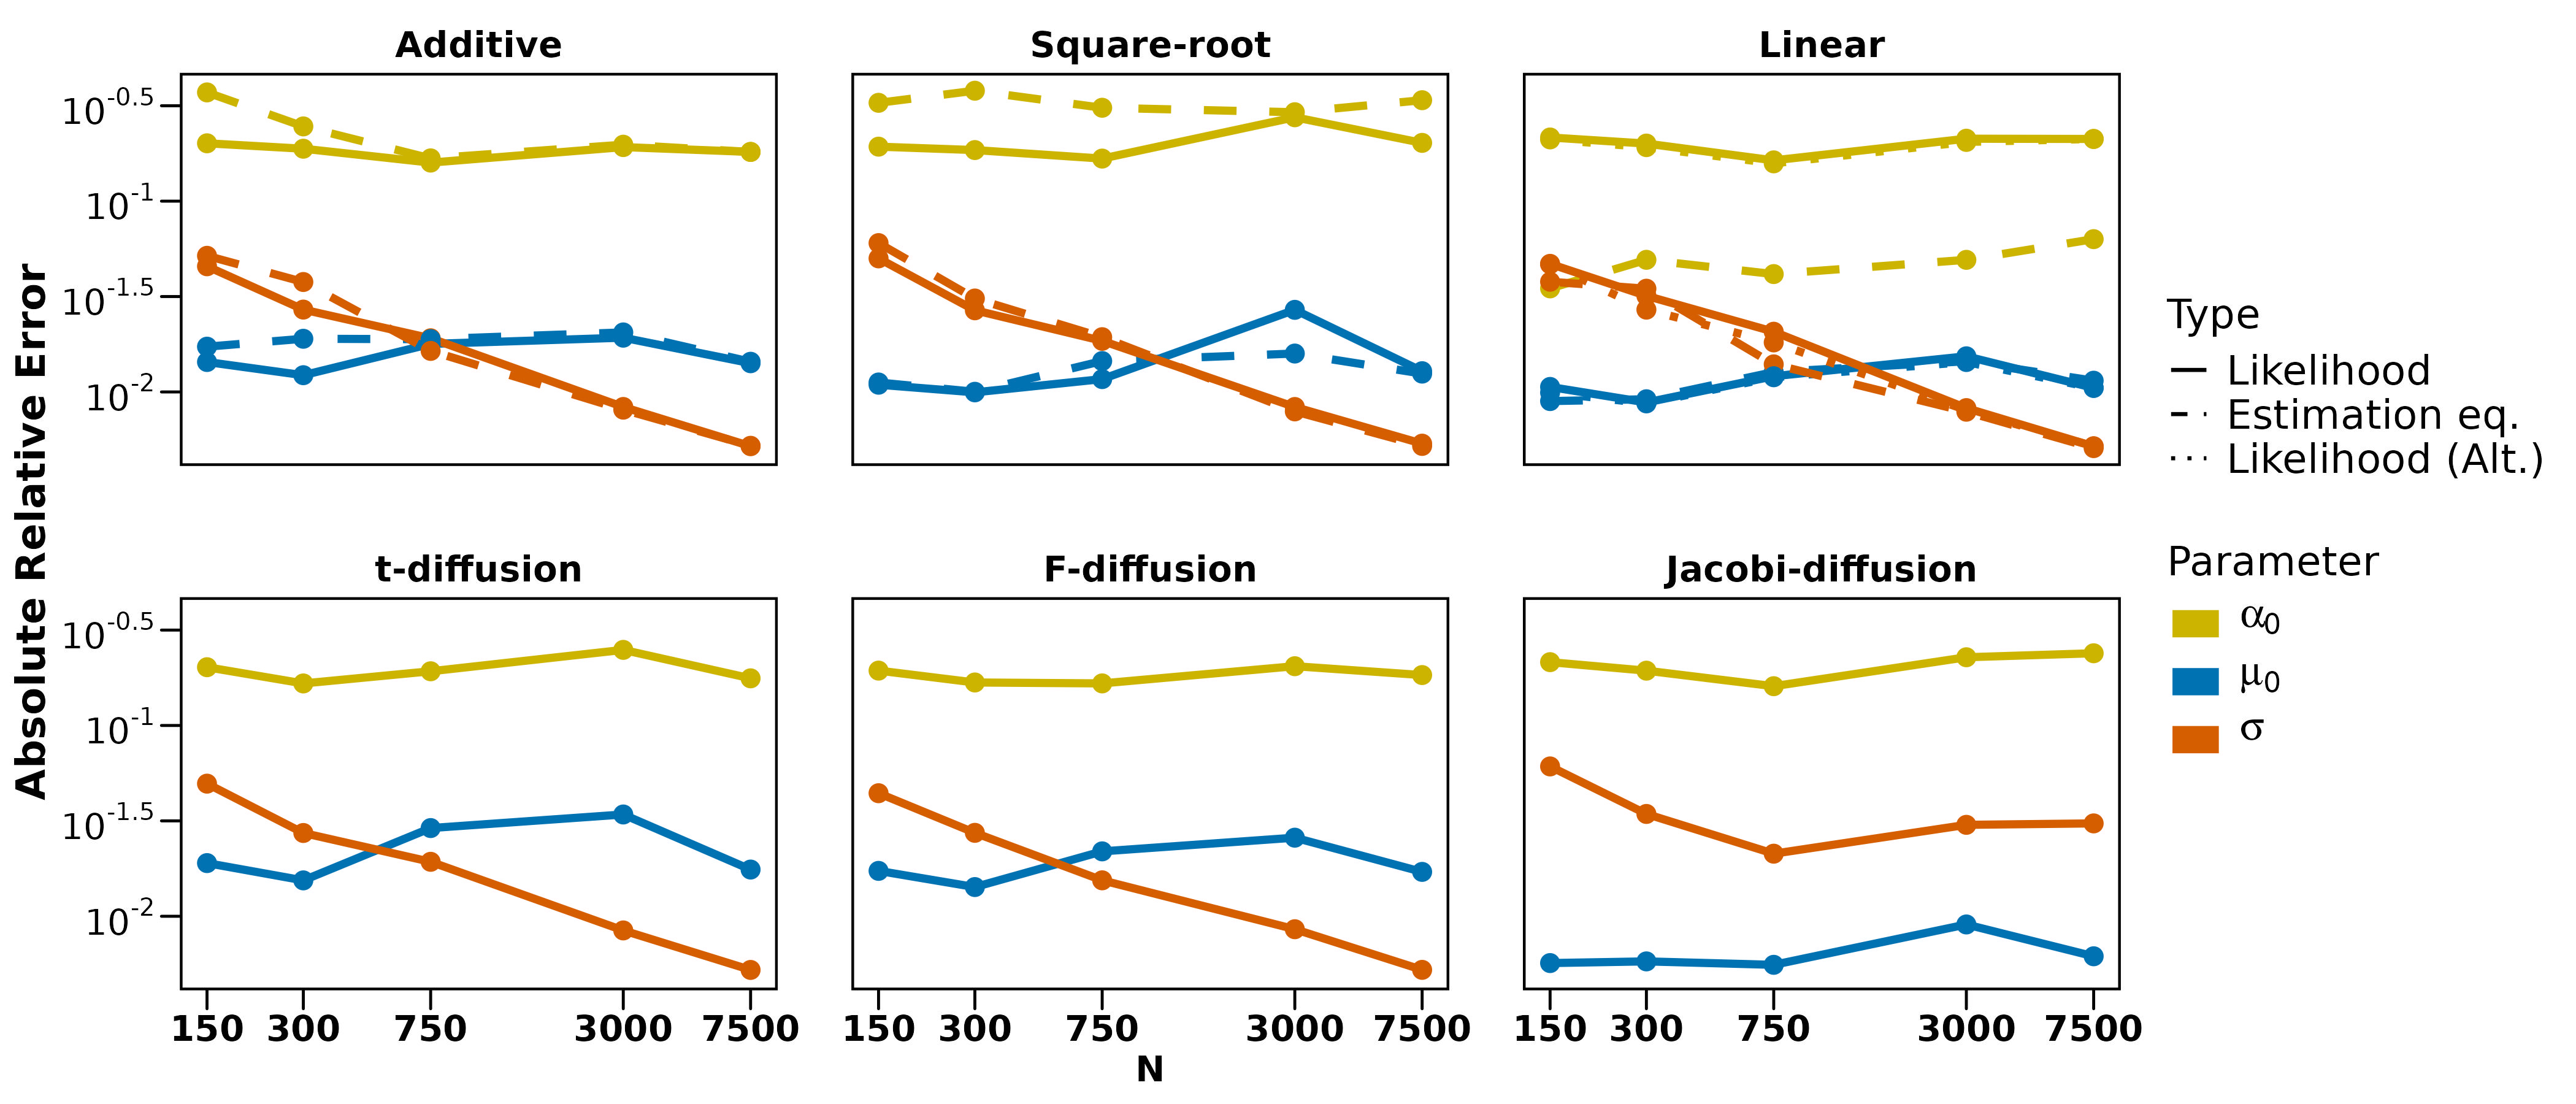
\includegraphics[scale = .1]{figures/parameter_precision_stationary.jpeg}
    \caption{Overview of our estimation methods for the stationary parameters applied to the models}
    \label{figure:overviewOfEstimatorsStationary}
    \end{center}
\end{figure}\\
Note that the specific scale this experiment is done at likely affects the results. The impression of the estimators here likely does not generalize. To see why this might be the case, consider for instance how noisy the additive model is in Figure \ref{figure:samplesFromAllDifferentModels} compared to Figure \ref{figure:samplesFromFiveDifferentModels}, and then recall that we are in the situation in Figure \ref{figure:samplesFromAllDifferentModels}. On the other scale in Figure \ref{figure:samplesFromFiveDifferentModels}, the parameters of the additive model might be relatively easier to estimate than the other models.\\\\
Moving on, we clearly see that the $\alpha_0$-parameter inherently is more difficult to estimate. Additionally, Figure \ref{figure:overviewOfEstimatorsStationary} reveals that it is only really the $\sigma$ parameter for which more samples improve the absolute relative error; the other parameters mostly stay at their respective levels in terms of median ARE. The $\mu_0$-parameter is generally not very troublesome to estimate — for any model it consistently has an ARE of around $10^{-2}$ in median, which is around 1.5 orders of magnitude lower than the same metric of the $\alpha_0$-parameter. Still, all the parameters are relatively well estimated in median, indicating that they are quite robust even for starting values that deviate somewhat. Again, this might stem from the fact that the models could behave especially nicely on the unit interval, but the initial test at least does not reveal any significant issues.

For the models with more than one method there, is no significant difference in the median ARE of most of the parameters. With regards to $\alpha_0$ in the linear-noise model though the estimation equation faired quite a bit better with an ARE of around an order of magnitude lower than the two Strang-based methods. To see how the models compare computationally, we consider the median computation time for the different methods as a function of $N$
\begin{figure}[h]
    \begin{center}
    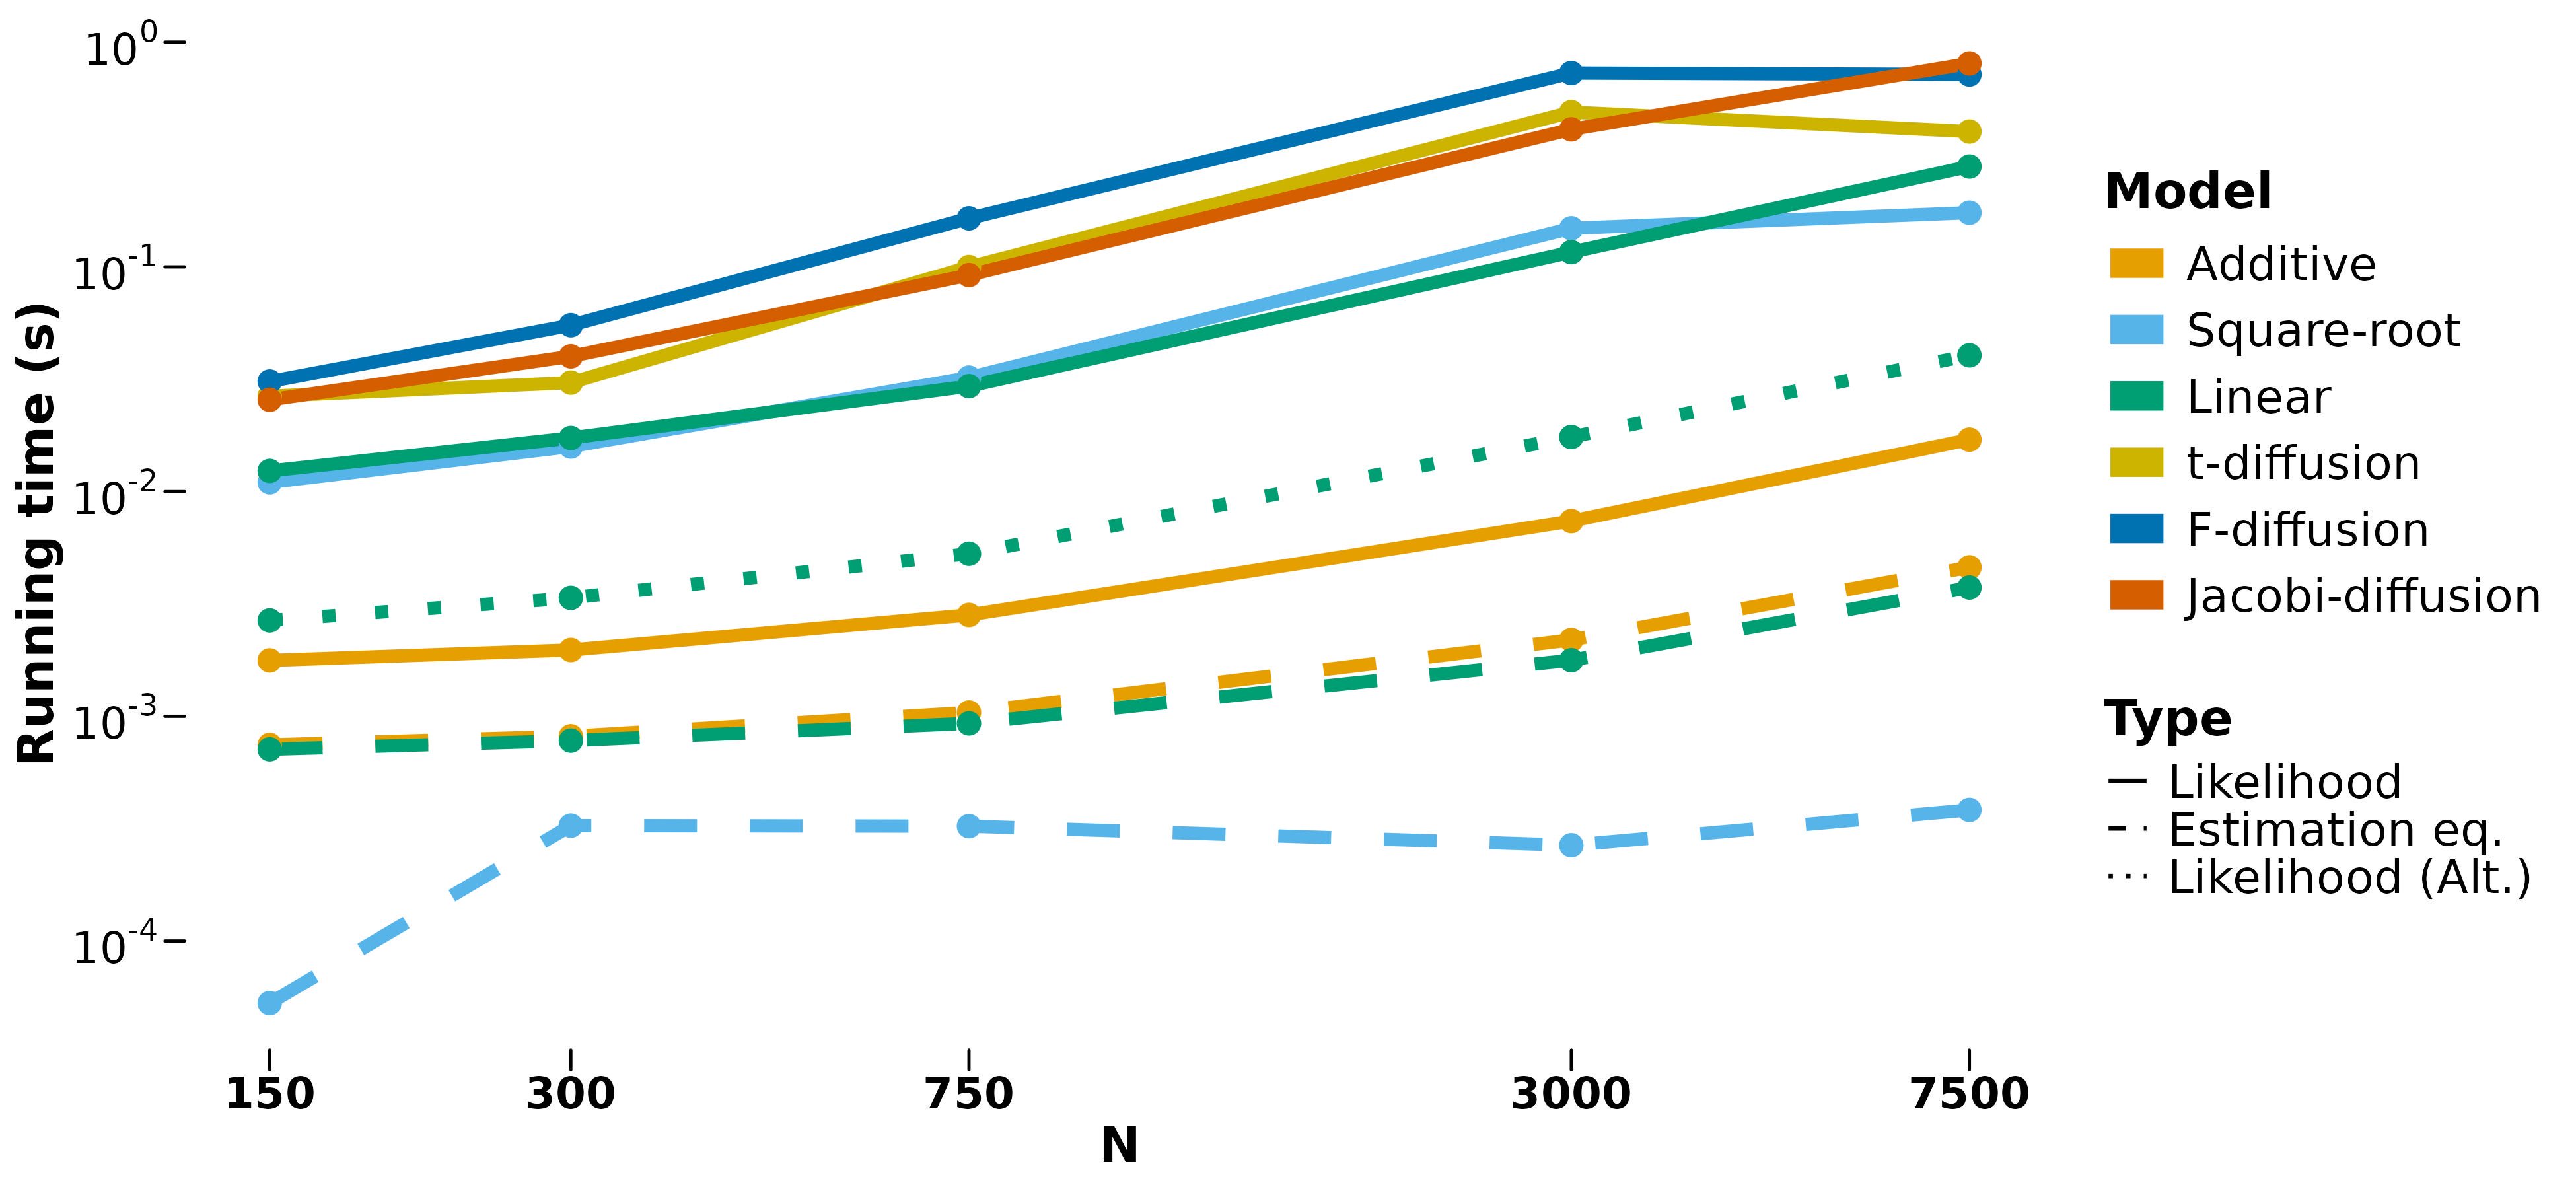
\includegraphics[scale = .1]{figures/estimation_duration_stationary.jpeg}
    \caption{Overview of the median computation time for each method as a function of the number of samples}
    \label{figure:overviewOfDurationStationary}
    \end{center}
\end{figure}\\
By median computation time we understand the time from the invocation of the optimizer till the convergence criterion is reached. Generally, the estimation equation-based estimators are much quicker than the likelihood-based, while the explicit estimators based on (\ref{eq:squarerootMartingaleEquation}) for the square-root diffusion are in a league of it owns being between 100 and 1000 times quicker than the likelihood based methods. The latter are generally in the same order of magnitude in terms of performance. Though, the $F$-, $t$- and Jacobi-diffusion based models are slower than the linear and square root-based models. This might be caused by more complicated ordinary differential equations in these models, which the Runge-Kutta needs to solve repeatedly; compare the expression in (\ref{eq:squarerootStationarySplit2}) and (\ref{eq:GBM_StrangNonLinearODE_split}) with (\ref{eq:StrangTDiffusion}), (\ref{eq:FscaledSplitting}) and (\ref{eq:jacobiODE}). If we look at the likelihood-based methods that solve the ordinary differential equations numerically and contrast their computation time with the ones that either use MLE or has a closed-form solution to the ODE (\ref{meanrevertingGBMSplit1}), it is clear that there is a computational cost to solving the ODE numerically. However, all methods are fast even for the highest amount of samples in the test, $N = 7500$, no single estimator broke the one second barrier in median.
\subsubsection{The Dynamic parts}
Turning to investigating the estimation in the dynamic part of each model, recall that we only use variations of the Strang method for this. If more than one is used, it is denoted \textit{Strang (Alt.)} here. The alternative Strang estimators are the ones that do not use the Lamperti transform, i.e. the two estimators based on (\ref{eq:squareRootSplit2}) and (\ref{eq:GBMSplit2}) used in the square root- and Linear models, respectively. We simulate from the models and fit the parameters in the manner described above. The ARE of the parameters in the dynamic part is depicted as a function of $N$ using a double logarithmic scale 
\begin{figure}[h!]
    \begin{center}
    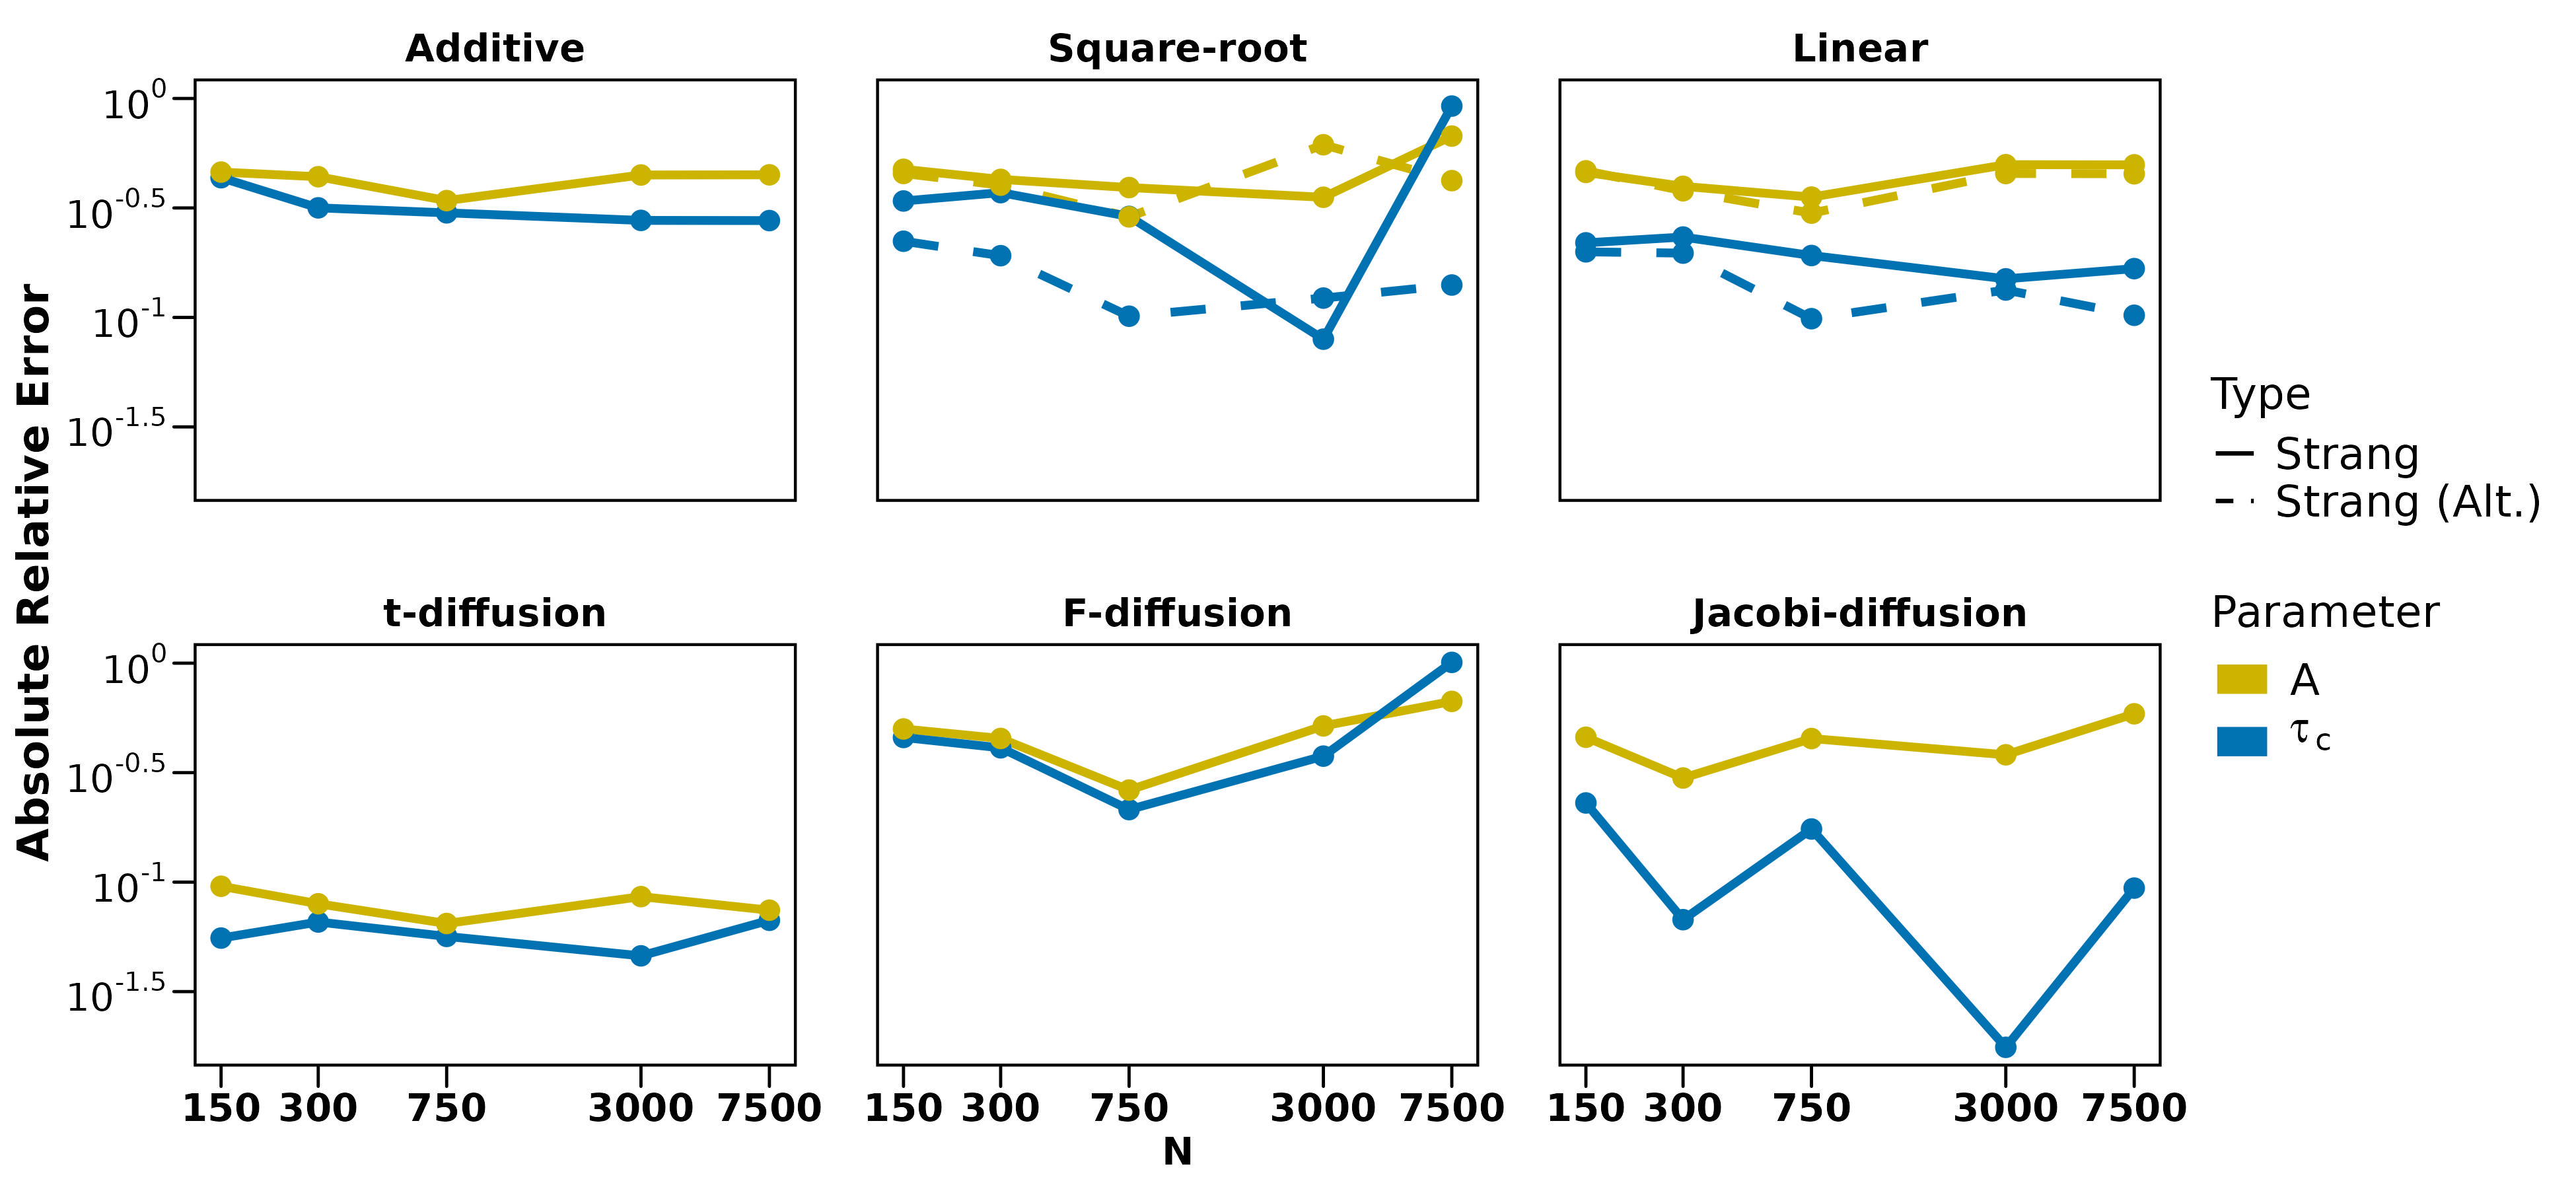
\includegraphics[scale = .1]{figures/parameter_precision_dynamic.jpeg}
    \caption{ARE of the parameters of the models in the dynamic part}
    \label{figure:parameter_precision_dynamic}        
\end{center}
\end{figure}\\
Due to the strong non-linear effects, it is generally harder to estimate in the dynamic part. In terms of the $A$-parameter all models and type of methods faired relatively equally in terms of ARE. That is with the exception of the $t$-diffusion model, whose ARE are around half an order of magnitude smaller than that of the other models. For some reason, the normal Strang-based estimator in the square root model as well as the $F$-diffusion-based model show a relatively high median ARE for the largest number of samples we investigated.  Considering the other sample sizes this is more surprising for the square root noise model, as it is generally easier to estimate in. The $F$-diffusion seems, on this scale at least, to be the hardest of the models to do estimation on; whereas, as we mentioned, the $t$-diffusion-based model seems to be the nicest. 

In terms of overall run time, we achieved similar results in terms of which kinds of models had faster convergence as we saw in Figure \ref{figure:overviewOfDurationStationary}. For this reason, the results are only shown in Appendix \ref{section:benchmark} in Figure \ref{figure:estimation_duration_dynamic}. One surprise from this benchmark though, is the fact that $t$-diffusion-based model, which solves its ODE numerically, has the fastest convergence of all the models. This probably stems from the model requiring fewer iterations overall before convergence is reached, as solving the ODE with Runge-kutta is much more computationally expensive than just computing the solution directly.
\subsection{Fitting the \texorpdfstring{$\nu$}{nu}-parameter}
We now consider how introducing the $\nu$-parameter into the model affects the performance of the optimizers. For simplicity, we focus on the additive- and t-diffusion-based models in this experiment. We ensure that the Brownian motions in a specific run in the simulation are the same. We simulate from both models using $t_0 = 54$ and $\tau_c = 132$ and temporal resolutions $\Delta t = \{1/3, 1/5, 1/25, 1/50, 1/100\}$, which correspond to $N_\mathrm{dynamic} = \{396, 660, 3300, 6600, 13200\}$ samples in the dynamic part. The dynamic part is the important one here because this is where $\nu$ is estimated. Of course, the quality of the estimates in the dynamic part hinges somewhat on the estimates from the stationary part.

The other parameters are $\theta = (A\; m\; \lambda_0\; \sigma)^\top = (0.87\; -1.51\; -3\;  0.387)^\top$. Due to its non-central role in this experiment, optimization in the stationary part is merely initialized in the true parameters, and the estimates are passed onto the optimizer in the dynamic part. In the dynamic part, optimization is initialized in a similar manner to earlier experiments. We add $\pm 10\%$ multiplicative noise to the true values of $A$ and $\tau$ by sampling two uniform variables according to $U\sim \mathrm{Unif}(0.9,1.1)$. The last parameter $\nu$ is always started in $1$, regardless of the true value. This is done to simulate the user assuming the more parsimonious with $\nu = 1$ and then letting the data show that $\nu$ is something else. 

For each value of $\Delta t$, we investigate how the models and optimizers perform on $\nu_{\mathrm{sim}} = \{0.75, 0.9, 1, 1.11, 1.33\}$. For each combination, we run $M = 50$ simulations. As earlier, we consider the median of the ARE for each combination of $\Delta t$ and $\nu$. The experiments are once more implemented such that failure to converge or run the optimization results in a graceful exit. Now, instead of merely retrying after a failed optimization attempt, we count how many times each model fails for every combination of $\Delta t$ and $\nu$. This is to highlight if there is a specific model or parameter value of $\nu$ that is troublesome to estimate in. The relative tolerance convergence criterion in \code{optim} was set to \code{sqrt(.Machine\$double.eps) / 1000} to avoid getting stuck in local minima. 
\newpage
\noindent We start by considering the ARE 
\begin{figure}[h!]
    \begin{center}
        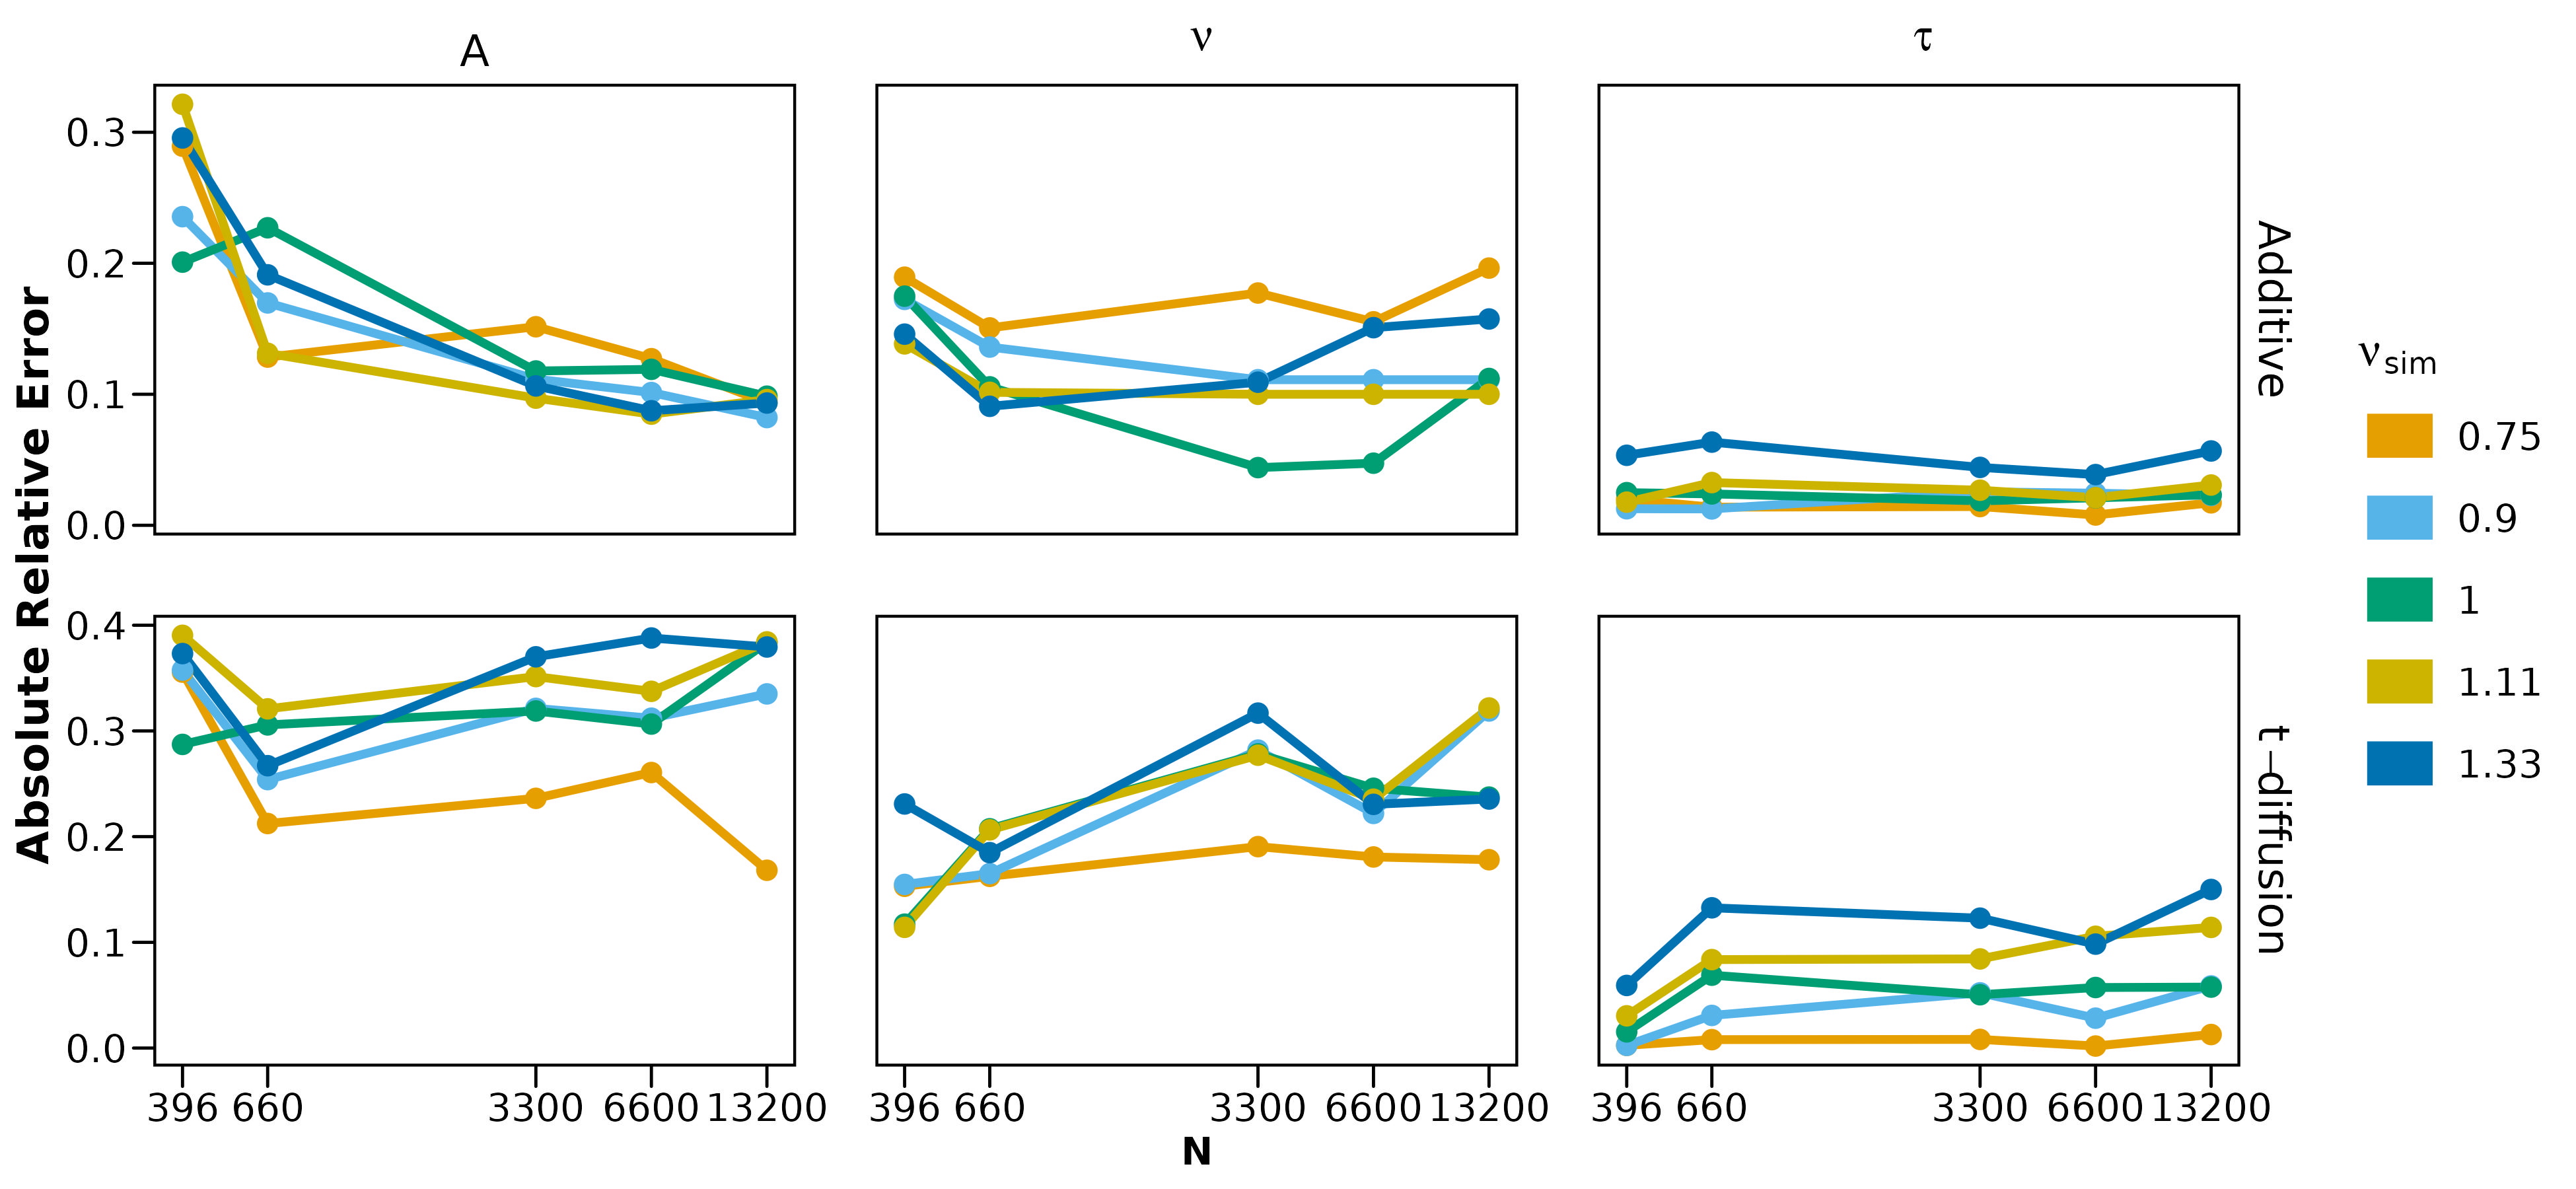
\includegraphics[scale = .1]{figures/combined_nus_plot.jpeg}
        \caption{The absolute relative error of the different parameters as a function of $N$ for diffferent true values of $\nu$.}
        \label{figure:ARE_nu_plots}
    \end{center}
\end{figure}\\
Note that the $x$-axis is logarithmic in Figure \ref{figure:ARE_nu_plots}. From the graph, we see that increasing the number of samples only really makes the median ARE better for the model with additive noise and only considerably for the $A$-parameter. However, the median ARE for the other parameters are generally low. Increasing the true value of the $\nu$-parameter does result in an overall larger ARE. If we look at Figure \ref{figure:nu_plot}, this is not too surprising. As we also commented on the graph, increasing $\nu$ results in the two fixed points being closer to one another longer before the bifurcation point. This creates a situation, where the process tips due to noise more frequently — thus making it difficult to estimate when bifurcation tipping would occur. All in all, though, the values depicted here do not seem too alarming considering the added flexibility having a $\nu$-parameter provides. 
\newpage 
\noindent However, they do not constitute the full picture themselves; we also counted how many times each method failed during optimization — yielding the following results
\begin{figure}[h!]
    \begin{center}
        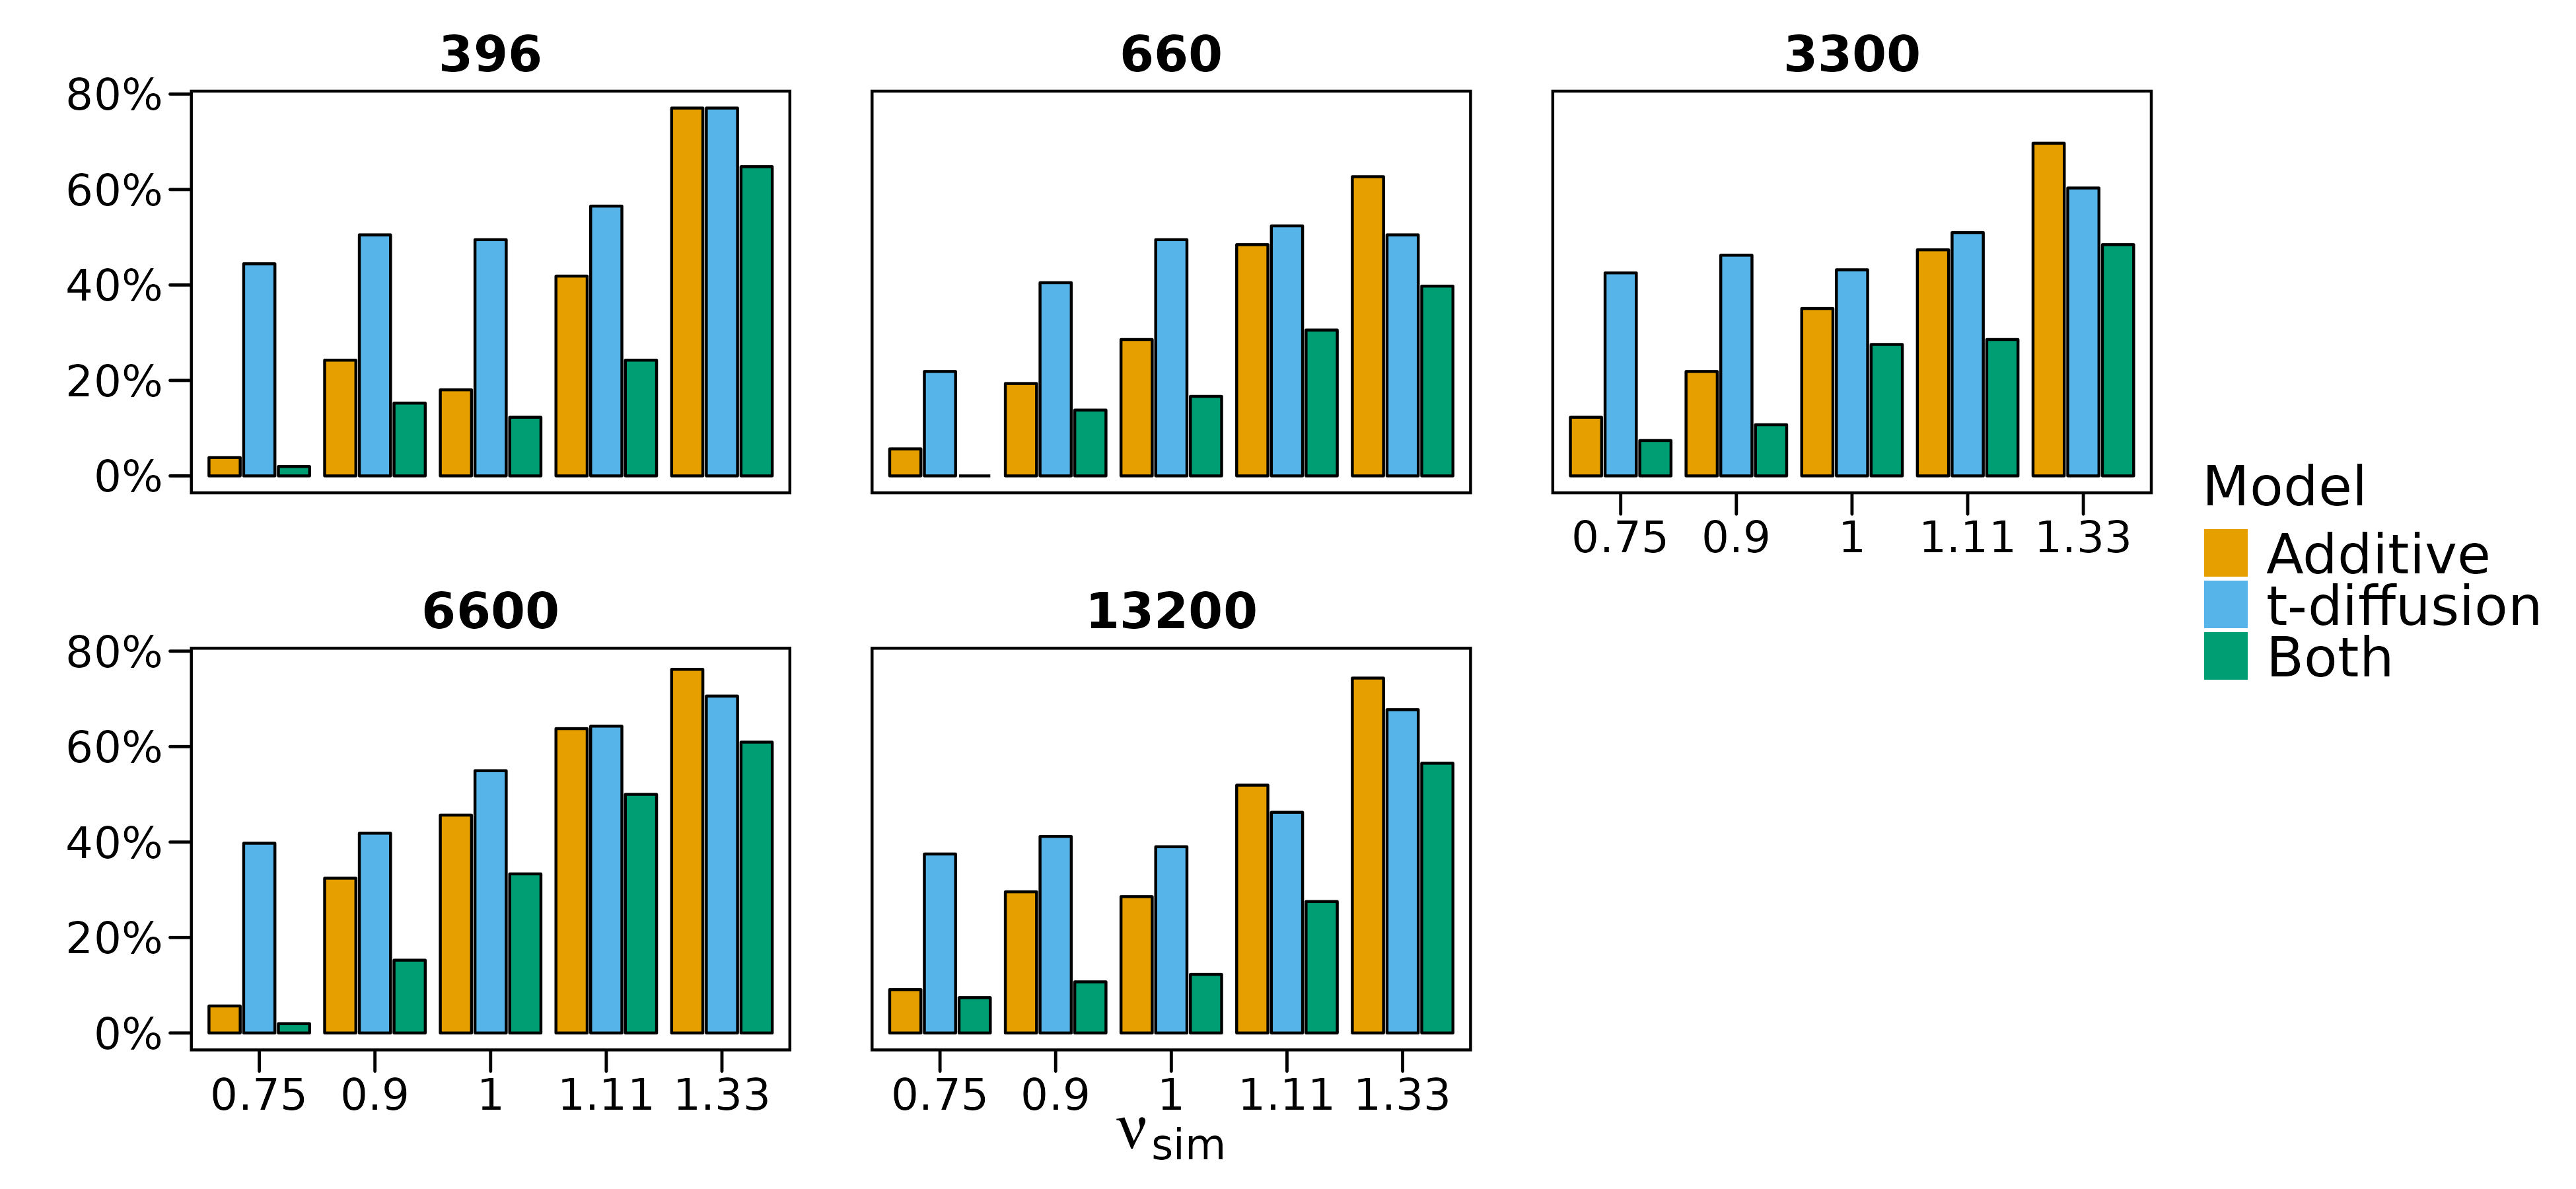
\includegraphics[scale = .1]{figures/error_count_plot.jpeg}
        \caption{The proportion of times where the respective models or both failed doing optimization as a function of $N$ and for different true values of $\nu$.}
        \label{figure:error_count_nu_experiment}
    \end{center}
\end{figure}\\
Keep in mind that the $x$-axis is now $\nu_{\mathrm{sim}}$, whereas the individual elements in the grid correspond to graphs for different values of $N$. Evidently, estimating with $\nu$ in the model estimation fails quite frequently. This is even when we a provided with estimates from the stationary part, where optimization was initialized in the true values. In comparison, we have virtually never during testing experienced the methods fail to optimize, when we only opt for estimation of $A$ and $\tau_c$ in the dynamic part. Now, the model with additive noise faires better overall and it seems that as long as the true value $\nu\leq 1$ the is a reasonable chance of success with it. However, this provides little consolation, as we do not know this in actual applications. Furthermore, we would, of course, like to be able to estimate in models with $\nu > 1$ too.\\\\
At the same time, the methods do not seem to improve for larger sample sizes, unfortunately. In addition, the $t$-diffusion-based model has for all sample sizes a $20\%$ chance of failing at best, which is unacceptable. From the green bar it is also rather clear that whenever the additive model do fail, it is often the case that the $t$-diffusion-based model fails as well, suggesting that the former is more stable, for this choice of parameters at least.
%\subsection{Early warning analysis}
\subsection{The Numerical Strang method}
We introduced the idea of the numerical Strang splitting in section \ref{subsection:NumericalStrangSplitting}. In sum, the aim was to numerically do as many of the computations to make a Strang splitting scheme that follows the heuristic in \cite{SplittingSchemes} as possible. The implementation we ended up with only needed to be provided the lamperti transform and the drift of the Lamperti-transformed SDE, and then it would take care finding fixed points, constructing the linear SDE etc. In this section, we contrast the numerical Strang applied to two models with their respective analytical counterparts. The ones we consider are the model with linear noise and the $F$-diffusion-based model. 
These models have their ODE solved numerically, meaning that the terms "analytical" and "numerical" should be understood relatively. For clarity, we will instead in the following refer to the "analytical" method as \textit{closed-form} alluding to the fact that it is the one where we use the closed-form solution of the fixed point For their Lamperti transform confer Table \ref{table:ergodicDiffusions}, while the Lamperti drifts can be found at (\ref{eq:GBM_lamperti}) and \ref{eq:F_diffusion_lamperti_SDE}. Because of the time dependence of the fixed points through $\lambda_t$ in the dynamic parts, we did not consider these, as it would be much more difficult to implement a method that finds a fixed point for each time point in a process. However, we later discuss how one could potentially overcome this obstacle.\\\\
We simulate using $A = 1.5$, $m=0.4$, $\lambda_0 = -0.2$ and $\sigma =0.15$ as well as $t_0 = 30$ with temporal resolution $\Delta t = \{1/5, 1/50, 1/150, 1/500, 1/1000\}$, which in other words means: $N =  \{150, 1500, 4500, 15000, 30000\}$.  The parameters correspond to $\alpha_0 = 1.095$, $\mu_0 = 0.7651$ and $\sigma = 0.15$ for the true parameters of the stationary part; these are the parameters we want to estimate. For each value of $N$, we run $M = 50$ simulations, do estimation and time the estimation with \code{microbenchmark}.

Optimization is initialized at noisy starting values as previously. This time the uniform variables are sampled such that each coordinate has a deviation from the true value of up to $\pm 25\%$ at random; though as before this noise is the same for all methods in a specific run of the simulation. As convergence criterion, we use the standard in \code{optim}: \code{sqrt(.Machine\$double.eps)}. We let the methods fail gracefully, but again keep track of how many times each method fails. Apart from this metric, we consider the distribution of the ARE to get a detailed view of how the methods perform — also in the extreme case. In this section, the results are shown for the model with linear noise as our findings are the most clear in this model. Still, the same results as we are about to show can be found for the $F$-diffusion-based model in Figure \ref{figure:ARE_dist_numeric_F_diffusion} in Appendix \ref{section:benchmark}. For the linear model, though
\begin{figure}[h!]
\begin{center}
    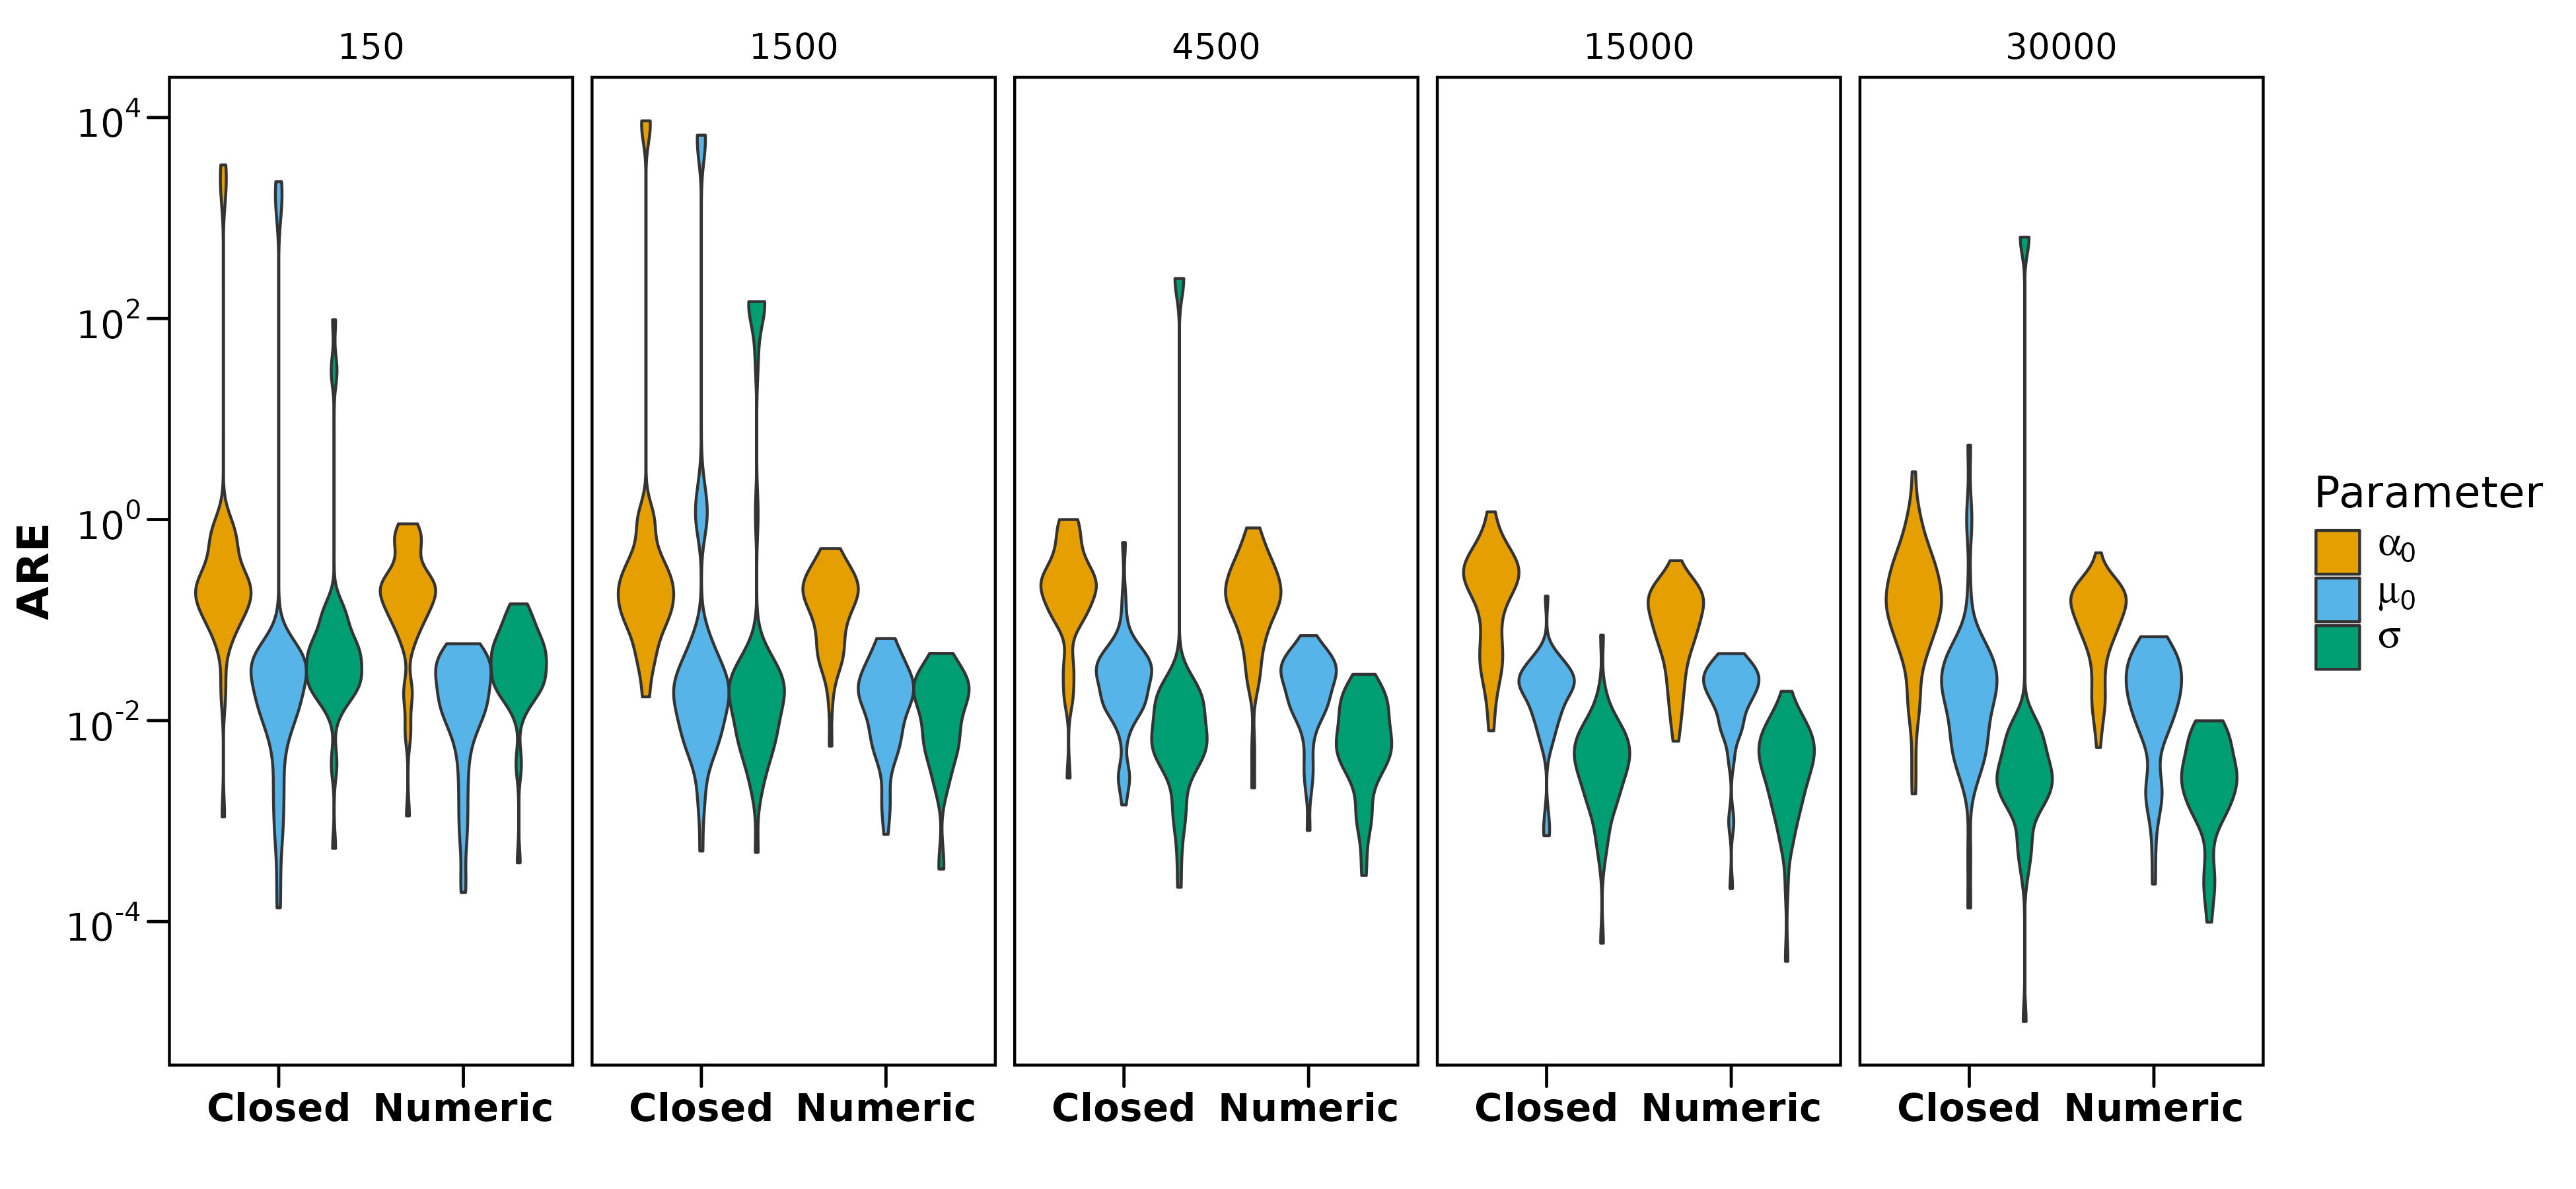
\includegraphics[scale = .1]{figures/ARE_dist_result_plot_Linear.jpeg}
    \caption{Distribution of the ARE of the parameters in the linear noise-based model shown for the numerical- and closed form type estimation methods.}
    \label{figure:ARE_dist_linear_noise}
\end{center}
\end{figure}\\
Initially, it is worth mentioning that across all runs in both models, it was only the closed-form solution of the linear model that ever failed to optimize. It did this around $20\%$ of the time for $N = 150$; $2\%$ for $N = 4500$ and $4\%$ for $N = 30000$, but never at other $N$. This fact aligns well with the results depicted in Figure \ref{figure:ARE_dist_linear_noise} as it suggests a lack of overall robustness of the method. In the graph, we see that there are a few quite extreme ARE-observations for parameters estimated by the closed form method. Conversely, a generally better performance of the numerical estimator is evident by the fact that the distribution of the ARE for a specific parameter and fixed number of samples is shifted towards zero for this estimator. 

Now, these results clearly speak for the numerical method. However, it is not difficult to come up with a potentially significant drawback of this method: Finding the fixed point, evaluating this point in the derivative of the drift via a finite difference-based method to then construct the ODE in the Strang splitting in a way where we cannot exploit any potential simplifications that might arise in the analytical expressions is bound to give us a method that is slower than the closed-form solution. Benchmarking the two methods for both models over the same runs that gave the results shown in Figure \ref{figure:ARE_dist_linear_noise} and - \ref{figure:ARE_dist_numeric_F_diffusion} yields the following run times:
\begin{figure}[h!]
    \begin{center}
    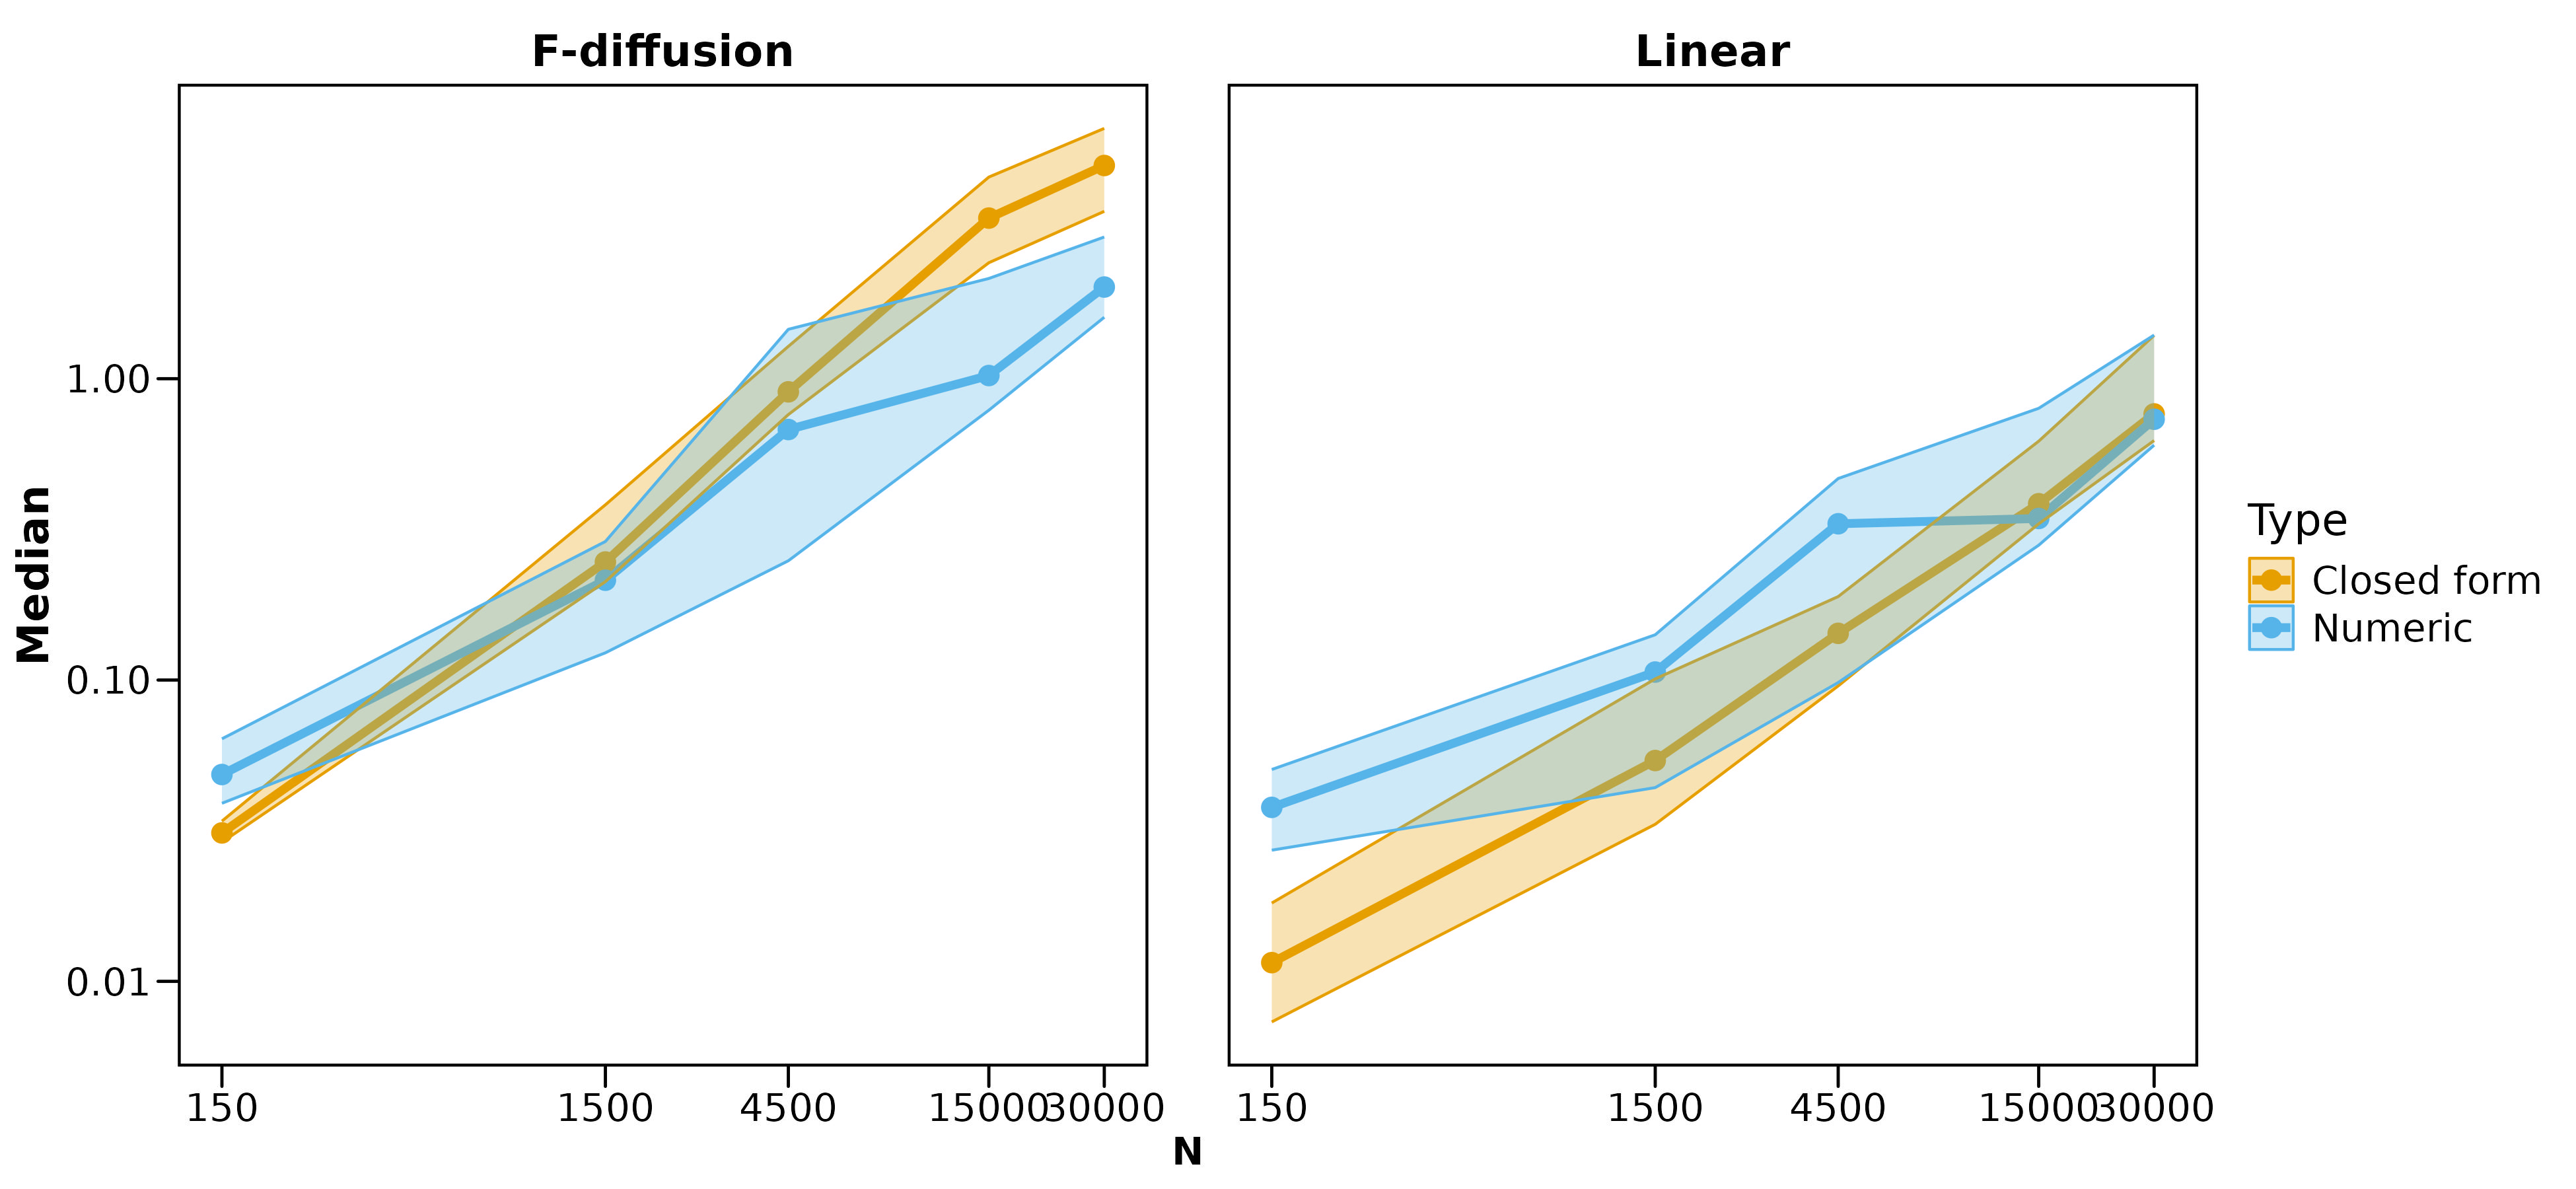
\includegraphics[scale = .09]{figures/Running_result_numeric.jpeg}
    \caption{Running times for the Linear-noise- and $F$-diffusion-based models stratified after type of Strang method.} 
    \label{figure:running_result_numeric}       
    \end{center}
\end{figure}\\
The borders of the shaded region constitute the $10\%$ and $90\%$ quantiles of the run times, while the solid line is the median run time. Also, note that Figure \ref{figure:running_result_numeric} is double logarithmic. Initially, we see what we might expect, the Numerical method has a relatively slow convergence in comparison to the closed form solution. However, for larger samples, this picture shifts completely for the $F$-diffusion, whereas the method is on par with the closed-form method in the Linear-noise model. This is a bit surprising as each call of the numerically-based objective function needs to do many more operations. Not only that but we also have to factor in the overhead of calling \code{nleqslv::nleqslv} and \code{numDeriv::grad} repeatedly. The added overhead might explain why the numerical methods are slower for smaller sample sizes as the overhead cost of a function call makes up more of the total run time in these instances. The effect of this added cost is negligible when the program spends more time doing actual computations. Still, the computations themselves should be slower even when we have more samples. \\\\
To see where the numerical method might gain its edge in terms of speed of convergence, though, we counted the number of times the methods had to evaluate the objective in order to find the minima. The \code{counts} output from \code{stats::optim} returns the number of evaluations of the gradient and function that was required for a specific run to convergence. Facetting over $N$, we depict this distribution for the Linear noise model grouped after what \textit{Type} of evaluation the objective used. We get the following distribution
\begin{figure}[h!]
    \begin{center}
    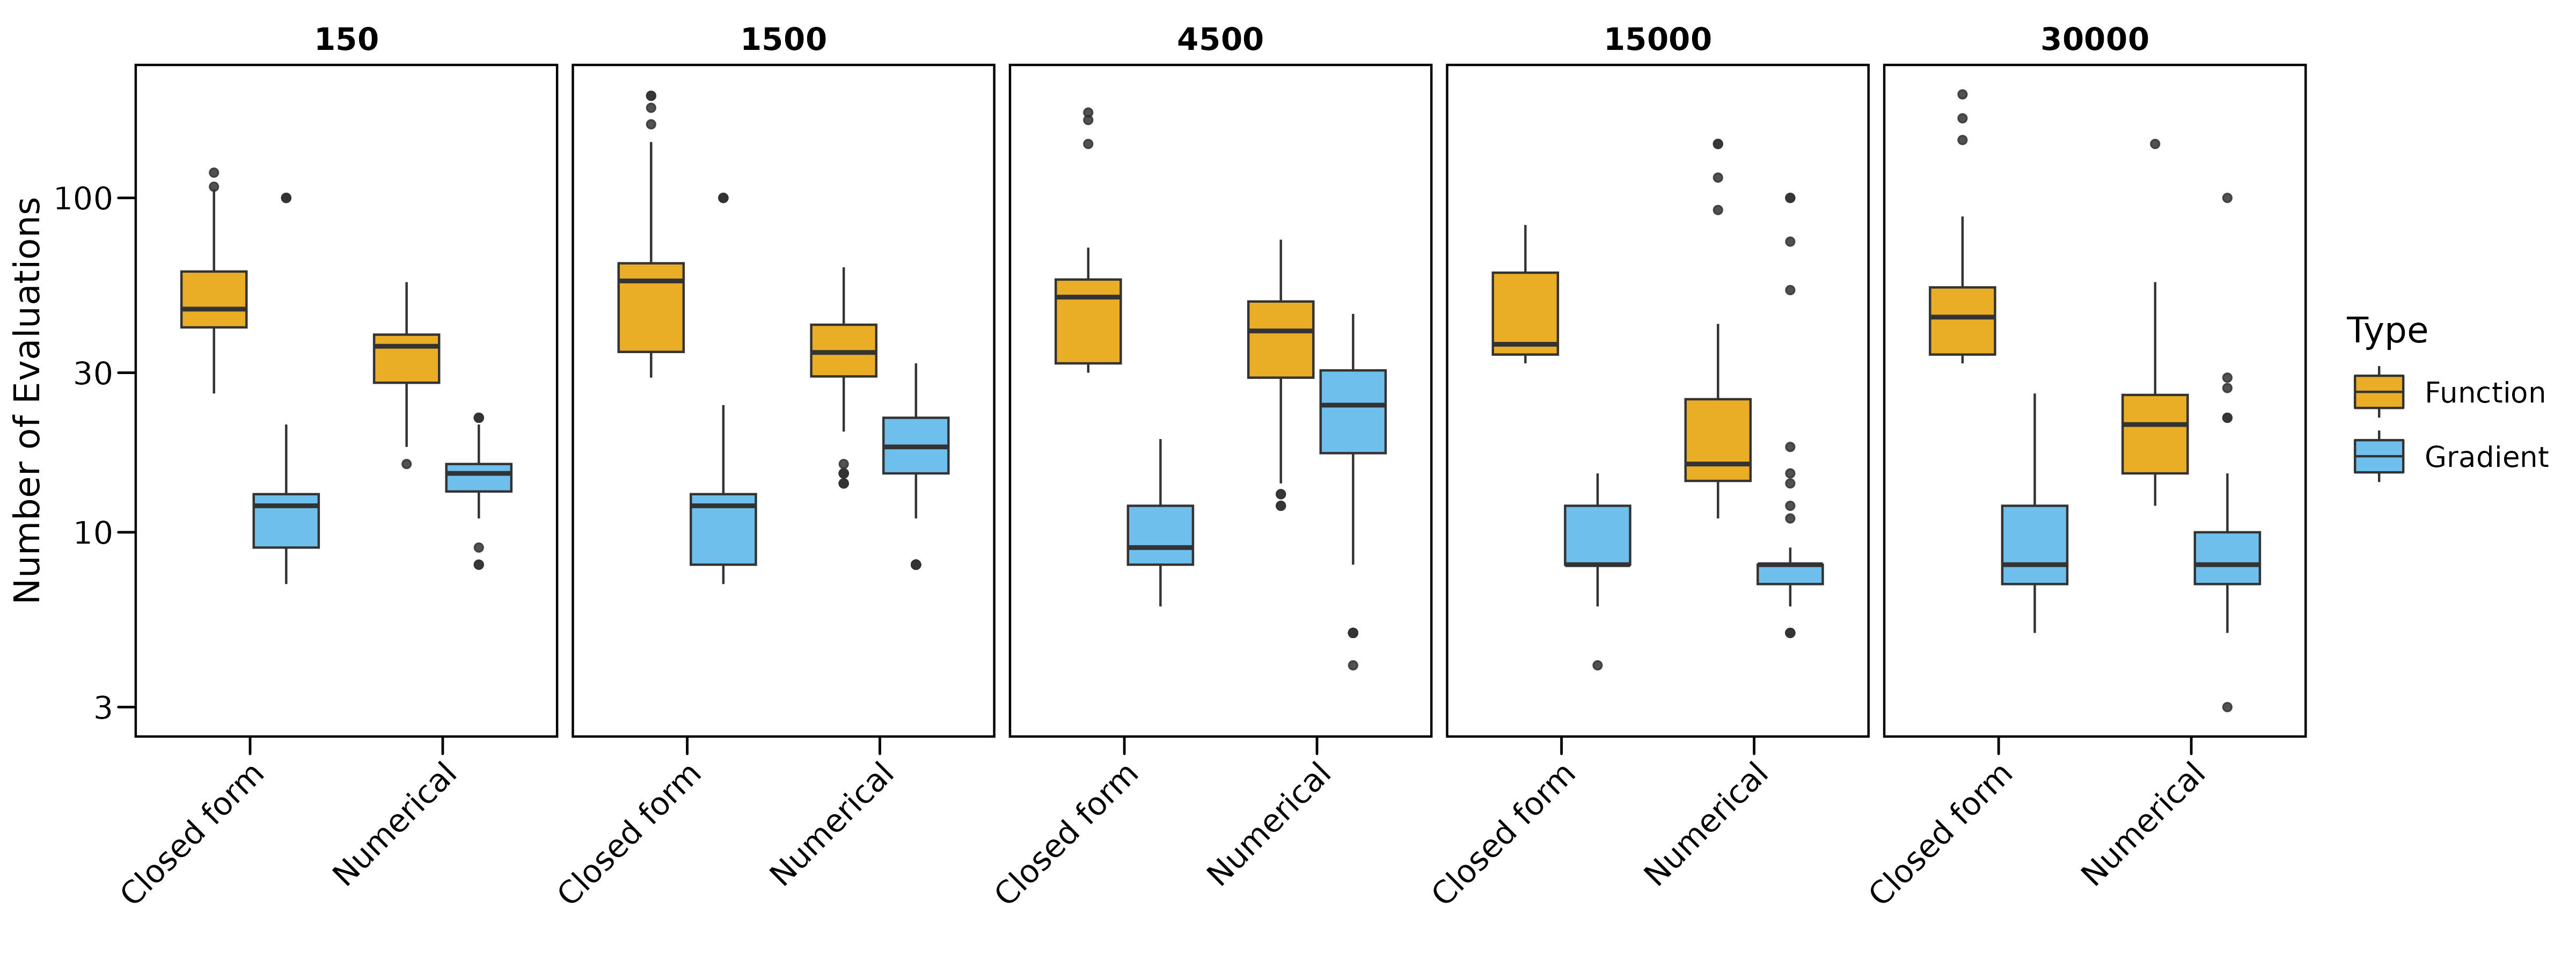
\includegraphics[scale = .08]{figures/function_gradient_count_Linear_plot.jpeg}     
    \caption{Number of gradient- and function evaluations for the two methods in the experiment on the Linear-noise model}
    \label{figure:linearFunctionGradientCount}   
    \end{center}
\end{figure}\\
Again note that to cater to the reading experience we have used a logarithmic scale on the $y$-axis. A similar plot for the $F$-diffusion-based model can be found in Appendix \ref{section:benchmark} in Figure \ref{figure:FFunctionGradientCount}; however there the difference between the methods is not as pronounced. In Figure \ref{figure:linearFunctionGradientCount}, though, we see that the amount of direct function evaluations is generally higher for the closed-form solution, whereas the number of gradient evaluations is a bit lower in the closed-form type Strang method. We suspect that the function evaluations are generally less computationally heavy because we do not supply the gradient and \code{stats::optim} thus needs to use finite-difference-based methods. Albeit we cannot confirm this as we did not find a way for \code{stats::optim} to return this information to us. Although the amount of function calls needed seems to decrease a bit for the numerical method, the shift we saw in Figure \ref{figure:running_result_numeric} might stem from the computation time of each call scaling better in $N$.

Of course, this example only illustrates the numerical Strang performs better on these specific values of the parameters $\alpha_0, \mu_0, \sigma$. Still, it highlights the fact that numerical methods sometimes can achieve on-par or even better performance than their closed-form counterparts. As to the specific reason for this, we let that be up for further research.
\subsection{Model Misspecification}
In our final simulation study, we consider how misspecification in a model can have an effect on our estimate. The way we will investigate this is simply by sampling from the additive model, fitting the data with the additive- and $t$-diffusion models and considering what effect on the estimates this has. We could, of course, consider all the parameters, however as $\tau_c$ typically is the parameter of interest, we focus on it. The setup of our simulations is the following: We sample using the parameters that were found on the AMOC-fingerprint data with the additive model in \cite[Figure 6]{Ditlevsen2023}, i.e. $A = 0.87, m = -1.51, \lambda_0 = -2.69, \sigma = \sqrt{0.3}$. We do this with temporal resolution of $\Delta t = 1/12$ and $t_0 =54$. We vary the true value of $\tau_c$ in the values $\tau_c = \{35, 60, 90, 132, 175, 200, 250\}$. On each of these values, we run $M = 200$ experiments, where we simulate from the additive model, fit the models in the stationary parts using \cite[equation (S4-S6)]{DitlevsenSupplementary} as starting values and in the dynamical parts initialize the optimizers at the true values with the usual uniform noise. Here the noise is constructed such that the initial values deviate $\pm 15\%$ from the true values.

Note that in the fitting of the $t$-diffusion model the whole idea is that we pretend we believe it is the data-generating distribution. As such we naturally transform the data with the Lamperti transform (see Table \ref{table:ergodicDiffusions}) during the fitting of that model. For both models in all runs, we compute their uniform residuals for both the stationary- and dynamic parts. We collect the values of the empirical quantiles of them and add to them the corresponding quantiles of the standard normal distribution for comparison.

To also be able to investigate which direction an estimation might be biased we look at the relative error in the following; this is merely (\ref{eq:ARE}) without the absolute value. Due to the presence of negative values we cannot log-transform this graph. To cater for the viewing experience, we remove all instances with a relative error above 1.5 in absolute value. For a quick overview of how what effect this had we tabularize the number of occurrences with absolute relative error above 1.5 stratified after model and true value of $\tau$. This information can be found in Appendix \ref{section:benchmark} in Table \ref{table:AREabove1.5tauSim}. We plot the distribution of the relative error for the remaining runs 
\begin{figure}[h!]
    \begin{center}
    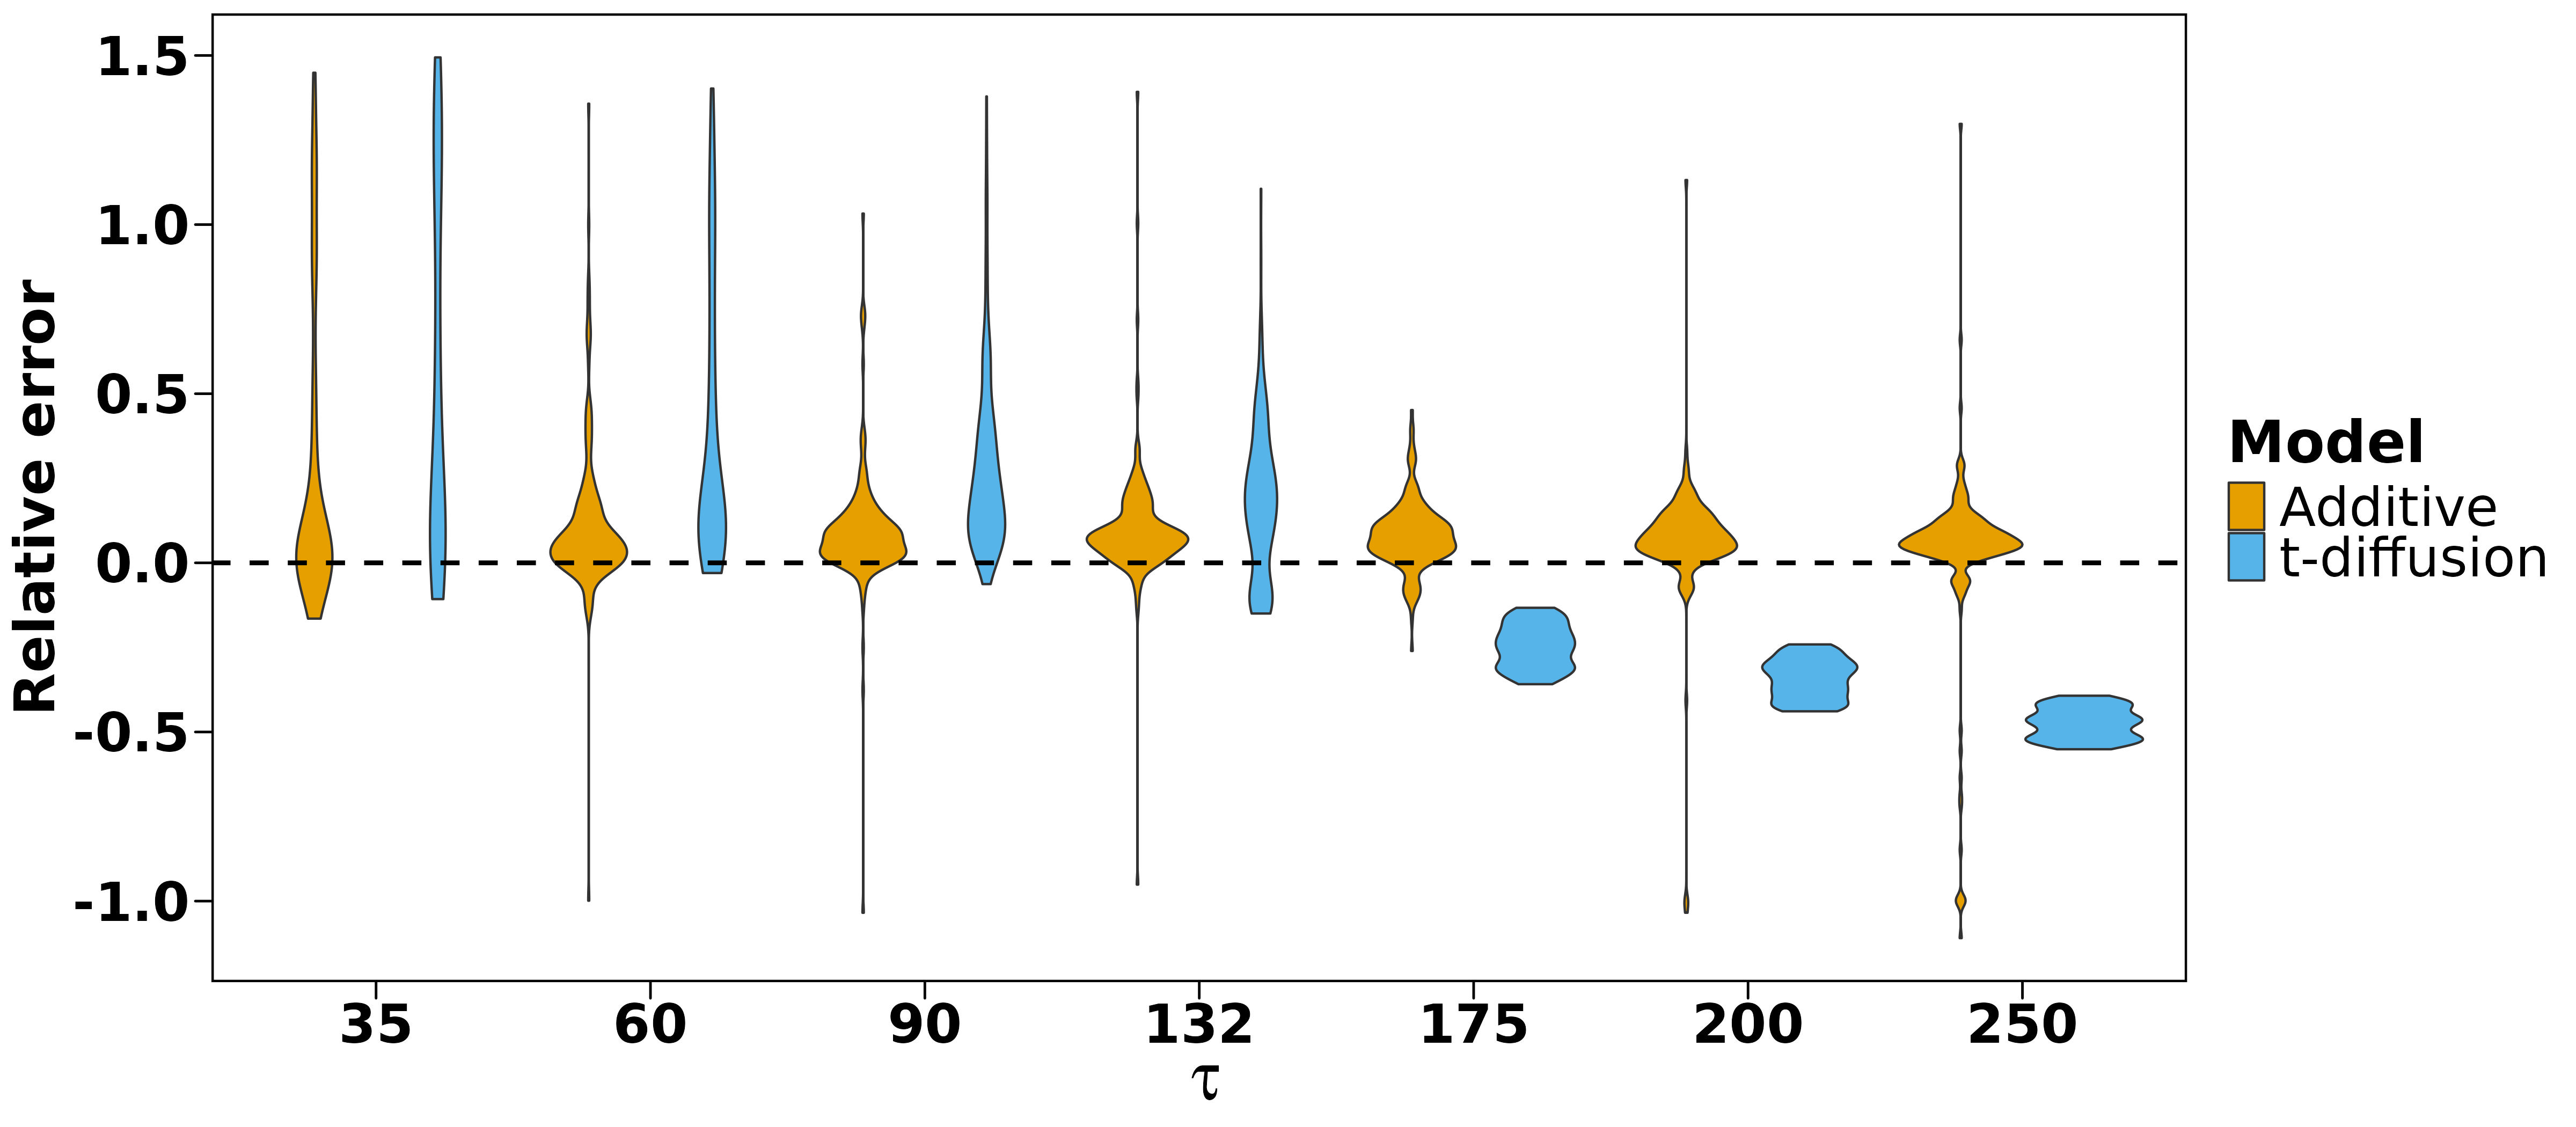
\includegraphics[scale = .075]{figures/RE_dist_tau.jpeg}
    \caption{Distribution of the relative error of the $\tau_c$-parameter stratified after the model it was fitted according to and size of the true value of $\tau_c$.}
    \label{figure:RE_dist_tau}
    \end{center}
\end{figure}\\
Interestingly, we see that the $t$-diffusion model actually estimates the tipping point alright as long as the true value is not too large. For $\tau_c = 35$ it is almost on par with the additive model. Though, generally it seems to overestimate the tipping point for smaller true values, while it underestimates it for larger true values of $\tau_c$. In addition, it seems that the additive model gets a bit biased for increasingly larger true values of $\tau_c$. The estimator based on this model seems to overestimate the tipping a bit, suggesting that for large $\tau_c$ it is inherently difficult to get the tipping point right with these methods.

However, the aim of this study is to mimic a real scenario a bit closer than this. In such scenarios, we do not have access to the true values of $\tau_c$ and we would instead need to consider the uniform residuals to diagnose the two models. In each run, we stored the range of quantiles as described above. Now, this gives $80.000$ observations in total of pairs of values for $q$ and its respective empirical $q$-quantiles from these simulations and depicting the empirical quantiles in a QQ-plot with the theoretical quantiles from the normal distribution is not very insightful.

Instead, we fit a linear normal model to the empirical quantiles stratified after whether it was the additive- or the $t$-diffusion-based model as well as the true value of $\tau_c$. If the models are properly specified the uniform residuals should generally lie on the identity, and the linear regression models should reflect this
\begin{figure}[h!]
    \begin{center}
        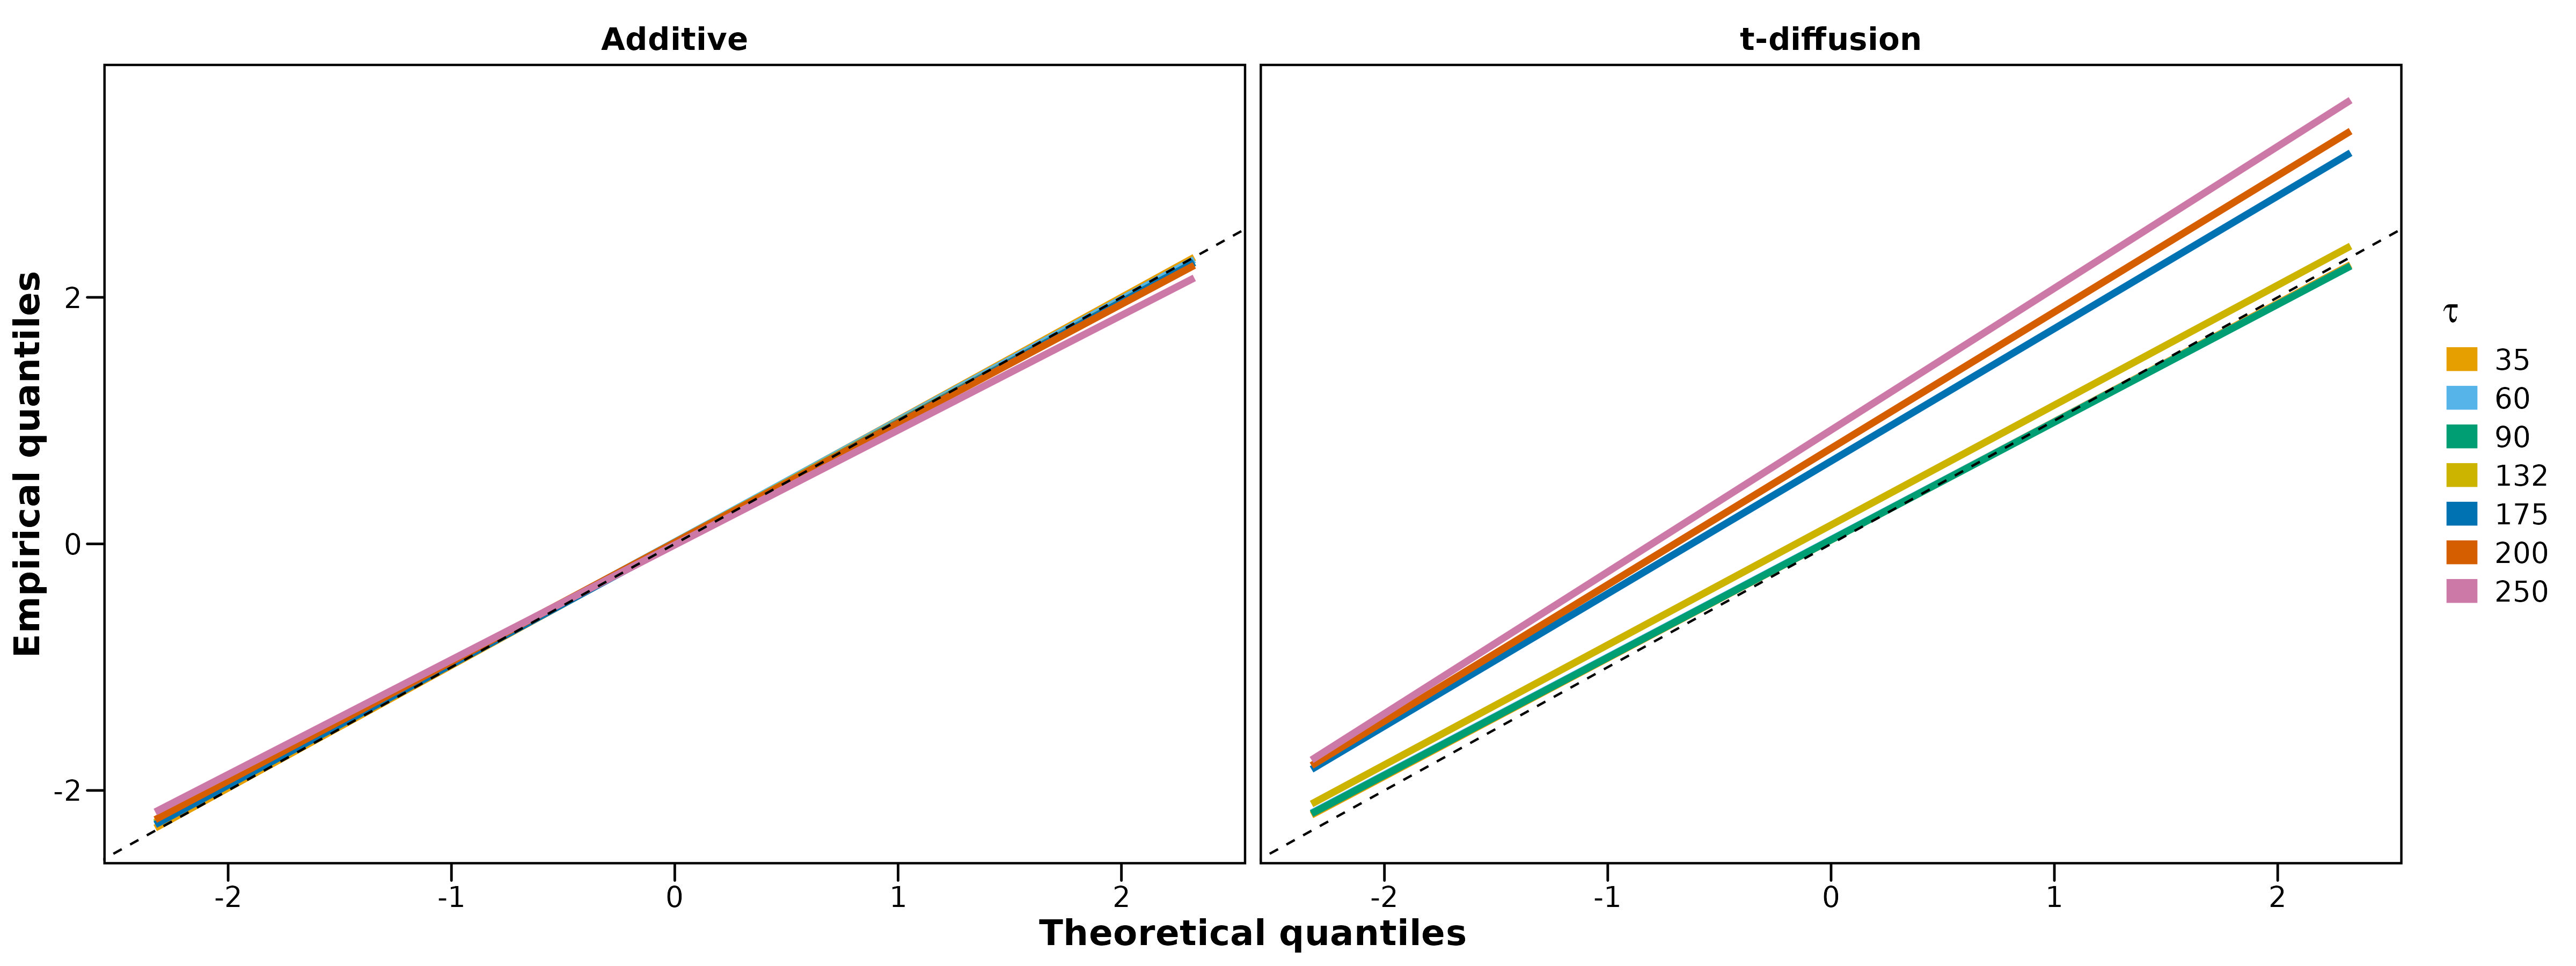
\includegraphics[scale = .075]{figures/quantiles_plot_tau.jpeg}
        \caption{Fitted linear models to data of pairs of theoretical- and empirical quantiles stratified after the true value of $\tau_c$ and the model used to fit the data.}
        \label{figure:QQ_plot_tau}
    \end{center}
\end{figure}\\
Note that the fitted lines in the $t$-diffusion facet for the true values of $\tau_c = \{35, 60, 90\}$ are almost atop one another, whence they are hard to distinguish in the graph. \\
The general impression across all runs is, luckily, that it is clear from the uniform residuals that the $t$-diffusion is misspecified. However, the fit seems alright for the true values for which we also noted from Figure \ref{figure:RE_dist_tau} it estimated $\tau_c$ relatively well. 
\section{Results}\label{Results}
We apply the estimation methods to proxies of two seperate systems: The Atlantic meridional overturning circulation (AMOC), where these methods were initially used \cite{Ditlevsen2023} and global climate variations.
\subsection{Tipping of the Atlantic meridional overturning circulation}
For the AMOC the time series we consider is the sea surface temperature (SST) anomaly in the subpolar gyre in the north Atlantic ocean in comparison to the the global mean SST anomaly. The SG SST minus twice GM SST has been argued to be a proxy of the strengh of the AMOC; twice is used in compensation for the amplificaiton of global warming in the polar regions \cite[caption of figure 1]{Ditlevsen2023}.
\begin{figure}[h!]
    \begin{center}
    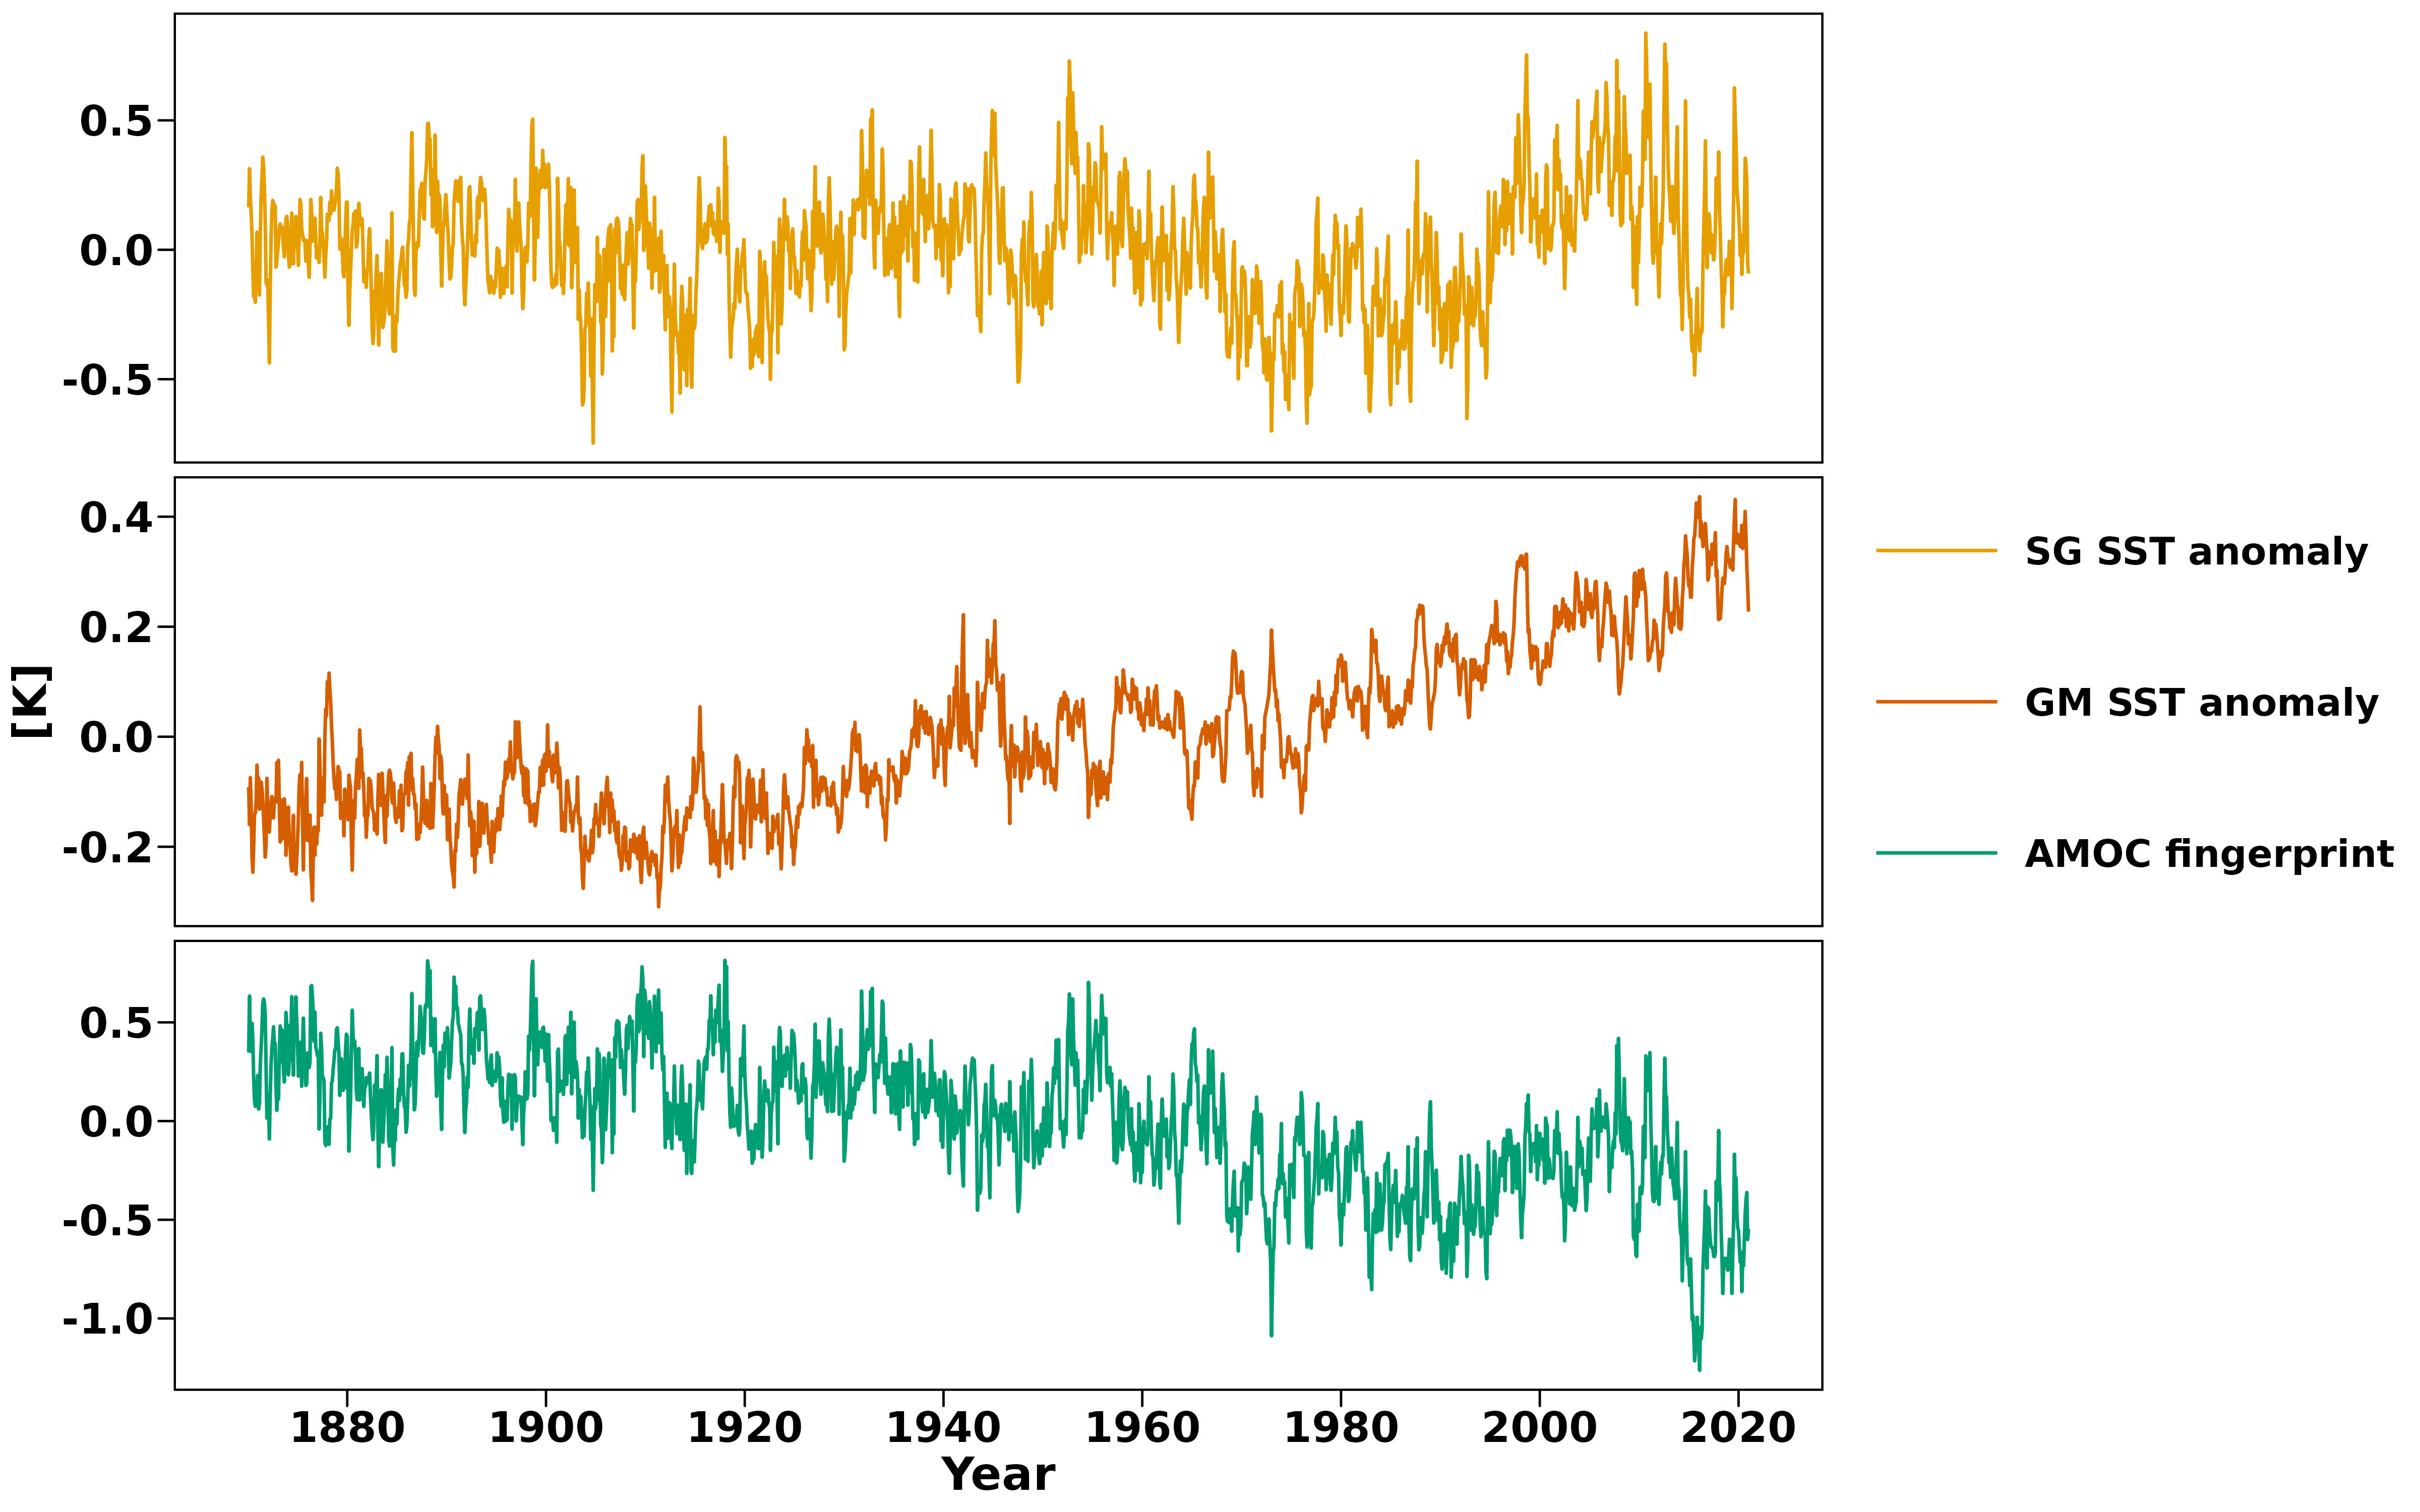
\includegraphics[scale = .075]{figures/AMOC_data_plot.jpeg}
    \caption{SST anomalies in the subpolar gyre and global mean as well as the AMOC fingerprint}
    \label{figure:AMOC_plot}
    \end{center}
\end{figure}
\subsection{Tipping in global climate variations}
Climate physicists have extensively studied ice core data from Greenland as the Greenland ice sheet acts as a sediment for the atmosphere. It is widely accepted that the ratio between the isotopes $^{18}\mathrm{O}$ and $^{16}\mathrm{O}$ is an indicator of the temperature at the time of accumulation. Additionally, $\mathrm{Ca}^{2+}$-ions from dust settle in the ice layer by layer. Unlike the ratio they do not diffuse as much; this allows us to have a finer temporal resolution. We can use calcium-ions instead of the ratio, because there is a negative correlation betwen the logarithm of the log-concetration of the $\mathrm{Ca}^{2+}$-ions and the isotope-ratio. This means that higher calcium-ion concentrations indicate colder global conditions. The ice-core data consists of observations of the oxygen isotope ratio and $\mathrm{Ca}^{2+}$-ion concentrations from $107620$ years before present to $10260$ years before present with a constant temporal resolution of $20$ years. We rescale to kilo years and focus on the observation of the calcium-ion between $86$ kilo years before present (kyrs bp) and $55$ kyrs bp; of course still with $\Delta t = 0.02$. Now, transforming ion-concentrations by $-\log (x)$ is a common practice in chemistry, whence we also consider $-\log([\mathrm{Ca}^{2+}]) - C$, where $C$ is a constant that makes the process have mean zero. We depict the ion-concetration over time
\begin{figure}[h!]
    \begin{center}
    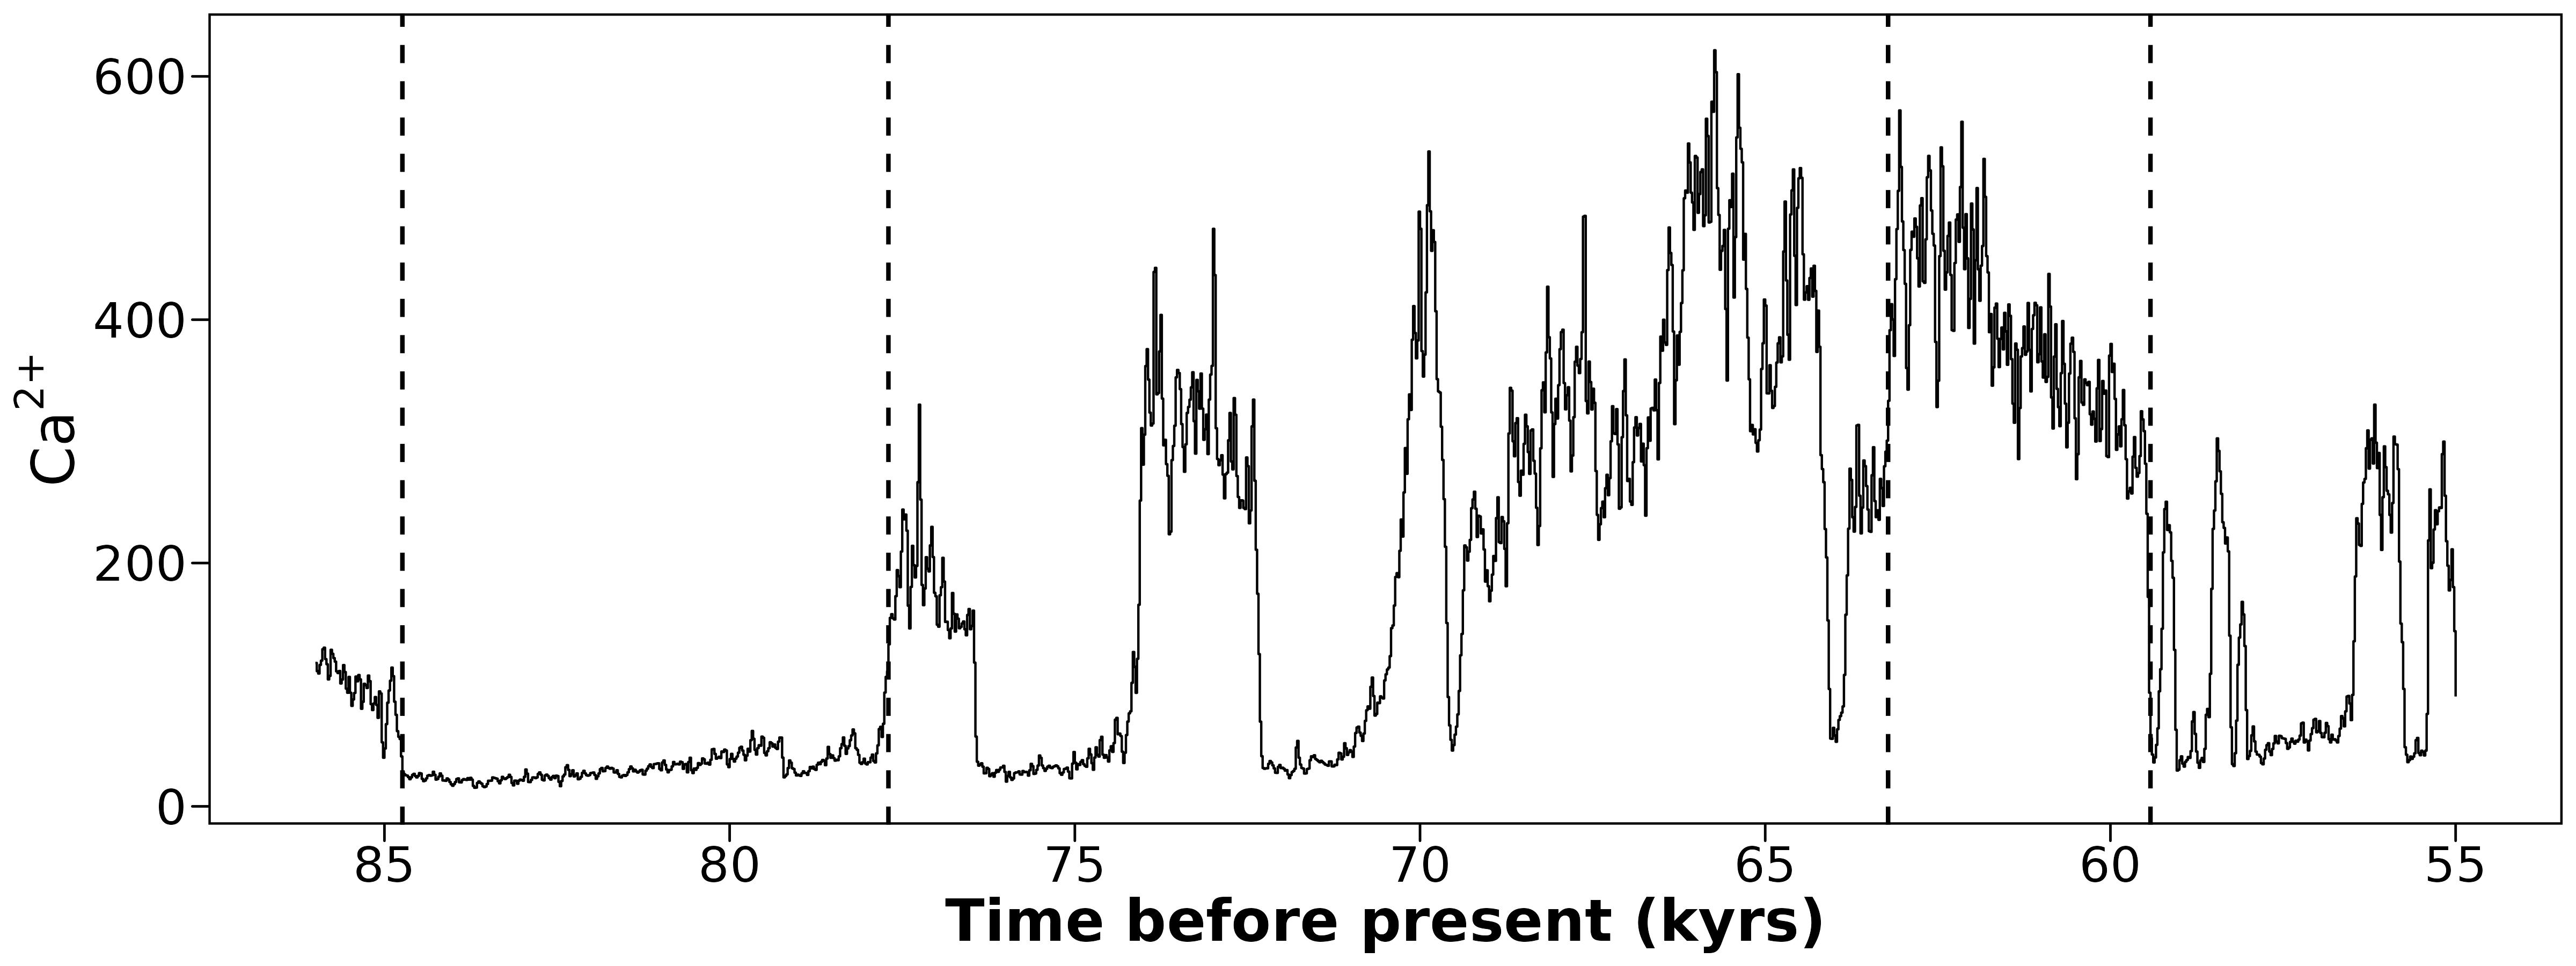
\includegraphics[scale = .075]{figures/ice_core_plot.jpeg}
    \caption{$\mathrm{Ca}^{2+}$-concetration in the ice sheet in the periode 86 kyrs bp to 55 kyrs bp}
    \label{figure:Ca_icesheet}
    \end{center}
\end{figure}\\
Looking at graph there are some periods of time where the concetration seem to be in somewhat of a stationary state. We have marked two periods that highlights to such periods by four vertical lines. The two periods we consider concentrations for are $[77.7, 84.74]$ and $[59.42, 63.22]$; these consist of 353 and 191 observations respectively. At the end of the two periods there seem to be a tipping to another state; to make this clear we zoom in on the time periods - note that we add some of the observations after tipping for illustrative purposes
\begin{figure}[h!]
    \begin{center}
    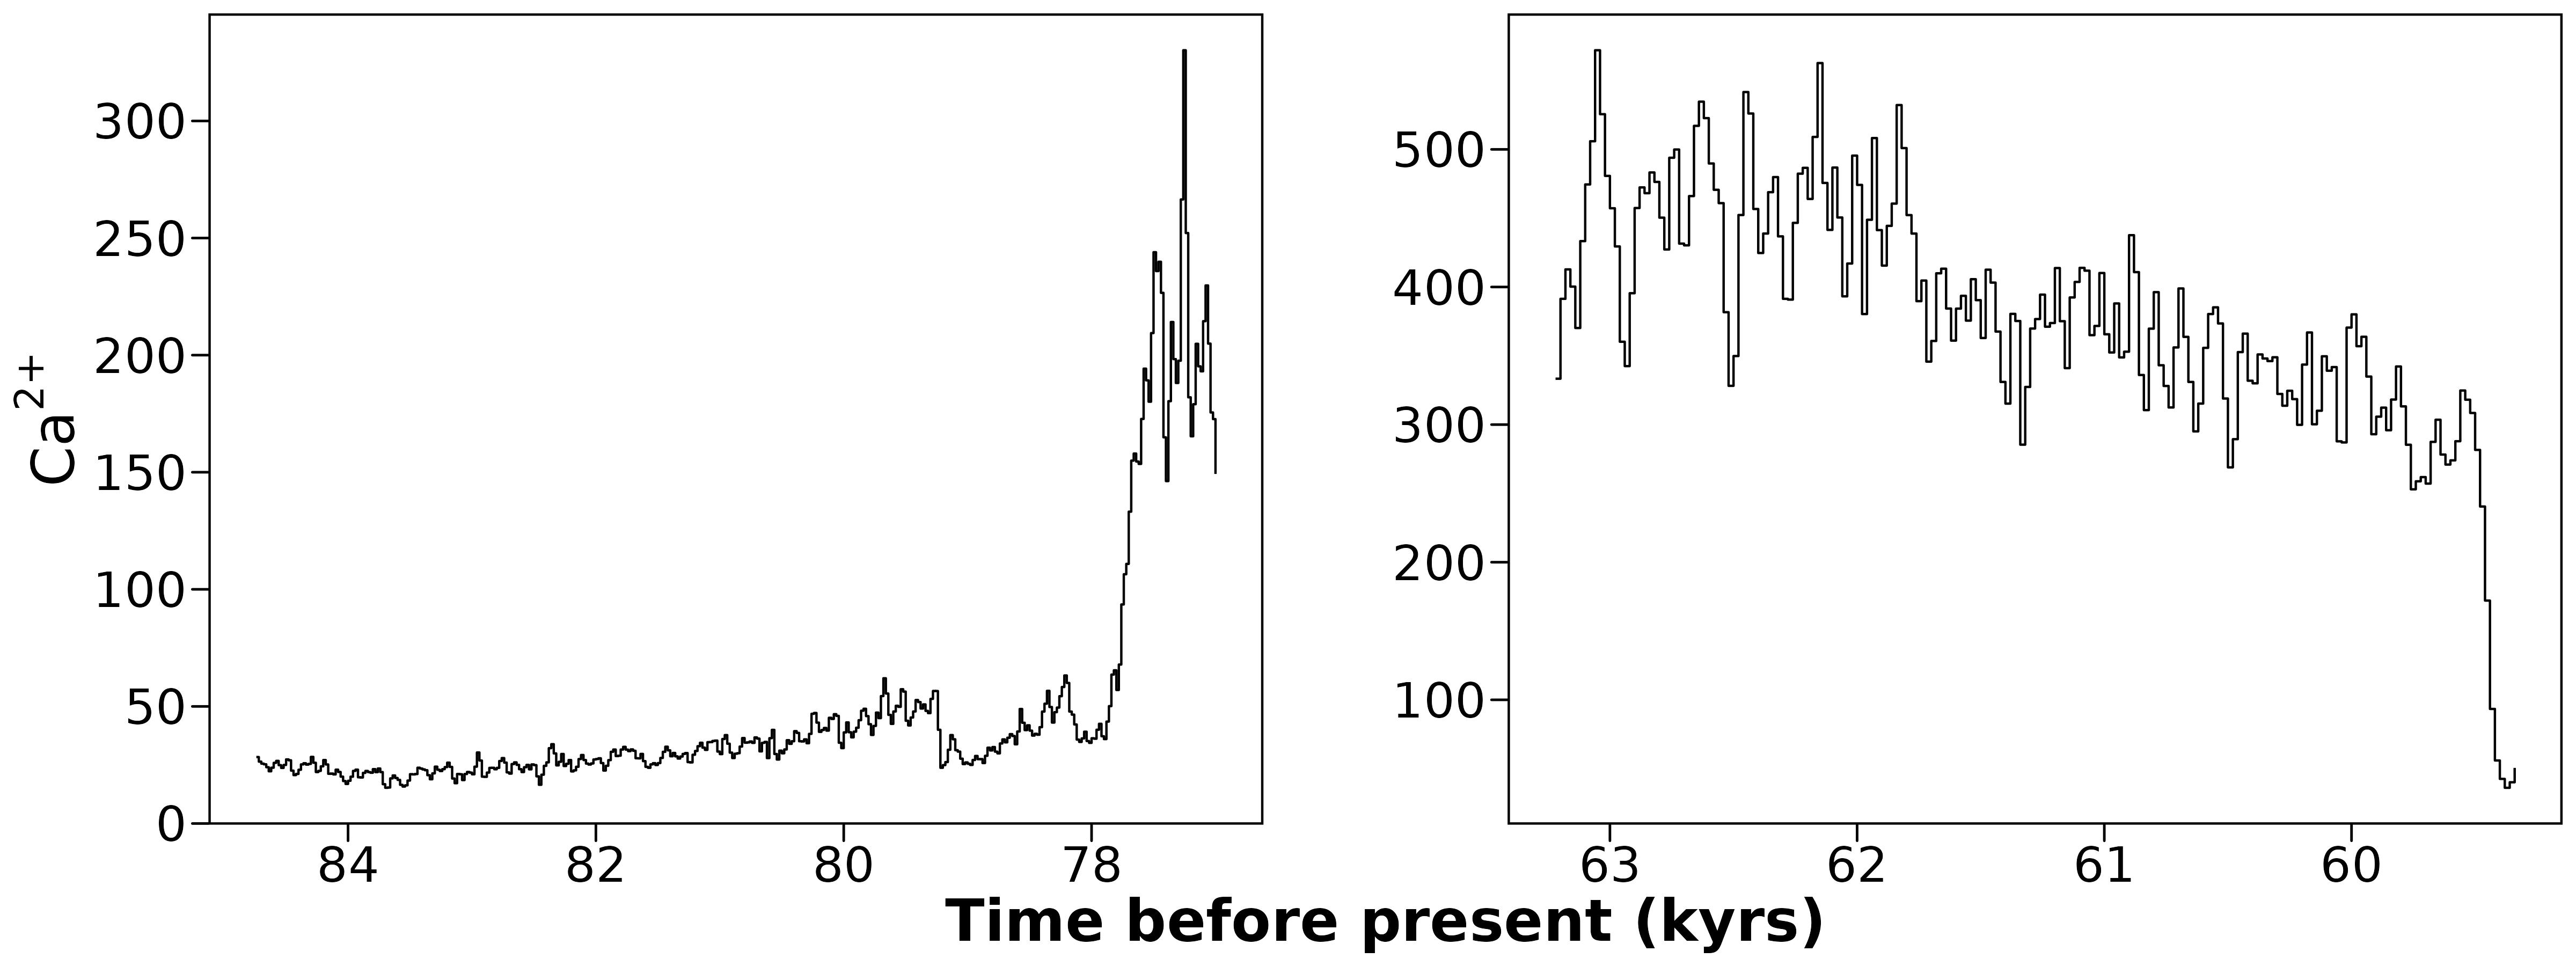
\includegraphics[scale = .075]{figures/ice_core_zoom_plot.jpeg}
    \caption{Zoom in on the $\mathrm{Ca}^{2+}$-concetration in the ice sheet in the two intervals of interest}
    \label{figure:Ca_icesheet}
    \end{center}
\end{figure}\\
We analyze both these periods using the mean-reverting geometric brownian motion based model.
\section{Discussion}\label{Discussion}
This discussion is structured into two semi-independent parts: We first summarize the results from the simulation study and reflect on how we can develop on the methods, especially on the numerical optimization side of things. Furthermore, we mention two estimation methods that could be interesting to consider in future research.

Then we put the results from the estimation of the AMOC into perspective, contrasting it with previous findings. Here, we also discuss how one might go about selecting between models from \ref{table:ergodicDiffusions}. In particular, with our models as a starting point, we discuss what type of role the stochastic part in these types of analysis can have. Additionally, we mention a couple of other ideas that can be used on these models in practice. In extension, we reflect on how one can think about these models in general.
\subsection{Simulation Studies}
Our starting point for the discussion is a short look into the results shown in Figures \ref{figure:parameter_precision_dynamic} and \ref{figure:overviewOfEstimatorsStationary}. As we noted, it is not given that the behaviour shown in these graphs is representative on all scales. Additionally, the experiment only tweaked the number of samples through the temporal resolution. In a future study, it would be interesting to investigate how longer (or shorter) time series affect the estimators in an otherwise similar experiment. With our simulation schemes, we can achieve this by changing the $t_0$- and $\tau_c$ parameters.

Another natural extension is to look into other evaluation metrics. We mostly considered the ARE and the computation time. One other metric we could have used more is the relative error. Another popular choice is just the difference between the estimate and the true value because it, with proper normalization, can be used to examine the distribution of the estimators more precisely. Although we have not stated them, many of our estimators have asymptotic results, which in principle can be demonstrated in these kinds of studies.\\\\
Other than that, we could consider changing the BFGS algorithm to other algorithms and study what effect tweaking potential hyperparameters for these might have. In continuation, specifying the gradients for the various methods might reduce the number of steps required for convergence at the minimum. Having a closed-form of the gradient likely makes evaluating it less computationally heavy than our current implementation as \code{stats::optim} uses finite-difference-based methods, when no gradient is provided. Albeit, currently the Ornstein Uhlenbeck is the only process for which we have implementations of both the likelihood and the score. However, to motivate further research, we conducted a small experiment that shows that the optimization can gain significantly from our providing a gradient to it. The result is shown in table \ref{table:smallOUExperiment}. To be able to apply the strategy outside of this case hinges on the Strang-based score being tractable. But if it were, we could use it in unison with the likelihood in the optimization. We also briefly considered using the martingale estimation equations from the mean-reverting GBM in unison with its Strang-based pseudo-likelihood. This was a bit more troublesome to get to work and the results were not as convincing, so we do not illustrate them here.  \\\\
Moving on, there is no doubt that at our current state of implementation, it is not feasible to estimate with a varying $\nu$-parameter in the models. As seen in Figure \ref{figure:error_count_nu_experiment} the optimization process is simply not robust enough to even try estimation on real data. It is probable that the challenges we have experienced stem from the fact that $\nu$ enters into the likelihood in quite a complex manner. By looking at Figure \ref{figure:nu_plot}, we see that the $\nu$-parameter shapes the overall evolution of the fixed point. What the plot also reveals is that relatively small changes around $\nu = 1$ result in quite different shapes, making estimation difficult.
 
Without any prior knowledge, the idea of starting optimization at $\nu = 1$ seems like the only fair way to do so. So before we find any reasons to deviate from this we stick with this strategy. However, this can obviously leave the optimizer with a difficult optimization problem, if this a poor initial value for optimizer. To remedy the issue of stability, one option we could try is to penalize values of $\nu$ relatively far away from $1$. Due to the form of (\ref{eq:lambdaRampDefinition}) straying relatively far away from $\nu = 1$ results in progressively smaller changes in the shape. In Figure \ref{figure:nu_plot} this can be seen by the shape of the fixed points not being as different for $\nu = 2.27$ and $\nu = 4.48$ as for instance $\nu = 1$ and $\nu = 1.65$. Therefore penalizing values much larger than $1$ and relatively close to $0$ might be a good choice to push the optimization away from these parts of the parameter space. In continuation of our discussion about providing gradients to the optimizer, the issue at hand might be another use case of this as lack of robustness might stem from the finite-difference-based methods used by \code{stats::optim}. \\\\
If we achieve more robust optimization with $\nu$ another consideration to make is to question when there even is enough information in the time series to estimate $\nu$ reliably. We would have liked to investigate this with a simulation study. Unfortunately due to the aforementioned issues, we can only illustrate this point intuitively here. To do so, we sample from the additive-noise model using the same parameters as in Figure \ref{figure:nu_plot}. The $\sigma$-parameter is set to $0.3$ and we sample with temporal resolution $\Delta t = 1/24$.
\begin{figure}[h!]
    \begin{center}
    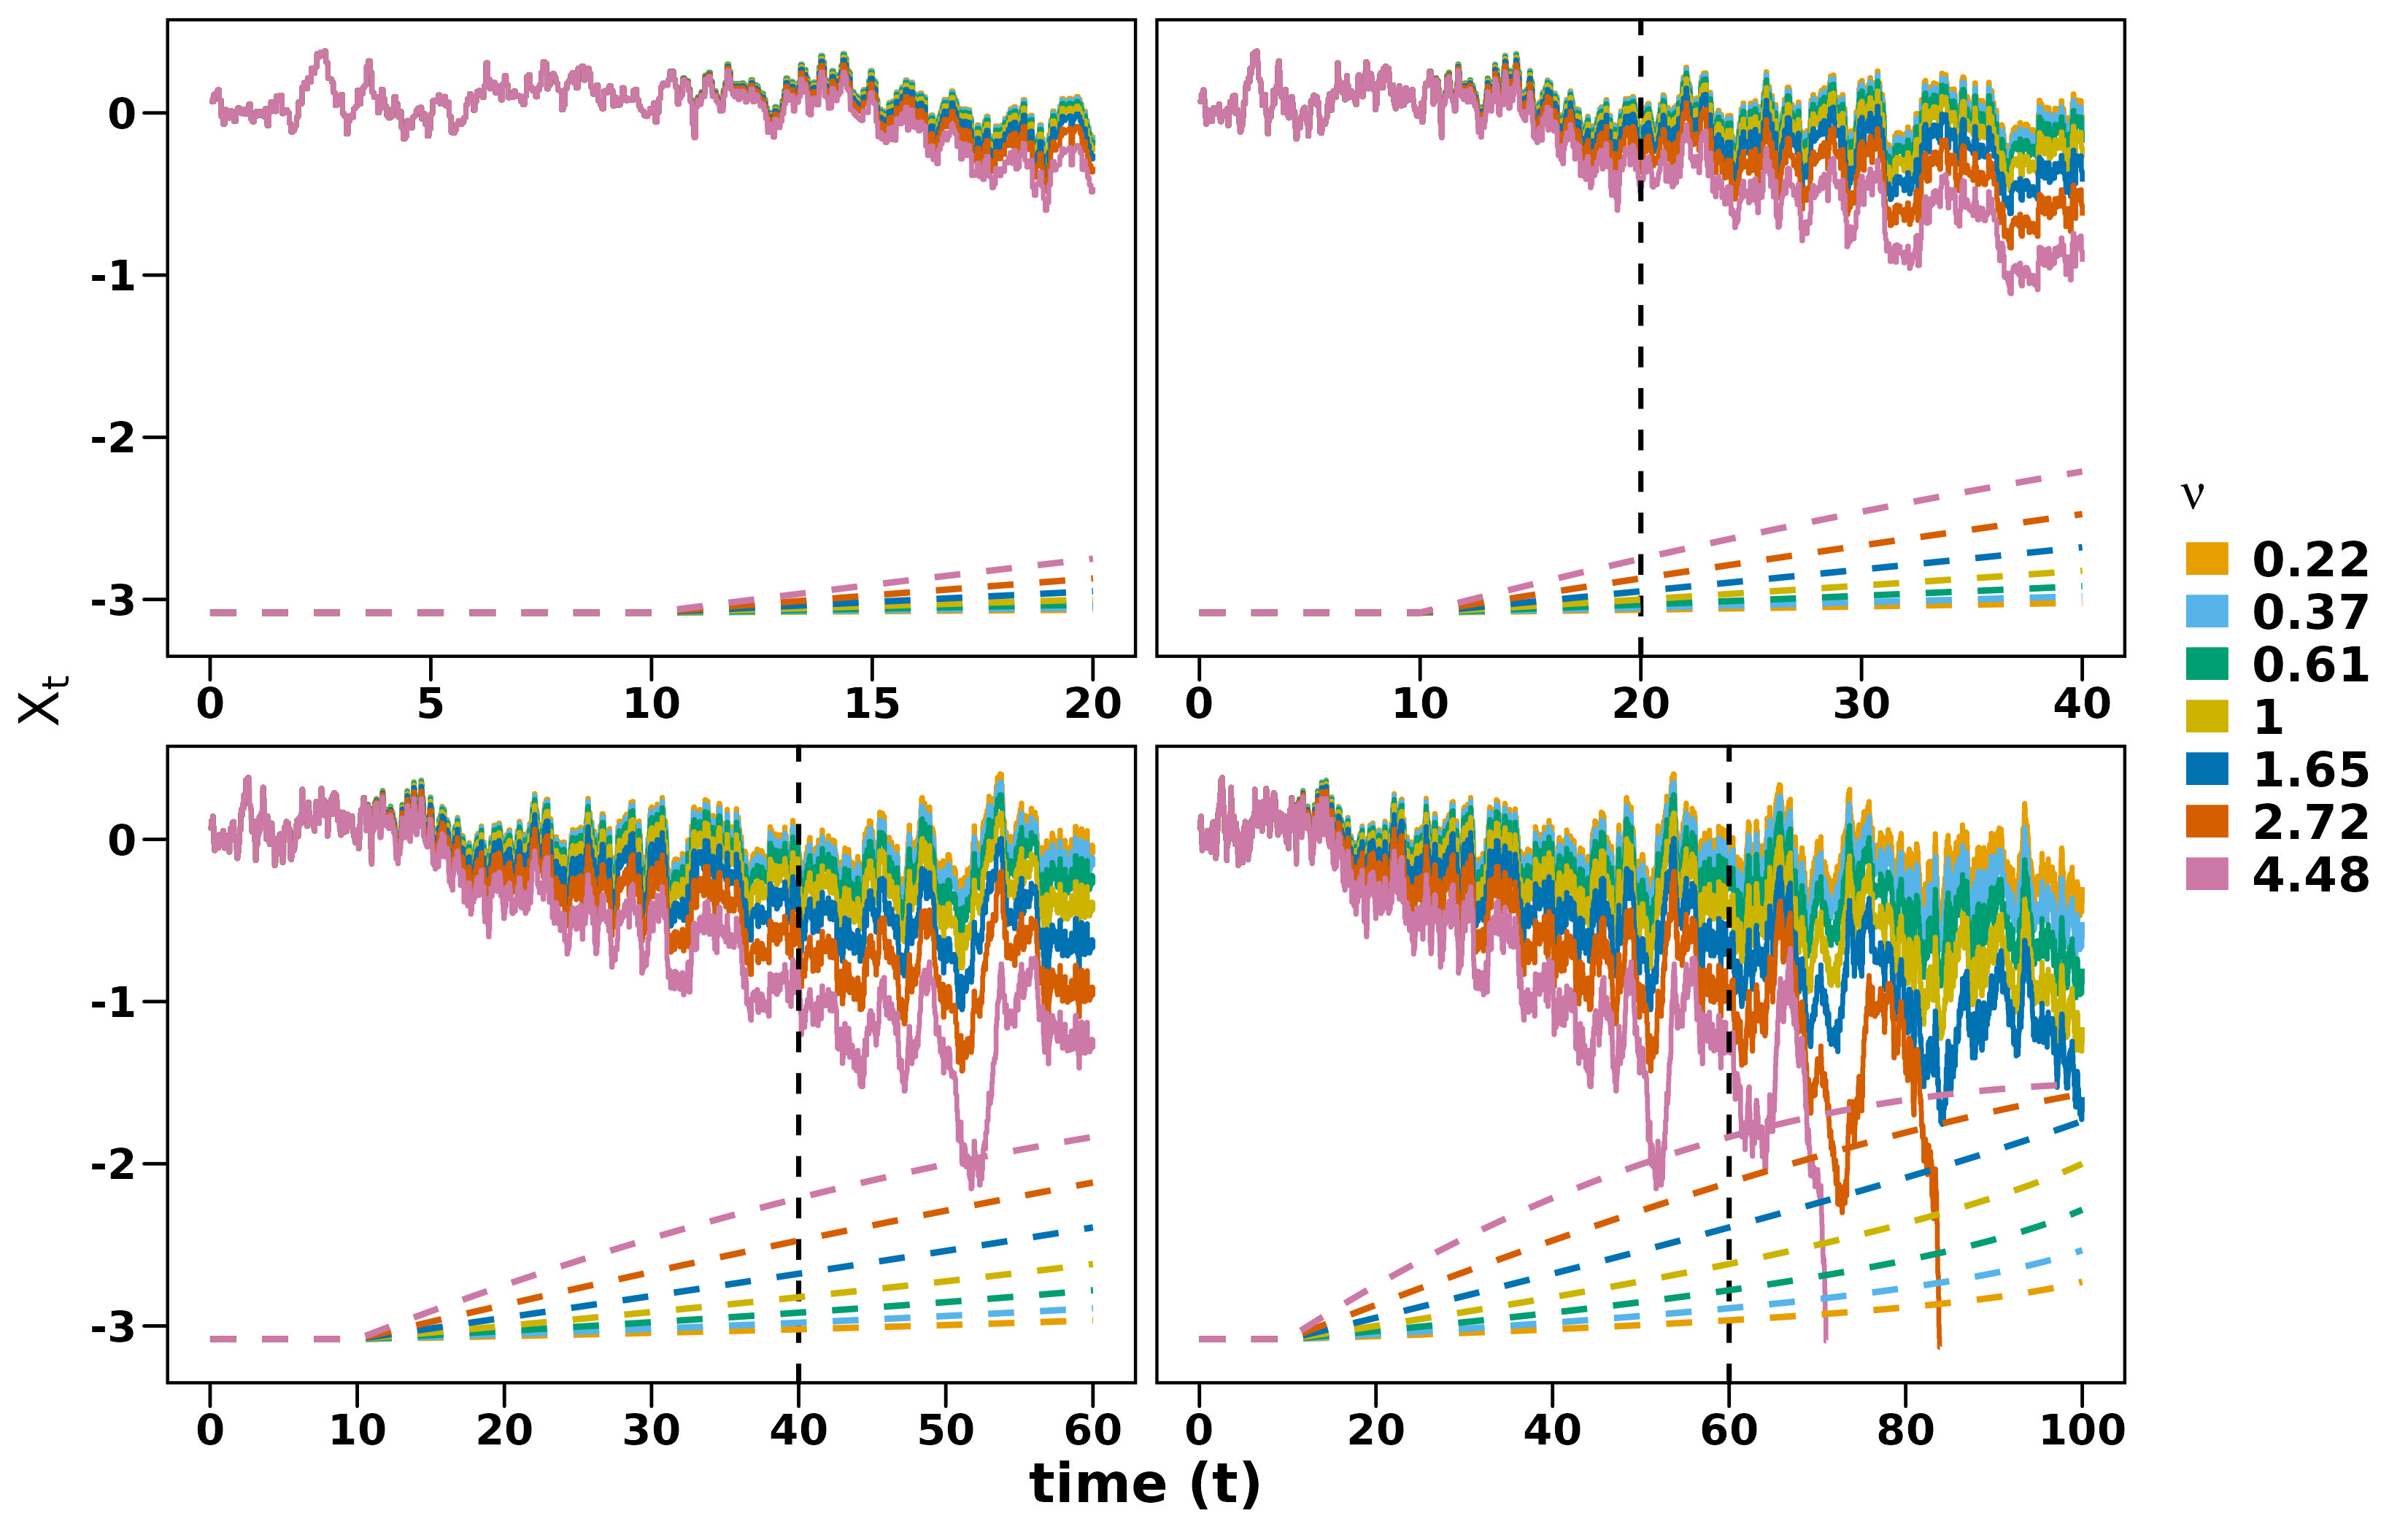
\includegraphics[scale = .13]{figures/mu_simulations_discussion_plot.jpeg}
    \caption{Sample paths for varying $\nu$ with the same realizations from the brownian motion cut at different points in time.}
    \label{figure:mu_simulations_discussion_plot}
    \end{center}
\end{figure}\\
This example is of course constructed for the sake of illustration and the following points might not always hold. However, Figure \ref{figure:mu_simulations_discussion_plot} is a clear example of some of the difficulties that can arise with regard to the estimation of the $\nu$-parameter. In each facet, the vertical dashed line marks the point in time up to which the facet before it ran. The colored dotted lines in the plots are the unstable fixed points that if crossed before the tipping point most likely result in the process experiencing noise-induced tipping. When this happens we can no longer predict a bifurcation tipping. Furthermore, due to noise-tipping the process is no longer close to the stable fixed point, whence there is no information about $\nu$ in the samples. All this means that in some cases, we need there to be enough time to the bifurcation point so we have not tipped because of noise yet.

Conversely, we still need to have quite a long series of observations within the dynamic part of the process to be able to distinguish between the paths. We are only 10 units of time within the dynamic part in the upper left facet in Figure \ref{figure:mu_simulations_discussion_plot}, and we can barely tell the sample paths coming from very different values of $\nu$ apart. That is at least visually.

All in all, we might need more sophisticated optimization methods than \code{optim} to have success with estimating $\nu$. An option here we have not mentioned yet is using automatic differentiation (AD). AD has lately been made more easily applicable in \code{R} via the \code{torch} framework \cite{torch}. Another option is to develop our numerically founded objectives even further, albeit its possibilities of finding fixed points for a range of values $t$ as required in the dynamical part are quite limited without some a priori given assumptions about the evolution of these fixed points. Luckily this is exactly what we have in the model, i.e. we have the specific form of $\lambda$ used in (\ref{eq:fixedPoint}). This allows us to potentially create a sub-optimization problem: Though, we do not observe $\lambda$ directly, the sample paths should be close to the fixed point on average; assuming that the process does not tip due to noise, of course. With this, we could perhaps use non-linear least squares to regress $\mu_t$ on the samples. We did experiment a bit with this with the method \code{stats::nls} but only got limited success. Solving the non-linear least squares at every iteration of the optimization is rather computationally expensive and it was quite error-prone: At some iterations, the \code{stats::nls} failed due to other parameters such as $A$ making the problem infeasible. To avoid this we could for instance adopt the penalization of $A$ used in \cite{Ditlevsen2023}.\\\\
Another thing we tried was making the numerical Strang method purely numerical. That is, it should be implemented such that all the computations are done by the program and the user merely provides the data, the specific model one wants to fit and the usual values required for optimization. In other words, the user should not need to provide the Lamperti SDE nor even the Lamperti transform (\ref{eq:lampertiDefinition}) here. The only thing the objective would need to know is the diffusion coefficient of one's model. To achieve an estimator from this, the method must construct the Lamperti transform etc. numerically and then do the same steps as the other numerical Strang method does. We actually managed to implement a prototype of this. Yet, the computational speed of the method became the bottleneck of development; it took too long to evaluate the likelihood even once for the method to ever be viable. Now, a popular raison d'être of numerical methods is that they allow us to use complex estimators without going through extensive calculations. And while simplifying the calculations necessary down to nothing whatsoever would be ideal, the method as is still provides a significant reduction in number of manual computations needed. Furthermore, it is uncertain if we would be able to match the results shown in Figure \ref{figure:ARE_dist_linear_noise} or \ref{figure:ARE_dist_numeric_F_diffusion}, if we automated the calculations further. In addition, one could argue that it is to be expected that a user wanting to apply these methods would be able to find the Lamperti transform and compute the Lamperti SDE with Itō's formula, which is all the numerical Strang based method requires. This further motivates keeping the numerical Strang method as it is.\\\\
We already touched on the idea of using the Strang splitting scheme to approximate the score function. Now, a third way to use this scheme could be to construct martingale estimation equations for stochastic differential equations that are more complicated than the Pearson diffusions, e.g. for the dynamic part of the process. As with our idea of using Kessler's method on the stochastic differential equation in the splitting, this method does not use the Lamperti transform. To see what we mean by this, consider the square root-based dynamical part of the saddle-node normal form model
\begin{align}
    \mathrm{d}X_t = -(A(X_t - m)^2 + \lambda_t)\mathrm{d}t + \sigma\sqrt{X_t}\mathrm{d}W_t. \label{eq:squareSplittingDiscussion}
\end{align}  
A direct splitting around the fixed point of this process, which alse can be found in section \ref{subsubsec:squarerootDynamic} is
\begin{align}
    \mathrm{d}X_t^{[1]} &= -\alpha(\lambda)\left(X_t^{[1]} - \mu(\lambda)\right)  \mathrm{d}t + \sigma \sqrt{X_t^{[1]}} \mathrm{d}W_t, \label{eq:squareRootSplit1_discussion} \\
    \mathrm{d}X_t^{[2]} &= - A \left(X_t^{[2]} - \mu(\lambda)\right)^2 \mathrm{d}t, \label{eq:squareRootSplit2_discussion}
\end{align}
with $\alpha(\lambda) = 2\sqrt{-A\lambda_t}$ and $\mu(\lambda) = m + \sqrt{-\frac{\lambda_t}{A}}$. This gives us is an SDE (\ref{eq:squareRootSplit1_discussion}), for which we can construct martingale estimation equations. For the Strang composition, we recall that based on Figure \ref{figure:StrangAndLieTrotterPlot} the flow is a non-linear transform of the solution to the SDE (\ref{eq:squareRootSplit1_discussion}). So constructing the estimation equations for the whole flow is a matter of using a result about the relationship between eigenfunctions, $p_n(x)$ and eigenvalues $\lambda_n$ for a process such as $X_t^{[1]}$ and transformations of that process with functions such as $\varphi_2$. It turns out \cite[remark on p. 41]{StatisticalMethodsForSDE} that in this case the eigenfunctions are $p_n\left(\varphi_2^{-1}(x)\right)$, whereas the eigenvalues remain the same. Still, it is unlikely that we would be able to get the conditional mean and variance of the flow needed for (\ref{eq:approximatelyOptimalMartingale}) from these eigenfunctions and eigenvalues, so in the remaining calculations one has to use a few more results from the theory of estimation equations than what has been presented here.
\newpage
\subsection{Tipping of the AMOC}
Taking Figure \ref{figure:surival_curve_taus} and Table \ref{table:tipping_quantiles} as our starting points of the discussion, it is clear that all the models indicate tipping to be \textit{more} than likely within the next 140 years. By "likely" we understand the 66\% confidence interval used by the Intergovernmental Panel on Climate Change \cite{Ditlevsen2023} and across all models and fingerprints there is at least an $83.5\%$ chance of tipping occurring before the end of the year $2169$. What specific range of years the tipping of the AMOC is likely within varies a bit according to the different models. Still, all the \textit{estimates} from the data lie within medio 21st century and primo 22nd century signifying some form of overall agreement.\\\\
We did not investigate penalization on the models, but it would be interesting to implement some sort of penalization on $A$ into the $t$-diffusion-based model as well. To get an idea of how this could affect the estimates of the tipping time consider pairs of estimates of tipping year and $A$ stratified after model.
\begin{figure}[h!]
    \begin{center}
    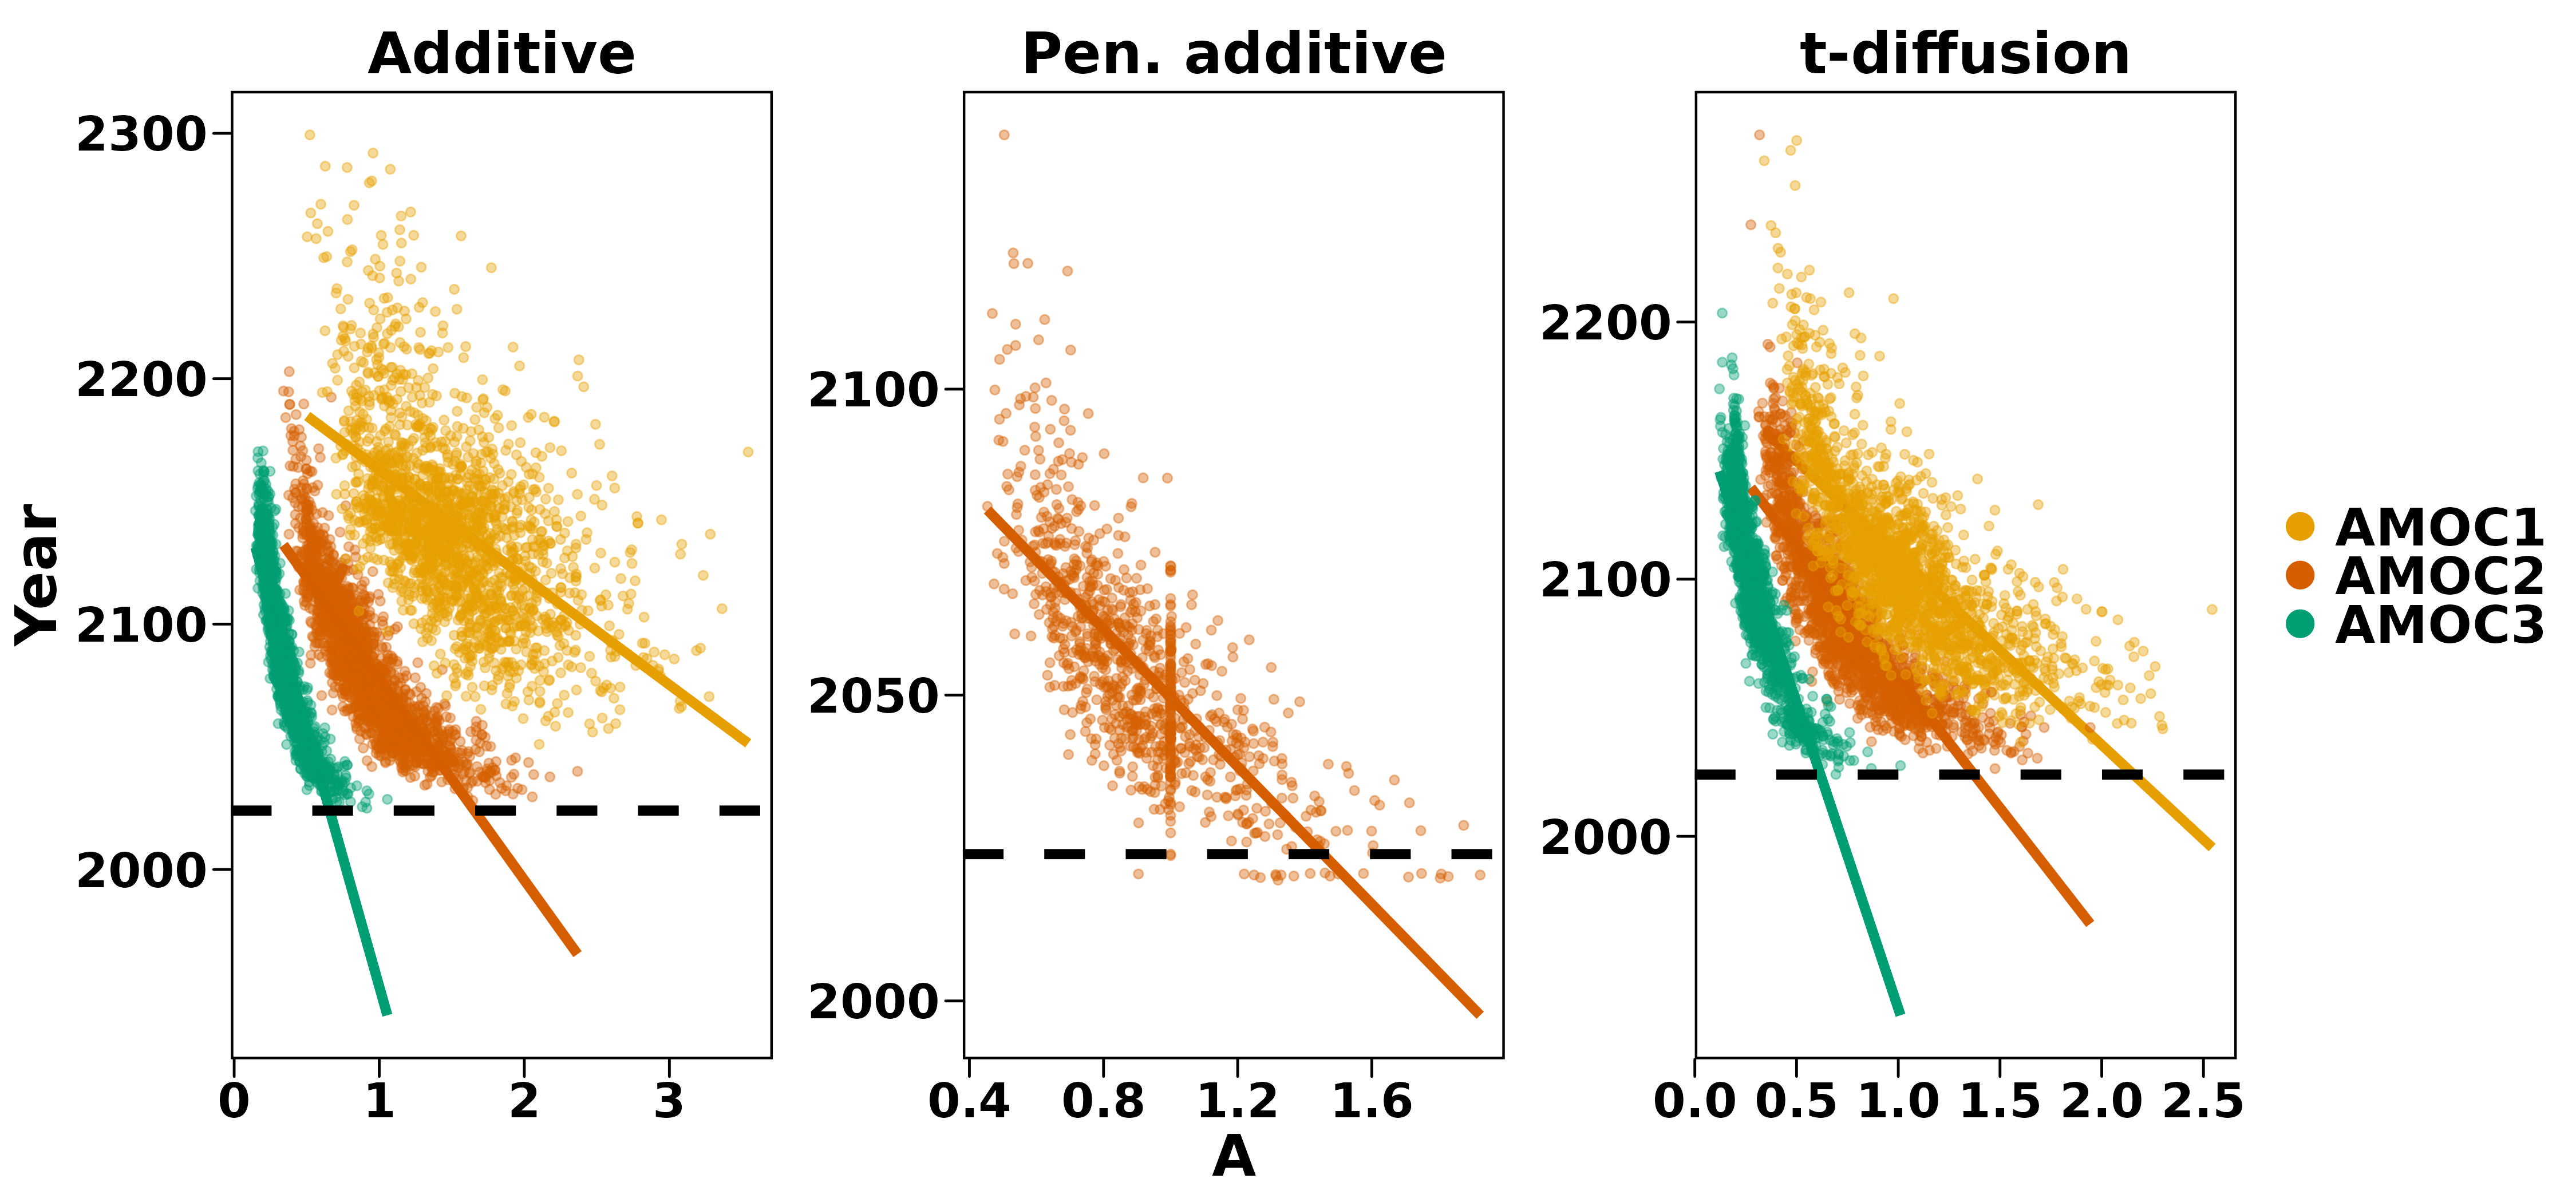
\includegraphics[scale = .082]{figures/correlation_between_A_and_tau_plot.jpeg}
    \caption{Pairs of estimates of tipping year and $A$ grouped by model and fingerprint}
    \label{figure:correlation_A_and_tau}
\end{center}
\end{figure}\\
The straight lines in the graphs are linear normal models fitted to the stratified samples they share color and facet with. In all cases, there is a strong negative correlation between the estimate of $A$ and -the tipping year; small values of $A$ tend to be have tipping estimates far in the future and vice versa. Indicating that if we want to avoid heavy-tailed estimators of $\tau_c$ we might want to penalize values of $A$ below 1 as done in the paper.

However, as seen in the graph in Figure \ref{figure:correlation_A_and_tau} the specific form of penalization creates a bias towards $A = 1$. Actually, one could argue that the penalizations might have hurt the optimization somewhat. Note the clear cluster of points forming around $A = 1$ in the middle graph of Figure \ref{figure:correlation_A_and_tau}. This is likely a result of penalization of values below $A$ resulting in the optimization pushing the parameter values \textit{really} close to $A = 1$. In fact, a closer investigation reveals that the penalization results in $12.4\%$ of estimates of $A$ being closer than $0.0005$ units away from $1$, whereas the proportion of estimates of $A$ with an absolute distance of just $0.000025$ to $1$ is still $7.9\%$. While we of course expect the distribution to shift towards $1$ for values that would have been much smaller than $A = 1$, so many values this close to $1$ is a bit concerning and could indicate that there is something unintended going on.

Yet, looking at the source code nothing particular from the objective function has stood out in this regard and the hyperparameter used in the penalization is picked carefully with cross-validation. One thing to note in the penalization itself is that the initial value of $A$ is 1. This could cause many estimates around the value 1, if the optimization algorithm is not explorative enough. As mentioned, the paper uses the \code{Nelder-Mead} algorithm for optimization. This algorithm is generally considered more exploitative than explorative. While this exploitive nature ensures we do not get the extreme estimates that our methods sometimes suffer from, there is the risk of getting stuck in local minima. To see if this is the case here, we implement a tracer into the objective function. This allows us to retrieve the parameters and objectives at every iteration and potentially diagnose any problems. We sketch the trace of each of the parameters, where we have used the penalized additive model on the AMOC2 fingerprint with starting values $A = 1$ and $\tau_c = 100$. 
\begin{figure}[h!]
\begin{center}
    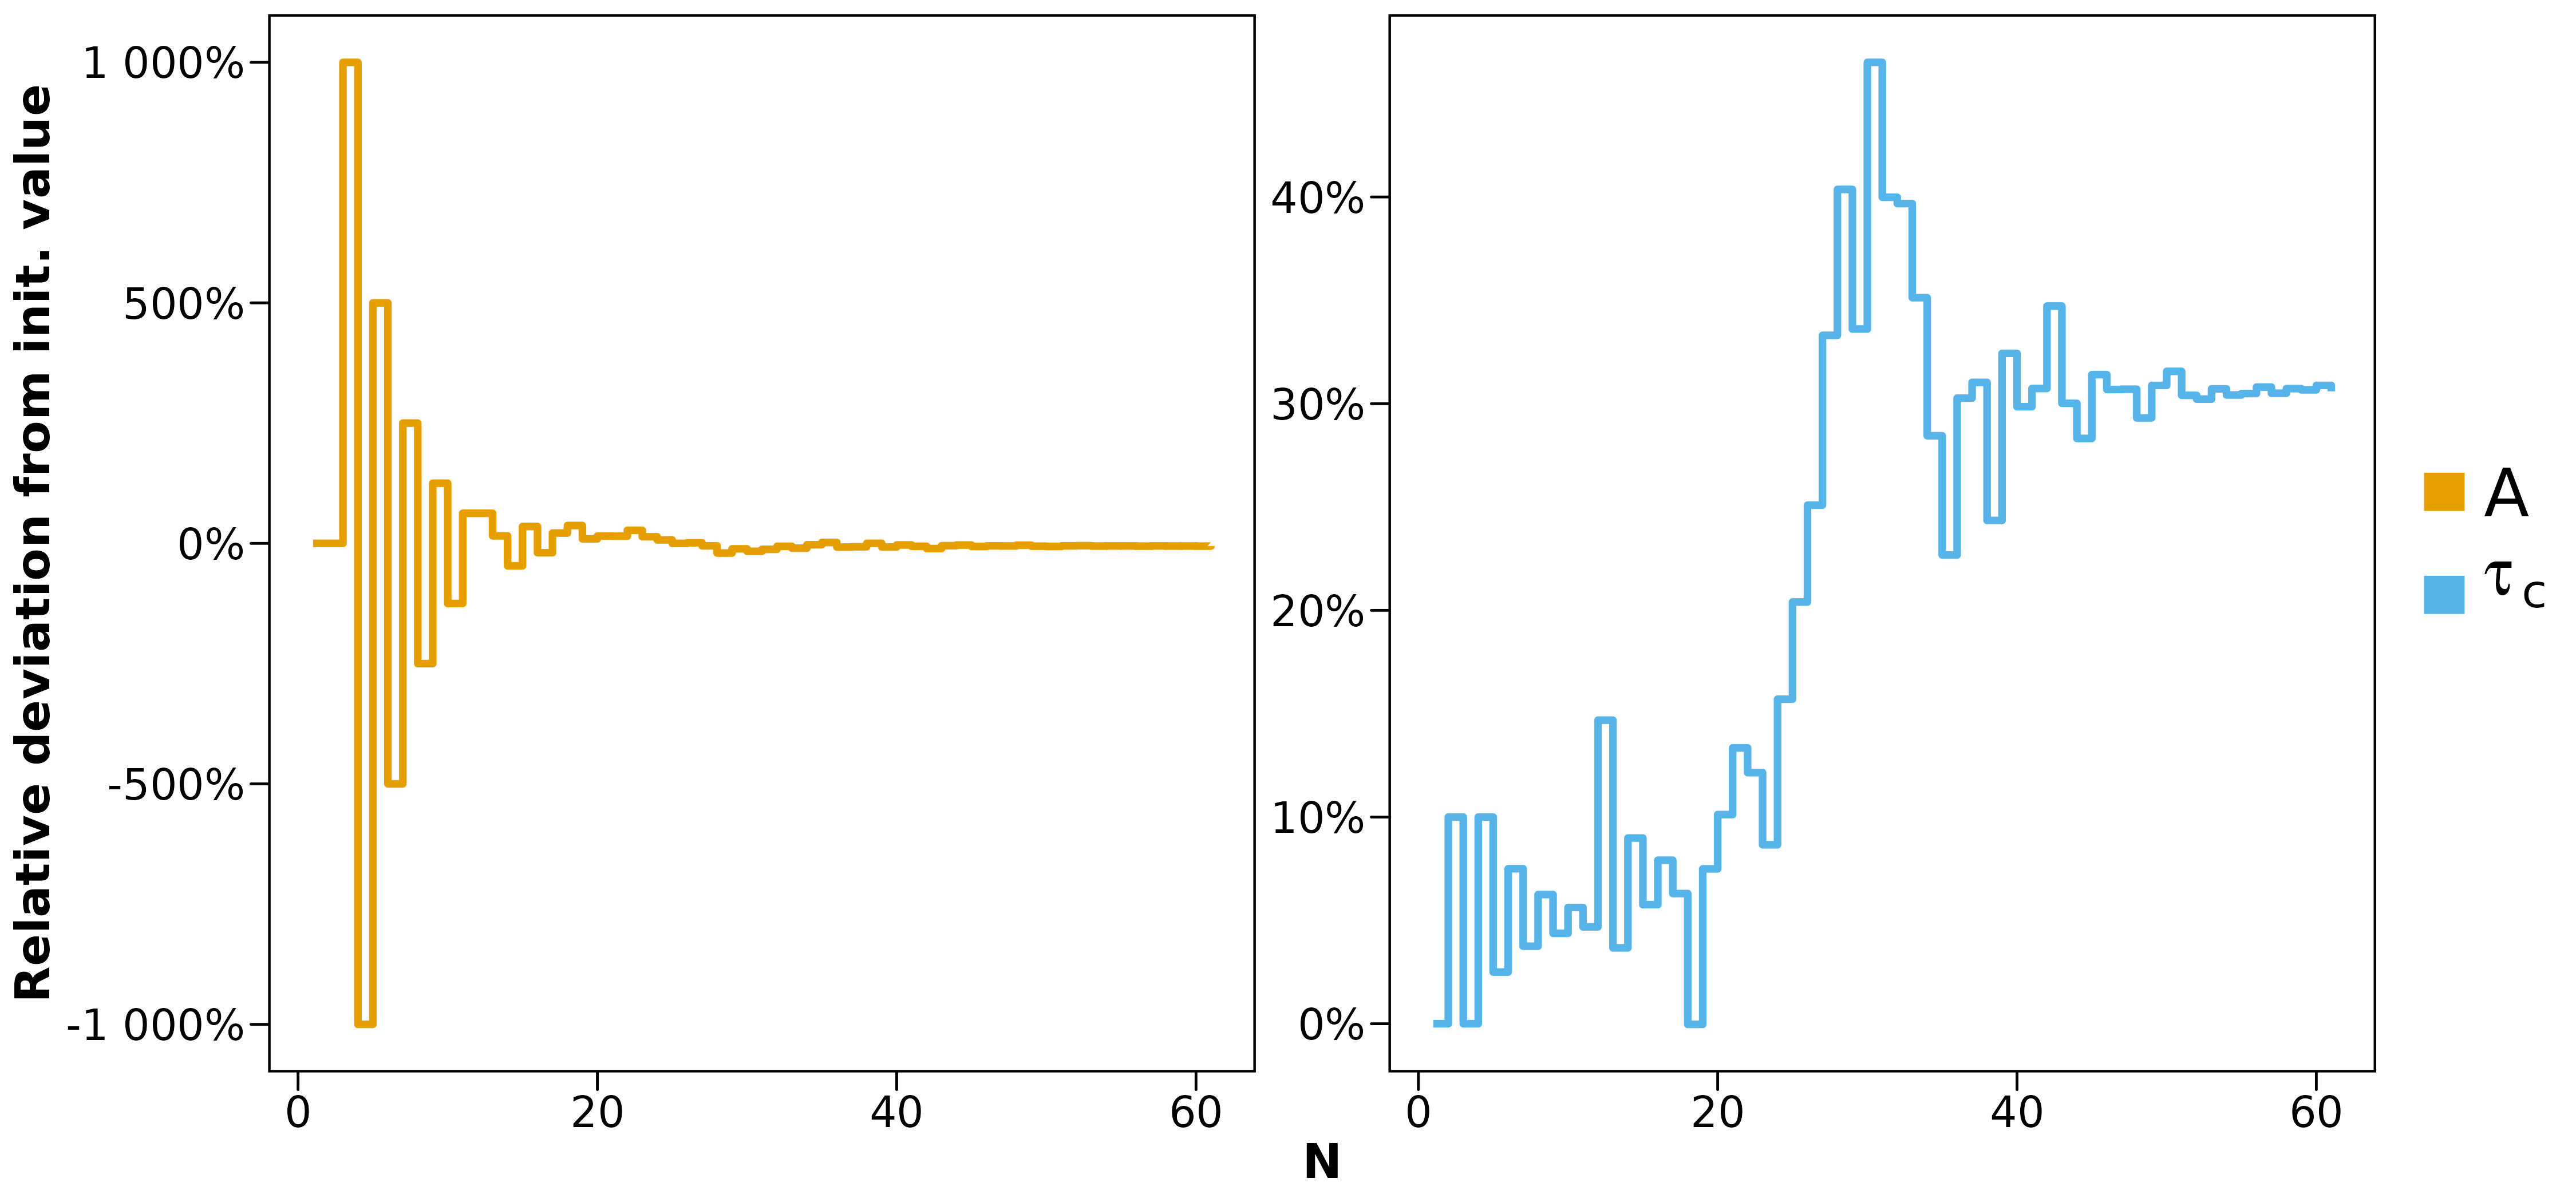
\includegraphics[scale = .075]{figures/trace_plot.jpeg}
    \caption{Trace plot of parameter values at each step of the optimization showing the relative deviation from the initial values $A = 1$ and $\tau_c = 100$.}
    \label{figure:trace_plot}
\end{center}
\end{figure}\\
As we clearly see from the trace, there is no lack of exploration of the $A$-parameter in this example; the optimizer searches among parameter values far away from the starting value. The same thing can be said about $\tau_c$ though its trace appears more guided overall. Of course, this is only one trace and we would need to examine more traces to reject this potential problem more confidently. On the other hand, the underlying cause might just be the fact that the penalty is applied at a discrete level $A<1$; this could potentially push values of $A$ moderately close to 1 closer, such that many estimates would be quite close in this way.

Regardless of whether it is caused by something undesired, having many values of $A$ around $1$ limits the range of values of the tipping, shifting $\tau_c$ in the specific direction as argued by the negative correlation in Figure \ref{figure:correlation_A_and_tau}. Again, there is nothing inherently wrong with the correlation of the estimates, but it becomes an issue, if there is something problematic in the optimization phase such as the potential problem illustrated here. And although we have not been able to establish the exact underlying cause, there could be reasons to believe that something in the optimization should be changed. Whether that is the type of penalization, the penalization altogether or something completely different, we do not answer here.

Apart from this, we should also mention that we discovered a minor bug in the implementation of the objective function for the dynamic part of the additive model that is in the supplementary material of the paper \cite{DitlevsenSupplementary}. The bug has since been corrected and although the estimates are a bit different, it has been checked that the distribution of the tipping time stays roughly the same after the correction. This means the arguments and comparisons made with results from the paper still hold. For this reason, we do not redo all the computations to recreate the distributions of \cite{Ditlevsen2023}. To this end, it is worth mentioning that there are other minor differences in the choices made between the estimation methods of the paper and this project such as whether $\sigma$ or $\sigma^2$ is estimated, what optimization algorithm is used, whether $A$ is allowed to be negative etc.
These differences can compound making the results quite different overall. 

With this in mind, we get $2054$ for the tipping time with the exact penalization used in the paper applied in our objective function for the additive model. This is rather close to the original result, confer Table \ref{table:tipping_quantiles}, which further justifies the use of the results from the paper in spite of the minor discrepancies. Again, the result we just presented comes with the caveat that the implementation from the paper might not agree completely and it might have been a bit naïve of us to select the exact same penalization value for the optimization and not determine it via cross-validation ourselves. However, it is done in the way to try and ensure some overall comparability to the original implementation.\\\\
Returning to the selection between the two models; in our initial discussion (below Figure \ref{figure:OU_t_diffusion_QQ_plot}) we favored the $t$-diffusion model as its uniform residuals resembled that of the standard Gaussian better overall — suggesting a better fit. Confer Table \ref{table:tipping_quantiles} the models agree on the estimated tipping times and their confidence intervals — for the most part. On the AMOC2 data, they are almost in complete agreement. Interestingly, the additive model generally puts tipping later on the AMOC1 fingerprint and earlier on the AMOC3 in comparison with the $t$-diffusion-based model. A strength in the $t$-diffusion model here is that it is more robust against the choice of fingerprint than the additive model; this can also be seen by how close the survival curves in Figure \ref{figure:surival_curve_taus} are.

Generally, we have argued for the $t$-diffusion model in our own work. It seems to provide a better fit overall, while also ensuring robustness without even needing a tuning of hyperparameters for penalization. However, with the limited tools we have to differentiate between the models, one could argue that the real significance of using multiple different stochastic terms with the same deterministic drift, as we have with the construction \ref{eq:standardStochasticForm}, is that it adds a different layer to the robustness analysis. If one can illustrate an effect in the deterministic part of a stochastic differential equation using several models with different diffusion terms, it would strengthen the belief in our estimates as it is clearly less dependent on model selection. We succeeded in doing so with two of our models, though, preferably we would like to be able to apply other models as well. However, as we noted only two of the models we have shown are applicable to data with negative observations. There might be ways to adapt the diffusion terms in the other models to extend them to the real numbers, while still keeping their structure. Another solution could be to use some monotone map from the reals onto the positive real numbers, e.g. the exponential function, on the data. As our domain knowledge on climate physics is somewhat limited, we refrain from doing so here.\\\\
A completely different option is instead of letting the ramping of the bifurcation parameter, $\lambda_t$ depend on time in a way that bifurcation inevitably occurs, we could model the bifurcation parameter using, say, a linear normal model. This allows us to use covariates e.g. the $\mathrm{CO}_2$ levels in the Earth's atmosphere. A specific model that we have thought about is the following
\begin{align}
    \lambda_x= \beta_2 x + \beta_1, \label{eq:alternativeLambda}
\end{align}
where $x$ is the logarithm of the global mean $\mathrm{CO}_2$ in the atmosphere. The objective here would be to estimate the parameters $\beta_1$ and $\beta_2$; this would allow us to find the critical value by solving $\lambda_x = 0$ for $x$, i.e. $\hat{\lambda_c} = -\frac{\hat{\beta_1}}{\hat{\beta_2}}$; giving us the $\mathrm{CO}_2$ level at which tipping occurs instead of the point in time. A minor point to note here is that $\hat{\lambda_c}$ is not a very well-behaved estimator. Being the ratio of two Gaussian variables it has for instance no mean. Other variations of a model with covariates could be an extension of the linear regression ramping model, where we introduce a parameter like $\nu$ in an exponent analogously to (\ref{eq:lambdaRampDefinition}), turning the sub-problem into a non-linear regression problem. \\\\
Regardless on the exact model one ends up using, it would not only be a model that is quite different to estimate in, it would also shift the perspective on the tipping model somewhat. In the \textit{time to tipping} type models there are of course the built-in assumption in the ramping (\ref{eq:lambdaRampDefinition}) that the development in the past continues going forward and the tipping time should of course be taken with this caveat. Though, what exactly drives the evolution of $\lambda_t$ is difficult to reason about, so it is hard for us to intuitively see if the evolution in the future follows the expected path or deviates. On the other hand, a tipping $\mathrm{CO}_2$ value could be easier to communicate and we can easily measure if the concentration of $\mathrm{CO}_2$ in the atmosphere is below the threshold. 

Furthermore, the two models invite us to think in completely different ways in the first place: That ramping does not necessarily continue can be hard to remember for a layperson; in that light, a tipping time type model seems like a crystal ball predicting an inevitable event in the future. On the other hand, with the \textit{tipping level} type model, it is easy to fall into the trap of seeing tipping as a phenomenon that necessarily occurs at specific $\mathrm{CO}_2$ levels. That is assuming a form of causality, the model does not let us reason about. However, the tipping level type excels in encouraging us to think about the system in a structured manner. One could for instance ask very concrete questions such as what levels of $\mathrm{CO}_2$ we should avoid for it to be "likely" that the system does not reach a tipping point. \\\\
Finally, if we had both types of models they could, and arguably should, be used in conjunction. With them, we could check if the estimated time of tipping aligns well with our current $\mathrm{CO}_2$ projections. That is, does the projected time for our reaching the critical $\mathrm{CO}_2$ level agree with the critical time in the tipping time type models? In the confirming case, this would be an excellent tool to make the estimates even more convincing. If they do not agree, we are left with interesting question as to why this could be the case.

\subsection{Conclusion}
In sum, we have proposed two types of natural extensions to the stochastic normal form of the saddle-node bifurcation model. Simulation studies where we put realistic limitations on the knowledge of the initial parameters have shown that we so far can estimate the parameters of all six variations of the model fairly well as long as we omit the $\nu$-parameter. It was somewhat unsatisfactory that we could not get the estimation of the $\nu$-parameter to work in cases, where we initialized the parameter in $1$; corresponding to assuming the simpler ramping model from previous work. However, we did reflect on alleys to go down which could lead to a more numerically stable method that could allow the estimation of $\nu$.\\\\
At the same time, we managed to contribute with new insights into the potential tipping point in the Atlantic Meridional Overturning Circulation. Using the additive model without penalization and a model based on the diffusion term from the $t$-diffusion to estimate the tipping point of this system we found results that are in the same range as what was found in the original work on the subject, albeit we have slightly more conservative estimates — putting tipping to be likely within the next 140 years across all models and fingerprints. In general, we saw a much heavier tail than the original estimates of the year of tipping. However, for most models and fingerprints we saw it was likely within the next 100 years, which aligns well with the previous work. Finally, we mentioned interesting paths that future research may take and proposed and reflected on the general ease of interpretability of these models. 
\newpage
\bibliography{refs.bib}
\newpage
\appendix
\section*{Appendix}\label{Appendix}
\section{Source code}
The source code for this project, licensed under the MIT License, is hosted on \href{https://github.com/Gantzhorn/Thesis}{Github}. In the repository the source code can be found in the \textit{"source\_code"}-directory. To recreate the main results from the thesis run the \code{R}-script: \textit{"main.R"}. For the code itself refer to the other \code{R}-files in the same directory. Apart from the code these also includes information about the code as well as examples on how to actually run it. 
\section{Simulation Methods}\label{appendix:simMethods}
This section focuses on constructing the simulation schemes that support the analytical work presented in this thesis. We considered the Euler-maruyama - as well the Milstein scheme. However, as the processes are quite non-linear our final choice was the Scalar weak order 2.0 Itô–Taylor method \cite[algorithm 8.5]{Srkk2019}. In the general setup we simulate $X_{t_0},X_{t_1},\dots, X_{t_N}$ according to the schemes by sampling $N$ random variables $\Delta W_{t_k}\sim\mathcal{N}\left(0, \Delta t_k\right)$. Note that we let $X_{t_0} = \mu_0$, i.e. mean-reverting parameter in the stationary parts of the processes.
\noindent \textbf{Additive noise}\\
Invoking \cite[algorithm 8.5]{Srkk2019} we get the scheme
\begin{align}
    X_{t_{k + 1}} &= X_{t_k} - \left(A(X_{t_k} - m)^2 + \lambda_{t_k}\right) \Delta t_k + \sigma \Delta W_{k} \nonumber \\&-  A \left(X_{t_k} - m\right)\sigma \Delta W_k \Delta t_k\nonumber \\
    & + \left(A\left(X_{t_k} - m\right)\left(A\left(X_{t_k} - m\right)^2 + \lambda_{t_k}\right) - \frac{A \sigma^2}{2}\right)\left(\Delta t_k\right)^2 \label{eq:OUSim}
\end{align}
\\
\textbf{Square-root noise}\\
For the square-root based process the algorithm gives 
\begin{align}
    X_{t_{k + 1}} &= X_{t_k} - \left(A(X_{t_k} - m)^2 + \lambda_{t_k}\right) \Delta t_k + \sigma \sqrt{X_t} \Delta W_{k}\nonumber\\ &+ \frac{1}{4}\sigma^2 \left(\Delta W_k^2 - \Delta t_k\right)     - A\left(X_{t_k} - m\right)\sigma \sqrt{X_{t_k}} W_k \Delta t_k
    \nonumber\\
     &+ \left(A\left(X_{t_k} - m\right)\cdot \left(A\left(X_{t_k} - m\right)^2 + \lambda_{t_k}\right) - \frac{A\sigma^2 X_{t_k}}{2}\right)(\Delta t_k)^2 \nonumber\\
    &- \frac{1}{4\sqrt{X_{t_k}}}\left(\sigma\left(A\left(X_{t_k} - m\right)^2 + \lambda_{t_k}\right) + \frac{1}{4}\sigma^3\right) \left(\Delta W_k \Delta t_k\right)
\end{align}
\\
\textbf{Linear noise}\\
With linear noise we get the simulation scheme
\begin{align}
    X_{t_{k + 1}} &= X_{t_k} - \left(A(X_{t_k} - m)^2 + \lambda_{t_k}\right) \Delta t_k + \sigma X_t \Delta W_{k} \nonumber \\ &
    + \frac{1}{2}\sigma^2 X_{t_k}\left(\Delta W_{k}^2 - \Delta t_k\right) -A(X_{t_k} - m)\sigma X_{t_k} \Delta W_k\Delta t_k \nonumber\\
    & + \left(A\left(X_{t_k} - m\right)\left(A\left(X_{t_k} - m\right)^2 + \lambda_{t_k}\right) - \frac{A\sigma^2X_{t_k}^2}{2}\right)(\Delta t_k)^2 \nonumber \\
    &- \frac{\sigma}{2}\left(A\left(X_{t_k} - m\right)^2 + \lambda_{t_k}\right)\left(\Delta W_{k}\Delta t_k\right).
\end{align}
\\
\textbf{Skew t-distribution}\\
With the skew t distribution as the Stationary distribution of the non-dynamic part of the process we get the following scheme
\begin{align}
    X_{t_{k + 1}} &= X_{t_k} - \left(A(X_{t_k} - m)^2 + \lambda_{t_k}\right) \Delta t_k + \sigma \sqrt{\left(X_{t_k}^2 + 1\right)} \Delta W_{k} \nonumber\\
    &+ \frac{\sigma^2}{2}X_t \left(\Delta W_{k}^2 - \Delta t_k\right) - A\left(X_{t_k} - m \right)\sigma\sqrt{\left(X_{t_k}^2 + 1\right)}\Delta W_{k}\Delta t_k \nonumber\\
    &+ \left(\left(A\left(X_{t_k} - m \right)^2+\lambda_{t_k}\right)\left(A\left(X_{t_k} - m \right)\right) - \frac{A\sigma^2}{2}\left(X_t^2 + 1\right)\right)\left(\Delta t_k\right)^2 \nonumber\\
    &-\left(\sigma X_{t_k}\left(A\left(X_{t_k} - m \right)^2 + \lambda_{t_k}\right) - \frac{\sigma^3}{2}\right)\frac{\left(\Delta W_{k}\Delta t_k\right)}{2\sqrt{X_{t_k}^2 + 1}}
\end{align}
\\
\textbf{F-distribution}\\
The model with the F-distribution as the stationary distribution in the non-dynamic part is sampled in the following manner
\begin{align}
    X_{t_{k + 1}} &= X_{t_k} - \left(A(X_{t_k} - m)^2 + \lambda_{t_k}\right) \Delta t_k + \sigma\sqrt{X_{t_k}\left(X_{t_k} + 1\right)}\Delta W_k \nonumber \\
    &+ \frac{\sigma^2}{4}\left(2X_{t_k} + 1\right)\left(\Delta W_k^2 - \Delta t_k\right) - A \left(X_{t_k} - m\right)\sigma \sqrt{X_{t_k}\left(X_{t_k} + 1\right)}\Delta W_k \Delta t_k \nonumber \\
    &+ \left(\left(A\left(X_{t_k} - m\right)^2 + \lambda_{t_k}\right)\left(A\left(X_{t_k} - m\right)\right) - \frac{\sigma^2A}{2}\left(X_{t_k}\left(X_{t_k} + 1\right)\right)  \right)\left(\Delta t_k\right)^2 \nonumber \\
    &- \left(\sigma\left(A\left(X_{t_k} - m\right)^2 + \lambda_{t_k}\right)\left(2 X_{t_k} + 1\right) + \frac{\sigma^3}{4}\right)\frac{\Delta W_k \Delta t_k}{4\sqrt{X_{t_k}\left(X_{t_k} + 1\right)}}
\end{align}
\\
\textbf{Jacobi-diffusion}\\
Basing the modelling on the jacobi diffusion yields a scheme
\begin{align}
    X_{t_{k + 1}} &= X_{t_k} - \left(A(X_{t_k} - m)^2 + \lambda_{t_k}\right) \Delta t_k + \sigma \sqrt{X_{t_k}\left(1-X_{t_k}\right)} \Delta W_{k} \nonumber\\
    &+ \frac{\sigma^2}{4}\left(1 - 2X_{t_k}\right)\left(\Delta W_k^2 - \Delta t_k\right) - A\left(X_{t_k} - m\right)\sigma \sqrt{X_{t_k}\left(1 - X_{t_k}\right)}\Delta W_k\Delta t_k \nonumber \\
    &+ \left(\left(A\left(X_{t_k} - m\right)^2 + \lambda_{t_k}\right)\left(A\left(X_{t_k} - m\right)\right) - \frac{\sigma^2A}{2}\left(X_{t_k}\left(1 - X_{t_k}\right)\right)\right)\left(\Delta t_k\right)^2 \nonumber \\
    &- \left(\left(A\left(X_{t_k} - m\right)^2 + \lambda_{t_k}\right)\sigma\left(1 - 2X_{t_k}\right) + \frac{\sigma^3}{2}\right)\frac{\Delta W_k \Delta t_k}{4\sqrt{X_{t_k}\left(1 - X_{t_k}\right)}} \label{eq:jacobiDiffusion}
\end{align}
\section{Derivation of Estimators}\label{sec:AppendixEstim}
In this section, we derive the estimators that have been employed throughout the thesis. For sake of readibility, we leave out some of the more lengthy algebraic manipulations
\subsection{The Ornstein-Uhlenbeck based model}\label{subsec:OUprocess}
This section introduces the estimators for the dynamical system with additive noise. This is the same model introduced in \cite[equation (1)]{Ditlevsen2023} barring the addition of the $\nu$-parameter.
\subsubsection{Stationary part}\label{subsubsec:OUprocessStationary}
In the stationary part of the process we may assume that the process behaves like an Ornstein-Uhlenbeck process. 
\begin{align}
    \mathrm{d}X_t = -\alpha_0\left(X_t-\mu\right) \mathrm{d}t + \sigma \mathrm{d}W_t.
\end{align}
Let $\rho = \exp\left(-\alpha_0\Delta t\right), \gamma^2 = \sigma^2/2\alpha_0$. This process has transition density \cite[equation (S3)]{DitlevsenSupplementary}
\begin{align}
    p\left(\Delta t, x_{i-1}, x_i;\theta\right) = \frac{1}{\sqrt{2\pi\gamma^2\left(1-\rho^2\right)}}\exp\left(-\frac{\left(x_i-x_{i-1}\rho - \mu\left(1-\rho\right)\right)^2}{2\gamma^2\left(1-\rho^2\right)}\right), \label{eq:OULikelihood}
\end{align}
which is a gaussian density with conditional mean and -variance
\begin{align}
    \mathbb{E}\left[X_i\middle|X_{i-1} = x_{i-1}\right] &= x_{i - 1}\rho - \mu\left(1-\rho\right),\\
    \mathrm{Var}\left(X_i\middle|X_{i-1} = x_{i-1}\right) &= \gamma^2\left(1-\rho^2\right).
\end{align}
Unfortunately, we cannot get closed form solution to all of the estimators from this. However, we can still maximize (\ref{eq:OULikelihood}) with respect to $\theta$ to get the MLEs. Alternatively, we can derive the score equations by taking the derivative of the log-likelihood, and numerically solve the non-linear equations we get from doing so. The score equations are present in \cite[p.1, bottom]{DitlevsenSupplementary}. To solve the equations, we use the $\code{nleqslv::nleqslv}$-method \cite{nleqslv}. For starting values in both methods we use the approximation for the MLE of $\mu$ in equation \cite[(S4)]{DitlevsenSupplementary} along with (S4),(S5) for $\rho, \gamma^2$, which are good closed form approximations of the MLEs.
\subsubsection{Dynamic part}\label{subsubsec:OUprocessDynamic}
This part of the estimation procedure has to do with the estimation of the parameters linked to the dynamic part of the process. Our estimation procedure mostly follows \cite{Ditlevsen2023}. We, of course, have the addition of the $\nu$-parameter. Additionally, \cite{Ditlevsen2023} uses regularization in the form of a penalization parameter that punishes values of $A$ significantly smaller than $1$; we do not explore this option here. Recall the dynamics for $t>t_0$
\begin{align}
    \mathrm{d}X_t &= -\left(A\left(X_t - m\right) + \lambda_t\right)\mathrm{d}t + \sigma \mathrm{d}W_t \label{eq:additiveDynamicPart},\\
    \lambda_t &= \lambda_0\left(1 - \frac{t - t_0}{\tau_c}\right)^\nu.
\end{align}
For this part of the process, we utilize the estimation method described in \cite{DitlevsenSupplementary}. The fixed point of the process is $\mu\left(\lambda\right) = \sqrt{-\frac{\lambda_t}{A}}$. Linearizing the process around this value yields the splitting
\begin{align}
    \mathrm{d}X_t^{(1)} &= -\alpha\left(\lambda\right)\left(X_t^{(1)} - \mu\left(\lambda\right)\right)\mathrm{d}t + \sigma \mathrm{d}W_t, \label{eq:additiveSDE}\\
    \mathrm{d}X_t^{(2)} &= -A \left(X_t^{(2)} - \mu\left(\lambda\right)\right)^2\mathrm{d}t. \label{eq:additiveODE}
\end{align}
We recognize the Ornstein-Uhlenbeck process in (\ref{eq:additiveSDE}), for which the solution is (\ref{eq:OU_solution}). Denote this flow $\varphi_{\Delta t}^{(1)}(x)$. Additionally, one can show that (\ref{eq:additiveODE}) is solved by 
\begin{align}
    \varphi^{(2)}_{\Delta t}(x) = \frac{\mu\left(\lambda\right)A\Delta t\left(x - \mu\left(\lambda\right)\right) + x}{A\Delta t\left(x- \mu\left(\lambda\right)\right) + 1}.
\end{align}
By the remark below \cite[equation (9)]{SplittingSchemes} the inverse of the flow is
\begin{align}
    \left(\varphi^{(2)}_{\Delta t}\right)^{-1}(x) = \varphi^{(2)}_{-\Delta t}(x) = \frac{\mu\left(\lambda\right)A\Delta t\left(x - \mu\left(\lambda\right)\right) - x}{A\Delta t\left(x- \mu\left(\lambda\right)\right) - 1},
\end{align}
and by computing the derivative directly
\begin{align}
    \frac{\partial}{\partial x} \left(\left(\varphi^{(2)}_{\Delta t}\right)^{-1}\right)(x) = \frac{1}{\left(A \Delta t\left(x-\mu\left(\lambda \right)\right) - 1\right)^2}.
\end{align}
Then the Strang splitting approximates the transition density of (\ref{eq:additiveDynamicPart}) by
\begin{align}
    \left(X_{t + \Delta t} | X_t = x\right) &= \left(\varphi^{(2)}_{\Delta t / 2}\circ \varphi^{(1)}_{\Delta t} \circ \varphi^{(2)}_{\Delta t / 2}\right) \label{eq:OU_dynamic_likelihood}
\end{align}
This is the transformation of gaussian with appropriate parameters for the mean and variance according to (\ref{linearSDEMean}) and (\ref{linearSDEVariance}) respectively, so we can get the pseudo-loglikelhood using the elements from above and the density transformation theorem. The maximizer of (\ref{eq:OU_dynamic_likelihood}) is then our estimate. 
\subsection{Square-root process}\label{subsec:squareroot}
In this section we introduce the estimators for the model that is based on the square-root process. The estimators for the dynamic part of the process are unlike the ones from the model with additive noise that we showed in \ref{subsec:OUprocess} completely novel
\subsubsection{Stationary part}\label{subsubsec:squarerootStationary}
In the stationary part we assume the process can be modelled by the square-root process
\begin{align}
    \mathrm{d}X_t &= -\alpha_0\left(X_t - \mu_0\right)\mathrm{d}t + \sigma \sqrt{X_t} \mathrm{d}W_t. \label{eq:squarerootAppendix}
\end{align}
We first introduce estimators based on the Strang splitting scheme, and then we consider an estimator based on martingale estimating equations.\\\\
\noindent \textbf{The Strang-based Estimator}\\
To obtain the strang estimator, we first use the lamperti transformation of (\ref{eq:squarerootAppendix}), which by table \ref{table:ergodicDiffusions} is $Y_t := 2\sqrt{X_t}$. To confirm this and get the resulting SDE see
\begin{align}
    \mathrm{d}Y_t = - \frac{2}{Y_t}\left(\alpha_0 \frac{Y_t^2}{4} - \alpha_0 \mu_0 + \frac{\sigma^2}{2}\right)\mathrm{d}t + \sigma \mathrm{d}W_t, \label{eq:lampertiSquarerootAppendix}
\end{align}
by Itô's formula. Then, we use the heuristic from \cite[section 2.3 and 2.5]{SplittingSchemes}. First we calculate the fixed point of the drift. That is, we solve the equation
\begin{align}
    f(y) := - \frac{2}{y}\left(\alpha_0 \frac{y^2}{4} - \alpha_0 \mu_0 + \frac{\sigma^2}{2}\right) = 0
\end{align}
in terms of $y$. By the quadratic formula this is $y^* = \pm 2\sqrt{\frac{\alpha_0\mu_0 - \sigma^2 / 2}{\alpha_0}}$. In our case, however, $Y_t$ is non-negative by definition; thus we only want the positive solution. Therefore, we let the Ornstein-Uhlenbeck part be the linearization around the positive fixed point
\begin{align}
    \mathrm{d}Y_t^{[1]} &= -\alpha_0 \left(Y_t^{[1]} - 2\sqrt{\frac{\alpha_0\mu_0 - \sigma^2 / 2}{\alpha_0}}\right)\mathrm{d}t + \sigma \mathrm{d}W_t , \label{eq:squarerootStationarySplit1} \\
    \mathrm{d}Y_t^{[2]} &= \left(\frac{\alpha_0 Y_t^{[2]}}{2} + \frac{2\alpha_0 \mu_0 - \sigma^2}{Y_t} - 2\sqrt{\alpha_0\left(\alpha_0\mu_0 - \sigma^2 / 2\right)}\right)\mathrm{d}t. \label{eq:squarerootStationarySplit2}
\end{align}
As always, the deterministic ODE in (\ref{eq:squarerootStationarySplit2}) is the residual of (\ref{eq:lampertiSquarerootAppendix}) and (\ref{eq:squarerootStationarySplit1}).
Equation (\ref{eq:squarerootStationarySplit1}) represents an Ornstein-Uhlenbeck process, which with stepsize, $\Delta t$, has a gaussian flow with mean 
\begin{align}
    \mu_{\Delta t}(x) = \exp\left(-\alpha_0 \Delta t\right) \left(x - 2\sqrt{\frac{\alpha_0\mu_0 - \sigma^2 / 2}{\alpha_0}}\right) + 2\sqrt{\frac{\alpha_0\mu_0 - \sigma^2 / 2}{\alpha_0}}
\end{align}
and variance
\begin{align}
     \Omega_{\Delta t} = \frac{\sigma^2\left(1 - \exp\left(-2\alpha_0 \Delta t\right)\right)}{2\alpha_0}
\end{align}
\cite[(5), (6)]{SplittingSchemes}. We did not find an analytical solution to (\ref{eq:squarerootStationarySplit2}) unlike earlier. Instead, we rely  on the classical Fourth-Order Runge-Kutta Method \cite[p. 541]{numericalAnalysis} to find the flow. Nevertheless, we can denote these two flows $\varphi_{\Delta t}^{[1]}, \varphi_{\Delta t}^{[2]}$ respectively and the Strang splitting scheme is then the composition
\begin{align}
    X_{t_{k + 1}} = \left(\varphi_{\Delta t}^{[2]} \circ \varphi_{\Delta t}^{[1]} \circ \varphi_{\Delta t}^{[2]}\right)\left(X_{t_k}\right).
\end{align}
That gives us our psuedo-likelihood; a non-linear transformation of a gaussian random variable. The maximizer of this function is then our estimator. \\\\
\noindent \textbf{Approximate Quadratic Martingale Estimating Equation}\\
We start by deriving the expressions for the one-step ahead conditional mean and variances. The infinitesemal generator (\ref{eq:infinitesemalGeneratorDefinition}) for the square-root process (\ref{eq:squarerootAppendix}) is 
\begin{align}
    \mathcal{L}f = \frac{1}{2}\sigma^2x\frac{\mathrm{d}}{\mathrm{d}x^2}f -\alpha_0\left(x - \mu\right)\frac{\mathrm{d}}{\mathrm{d}x}f. \label{eq:infinitesemalGeneratorSquareRootProcess}
\end{align}
By direct computation one can find 
\begin{align}
    \phi_1(x) &= x-\mu, &&\; \lambda_1 = \alpha_0, \label{squarerooteigen1}\\
    \phi_2(x) &= x^2 - \left(2\mu + \frac{\sigma^2}{\alpha_0}\right)x + \mu^2 + \frac{\sigma^2\mu}{2\alpha_0}, &&\; \lambda_2 = 2\alpha_0. \label{squarerooteigen2}
\end{align}
For completeness, we verify these results by inserting into (\ref{eq:infinitesemalGeneratorSquareRootProcess})
\begin{align}
    \mathcal{L}\phi_1(x) = -\alpha_0\left(x - \mu\right)\cdot 1 + \frac{1}{2}\sigma^2 x \cdot 0 = -\alpha_0\left(x - \mu\right) = -\lambda_1\phi_1(x). \label{eq:directVerificationCondMean}
\end{align}
Additionally,
\begin{align}
    \mathcal{L}\phi_2(x) &= -\alpha_0\left(x - \mu\right)\cdot \left(2x -2\mu - \frac{\sigma^2}{\alpha_0}\right) + \sigma^2x\\
    =& -2\alpha_0\left(x^2-x\mu - x\mu + \mu^2 -\frac{\sigma^2}{2\alpha_0}x + \frac{\sigma^2}{2\alpha_0}\mu - \frac{\sigma^2}{2\alpha_0}x \right)\\
    &= -2\alpha_0 \left(x^2 -\left(2\mu+\frac{\sigma^2}{\alpha_0}\right)x + \mu^2 + \frac{\sigma^2\mu}{2\alpha_0}\right) = -\lambda_2\phi_2(x).\\
\end{align}
Now using (\ref{eq:momentConditions}) the conditional mean can be calculated as
\begin{align}
    E\left[X_{\Delta t} - \mu \middle| X = x\right] &= \exp\left(-\alpha_0\Delta t\right)\left(x-\mu\right),\\
    E\left[X_{\Delta t} \middle| X = x\right] &= \exp\left(-\alpha_0\Delta t\right)\left(x-\mu\right) + \mu. \label{eq:squarerootCondMean}
\end{align}
Similarly, the conditional one-step ahead second moment is found
\begin{align}
    &\mathbb{E}\left[X_{\Delta t}^2 - \left(2\mu + \frac{\sigma^2}{\alpha_0}\right)X_{\Delta t} + \mu^2 + \frac{\sigma^2\mu}{2\alpha_0} \middle| X = x \right] \nonumber \\
    &= \exp\left(-2\alpha_0 \Delta t\right)\left(x^2 - \left(2\mu + \frac{\sigma^2}{\alpha_0}\right)x + \mu^2 + \frac{\sigma^2 \mu}{2\alpha_0}\right),\\
    \mathbb{E}\left[X_{\Delta t}^2 \middle| X = x\right] &= \exp\left(-2\alpha_0 \Delta t\right)\left(x^2 - \left(2\mu + \frac{\sigma^2}{\alpha_0}\right)x + \mu^2 + \frac{\sigma^2 \mu}{2\alpha_0}\right)  \nonumber  \\
     &+ \left(2\mu + \frac{\sigma^2}{\alpha_0}\right) \left(\exp\left(-\alpha_0\Delta t \right)\left(x-\mu\right) + \mu\right) - \left(\mu^2 + \frac{\sigma^2\mu}{2\alpha_0}\right). \label{eq:squarerootCondsecondMoment}
\end{align}
By definition of conditional variance and combining (\ref{eq:squarerootCondsecondMoment}) and (\ref{eq:squarerootCondMean}), one easily gets
\begin{align}
    \mathrm{Var}\left(X_{\Delta t} \middle| X = x \right) = \frac{\sigma^2}{\alpha_0}\left(\exp\left(-2\alpha_0\Delta t \right)\left(\frac{\mu}{2} - x   \right) - \exp\left(-\alpha_0\Delta t\right)\left(\mu - x\right) + \frac{\mu}{2}\right). \label{eq:squarerootCondVariance}
\end{align}
Denote the conditional mean and -variance, $F_i, \Phi_i$, respectively. We get by using (\ref{eq:approximatelyOptimalMartingale}) an approximate quadratic martingale estimation equation
\begin{align}
        G_N^{sq} = \begin{bmatrix}
            \sum_{i = 1}^N \frac{\alpha_0}{\sigma^2 X_{t_{i-1}}}\left(X_{t_i} - F_{t_i}\right)\\
            \sum_{i = 1}^N \frac{-1}{\sigma^2}\left(X_{t_i} - F_{t_i}\right)\\
            \sum_{i = 1}^N \frac{1}{\sigma^3 X_{t_{i-1}}}\left(\left(X_{t_i} - F_{t_i}\right)^2 - \Phi_{t_i}\right) \label{eq:squarerootMartingaleEquation}
        \end{bmatrix}.
\end{align}
Setting $G_N^{sq} = 0$ we get the following explicit estimators
\begin{align}
    \exp\left(-\hat{\alpha_0}_N\Delta\right) &= \frac{N\sum_{i=1}^{N}X_{t_i} / X_{t_{i - 1}} - \left(\sum_{i = 1}^{N}X_{t_i}\right)\left(\sum_{i}^{N}1/X_{t_{i - 1}}\right)}{N^2 - \left(\sum_{i = 1}^{n}X_{t_i}\right)\left(1/X_{t_{i - 1}}\right)},\\
    \hat{\mu}_N &= \frac{\sum_{i = 1}^{N}X_{t_i} / X_{t_{i - 1}} - N \exp\left(-\hat{\alpha_0}_N\Delta\right)}{\left(1-\exp\left(-\hat{\alpha_0}_N\Delta\right)\right)\sum_{i = 1}^{N}1/X_{t_{i - 1}}}.
\end{align}
For the two parameters related to the drift of the process. Now, define
\begin{align}
    \Phi^*(\Delta, x; \theta) := \left(\frac{x}{\alpha_0}\left(\exp\left(-\alpha_0\Delta - \exp\left(-2\alpha_0 \Delta\right)\right)\right) + \frac{\mu}{2\alpha_0}\left(1-\exp\left(-\alpha_0\Delta\right)\right)^2\right).
\end{align}
Then the third equation in (\ref{eq:squarerootMartingaleEquation}) yields the explicit equation for the noise-parameter
\begin{align}
    \hat{\sigma}^2_N = \frac{\sum_{i = 1}^{N}\frac{1}{X_{t_{i - 1}}}\left(X_{t_i} - F_i\right)^2}{\sum_{i = 1}^{N}\frac{1}{X_{t_{i - 1}}}\Phi^*(\Delta, x; \theta)}
\end{align}
\subsubsection{Dynamic part}\label{subsubsec:squarerootDynamic}
In its dynamic part the process, we assumed that the model is governed by the stochastic differential equation
\begin{align}
    \mathrm{d}X_t &= -\left(A\left(X_t - m\right) + \lambda_t\right)\mathrm{d}t + \sigma \sqrt{X_t} \mathrm{d}W_t, \label{eq:dynamicsquarerootSDE}\\
    \lambda_t &= \lambda_0\left(1 - \frac{t - t_0}{\tau_c}\right)^\nu.
\end{align}
And as usual we assume that we already estimations from the stationary part i.e. that $\lambda_0, \sigma, m$ are available. That is from \ref{subsubsec:squarerootStationary} we have the estimates $\alpha_0, \mu_0, \sigma$ and we can compute
\begin{align}
    m &= \mu_0 - \frac{\alpha_0}{2A},\\
    \lambda_0 &= - \frac{\alpha_0^2}{4A}.
\end{align}
In other words, our objective is to estimate $A, \tau_c, \nu$, where $\tau_c$ obviously is our parameter of interest. The drift term is the same as in \cite{Ditlevsen2023}, thus in complete analogy to \cite[(S9, S10)]{DitlevsenSupplementary} we split the system into
\begin{align}
    \mathrm{d}X_t^{[1]} &= -\alpha(\lambda)\left(X_t^{[1]} - \mu(\lambda)\right)  \mathrm{d}t + \sigma \sqrt{X_t^{[1]}} \mathrm{d}W_t, \label{eq:squareRootSplit1} \\
    \mathrm{d}X_t^{[2]} &= - A \left(X_t^{[2]} - \mu(\lambda)\right)^2 \mathrm{d}t, \label{eq:squareRootSplit2}
\end{align}
with $\alpha(\lambda) = 2\sqrt{\abs{A\lambda_t}}$ and $\mu(\lambda) = m + \sqrt{-\frac{\lambda_t}{A}}$.
This particular choice of splitting is done by letting the square-root process part be the linearization around the fixed point of the process. It is evident that equation (\ref{eq:squareRootSplit2}) is identical to equation \cite[(S10)]{DitlevsenSupplementary}; thus the flows are the same.\\ However, the square-root dependency in the noise-term (\ref{eq:squareRootSplit1}) yields a flow that is different to the flow of \cite[(S9)]{DitlevsenSupplementary}. To address this, we adopt the approach developed by Kessler \cite{Kessler1997} to (\ref{eq:squareRootSplit1}). Kessler's method approximates the transition density by a gaussian density using the true conditional mean and- variance. The process, (\ref{eq:squareRootSplit1}), is the square-root process, for which we found exactly these quantities (\ref{eq:squarerootCondMean}) and (\ref{eq:squarerootCondVariance}). Denote the flow with steplength, $\Delta t$, of \ref{eq:squareRootSplit1} and \ref{eq:squareRootSplit2} $\varphi_{\Delta t}^{(1)}, \varphi_{\Delta t}^{(2)}$ respectively, then the Strang based flow is 
\begin{align}
    \left(X_{t_n + \Delta t} | X_{t_n} = x\right) = \left(\varphi_{\Delta t/2}^{(2)} \circ \varphi_{\Delta t}^{(1)} \circ \varphi_{\Delta t/2}^{(2)}\right)(x),
\end{align} 
which gives rise to a pseudo-likelihood similar to \cite[(14)]{SplittingSchemes}. The maximizer of the pseudo-likelihood is the Strang-based estimator.
On the other hand, we can also use the regular Strang-likelihood that uses a splitting based on (\ref{SDE_split}) and (\ref{ODE_Split}). The lamperti-transform only depends on the noise term and therefore (\ref{eq:dynamicsquarerootSDE}) has the same lamperti-transform as the square-root process. Let $Y_t:= 2\sqrt{X_t}$ and use Itô's formula on (\ref{eq:dynamicsquarerootSDE}), then
\begin{align}
    \mathrm{d}Y_t = - \frac{2}{Y_t}\left(A\left(\frac{Y_t^2}{4} - m\right)^2 + \lambda_t + \frac{\sigma^2}{4}\right)\mathrm{d}t + \sigma \mathrm{d}W_t. \label{eq:lampertiTransformedDynamicSquareroot}
\end{align}
Linearizing this around the fixed point of the drift, we get the following splitting scheme
\begin{align}
    \mathrm{d}Y_t^{[1]} &= A_{\mathrm{linear\_part}}\left(Y_t^{[1]} - b_{\mathrm{intercept}}\right)\mathrm{d}t + \sigma \mathrm{d}W_t, \label{eq:lampertiSquarerootSplitting1}\\
    \mathrm{d}Y_t^{[2]} &= - \left(\frac{2}{Y_t^{[2]}}\left(A\left(\frac{\left(Y_t^{[2]}\right)^2}{4} - m\right)^2 + \lambda_t + \frac{\sigma^2}{4}\right) + A_{\mathrm{linear\_part}}\left(Y_t^{[2]} - b_{\mathrm{intercept}}\right)\right)\mathrm{d}t,
\end{align}
where we use the following quantities
\begin{align}
    A_{\mathrm{linear\_part}} &= -\sqrt{-A\left(4\lambda_t + \sigma^2\right)},\\
    b_{\mathrm{intercept}} &= 2 \sqrt{\frac{Am + \sqrt{-A\left(\lambda_t + \sigma^2/4\right)}}{A}},
\end{align}
note that $b_{\mathrm{intercept}}$ is the fixed point of the drift in (\ref{eq:lampertiTransformedDynamicSquareroot}). Not surprisingly, this quantity as well as the slope of the linear SDE indirectly depends on time through $\lambda_t$. \\
We solve these flows using the solution to the Ornstein-Uhlenbeck process and a fourth-order Runge-kutta respectively. The solutions in the usual composition of (\ref{eq:classicStrangSplitting}) then gives us the Strang-flow, which we maximize in order to get the Strang-based estimator for the lamperti-transformed process.
\subsection{Mean-reverting Geometric Brownian Motion}\label{subsec:meanrevertingGBM}
This section derives the estimators for the stationary- and non-stationary part of the model based on the noise term from the mean-reverting geometric brownian motion.
\subsubsection{Stationary part}\label{subsubsec:meanrevertingGBMStationary}
In the stationary part we assume the process can be modelled by the mean-reverting Geometric Brownian Motion.
\begin{align}
    \mathrm{d}X_t &= -\alpha_0\left(X_t - \mu_0\right)\mathrm{d}t + \sigma X_t \mathrm{d}W_t \label{eq:GBM_simple}
\end{align}
For this process we present three estimation methods in total. The first two methods are based on the Strang splitting scheme, whereas the second is a an approximately optimal martingale estimation equation \\
\noindent \textbf{Strang splitting estimators}\\
Here we present two estimators based on different splitting philosophies. First we consider a naïve splitting. That is, we split the mean-reverting GBM into
\begin{align}
    \mathrm{d}X_t^{[1]} &= \sigma X_t^{[1]}\mathrm{d}W_t, \; &&X_{t_0} = x_0, \label{meanrevertingGBMSplit1}\\
    \mathrm{d}X_t^{[2]} &= -\beta\left(X_t^{[2]} - \mu\right)\mathrm{d}t, \; &&X_{t_0} = x_0. \label{meanrevertingGBMSplit2}
\end{align}
With stepsize, $\Delta t$, (\ref{meanrevertingGBMSplit1}) has solution according to \cite[example 4.7]{Srkk2019}
\begin{align}
    X_{t_0 + \Delta t}^{[1]} = \exp\left(\log(x_0) -\frac{\sigma^2}{2}\Delta t + \sigma \Delta W_t\right).
\end{align}
Because $\Delta W_t\sim\mathcal{N}(0,\Delta t)$, this flow is log-normal with parameters $\mu_{\mathrm{log}} = \log(x_0) -\frac{\sigma^2}{2}\Delta t$ and $\sigma_{\log} = \sigma^2\Delta t$ respectively. For typographical reasons, denote this solution $\varphi_{\Delta t}^{[1]}(x_0)$. Now, we find the solution to the ODE (\ref{meanrevertingGBMSplit2}), along with its inverse 
\begin{align}
    f_{\Delta t}(x_0) &= (x_0 - \mu)\exp(-\beta\Delta t) + \mu \label{eq:meanRevertingODESolution}\\
    f_{\Delta t}^{-1}(x_1) &=  (x_1 - \mu)\exp(\beta\Delta t) + \mu\\
    \frac{\partial}{\partial x} f_{\Delta t}^{-1}(x_1) &= \exp\left(\beta\Delta t\right).
\end{align}
The inverse is calculated with \cite[remark belown equation (9)]{SplittingSchemes}. Let $\varphi_{\Delta t}^{[2]}(x_0)$ be the flow described by (\ref{eq:meanRevertingODESolution}).
The Strang splitting scheme is the composition
\begin{align}
    \left(X_{t_0 + \Delta t} | X_{t_0}\right) = \left(\varphi_{\Delta t / 2}^{[2]}\circ \varphi_{\Delta t}^{[1]} \circ \varphi_{\Delta t / 2}^{[2]}\right)(x_0)
\end{align}
This is the transformation given by (\ref{eq:meanRevertingODESolution}) of a log-normal random variable. This yields a Strang based negative pseudo log-likelihood
\begin{align}
    l_S(\beta, \mu, \sigma) = \sum_{i = 1}^{N} g(f_{\Delta t}^{-1}(x_i); \beta,\mu, \sigma) - \frac{\beta\Delta t(N - 1)}{2},
\end{align}
where $g$ is minus the logarithm of the log-normal density with parameters, $\mu_{\mathrm{log}}$ and $\sigma_{\mathrm{log}}$, and $N$ the number of samples.\\
Conversely, we can use the lamperti transformation of the mean-reverting GBM and the familiar Strang likelihood (\ref{eq:Strang_likelihood}). The lamperti transform of (\ref{eq:GBM_simple}) is $Y_t = \log(X_t)$ and by Itôs formula the resulting SDE is
\begin{align}
    \mathrm{d}Y_t = -\left(\beta\left(1 - \mu\exp(-Y_t)\right) + \frac{1}{2}\sigma^2\right)\mathrm{d}t + \sigma \mathrm{d}W_t. \label{eq:GBM_lamperti}
\end{align}
The fixed point of the drift in (\ref{eq:GBM_lamperti}) is $-\log\left(\frac{\sigma^2 + 2\beta}{2\beta\mu}\right)$. We use the well-known heuristic from \cite{SplittingSchemes} and linearize around the fixed-point to get the splitting
\begin{align}
    \mathrm{d}Y_t^{[1]} &= - \frac{\sigma^2 + 2\beta}{2}\left(Y_t^{[1]} + \log\left(\frac{\sigma^2 + 2\beta}{2\beta \mu}\right)\right)\mathrm{d}t + \sigma \mathrm{d}W_t, \label{eq:GBM_LinearSDE_split}\\
    \mathrm{d}Y_t^{[2]} &= \left(-\beta + \beta\mu\exp(-Y_t^{[2]}) - \frac{\sigma^2}{2} + \frac{\sigma^2+2\beta}{2}Y_t^{[2]} + \frac{\sigma^2+2\beta}{2}\log\left(\frac{\sigma^2+2\beta}{2\beta\mu}\right)\right)\mathrm{d}t, \label{eq:GBM_StrangNonLinearODE_split}
\end{align}
where (\ref{eq:GBM_StrangNonLinearODE_split}) is the residual of (\ref{eq:GBM_lamperti}) and (\ref{eq:GBM_LinearSDE_split}).
These flows we solve using the linear SDE and a fourth order Runge-kutta respectively. And then by the composition that defines the Strang flow, we get a approximation for the transition density and a result a pseudo-likelihood, we can maximize.

\noindent \textbf{Approximate Quadratic Martingale Estimating Equation}\\
\noindent Starting once more with deriving the one-step ahead conditional mean and - variance. The generator is
\begin{align}
    \mathcal{L}\varphi = -\beta\left(x - \mu\right)\frac{\mathrm{d}}{\mathrm{d}x}\varphi + \frac{1}{2}\sigma^2 x^2 \frac{\mathrm{d}^2}{\mathrm{d}x^2}\varphi,
\end{align}
whence we get the eigen functions and -values.
\begin{align}
    \varphi_1(x) &= x - \mu, \qquad &&\lambda_1 = \beta, \label{GBMeigen1} \\
    \varphi_2(x) &= x^2 - \frac{2\beta\mu}{\beta - \sigma^2}x + \frac{2\mu^2\beta^2}{\left(\beta - \sigma^2\right)\left(2\beta - \sigma^2\right)}, \qquad &&\lambda_2 = 2\beta - \sigma^2 \label{GBMeigen2}.
\end{align}
Evidently, (\ref{GBMeigen1}) is identical to (\ref{squarerooteigen1}), thus the one-step ahead conditional means are too. Commencing, we now verify that (\ref{GBMeigen2}) is the second eigen function and -value
\begin{align}
    \mathcal{L}\varphi_2 & = -\beta\left(x-\mu\right)\left(2x - \frac{2\beta\mu}{\beta-\sigma^2}\right) + \sigma^2x^2,\\
    &=-\left(2\beta - \sigma^2\right)x^2 + \frac{2\beta\mu\left(2\beta-\sigma^2\right)}{\beta - \sigma^2}x - \frac{2\beta^2\mu^2}{\beta - \sigma^2}, \\
    &= -\left(2\beta -\sigma^2\right)\left(x^2 - \frac{2\beta\mu}{\beta-\sigma^2} + \frac{2\beta^2\mu^2}{\left(\beta-\sigma^2\right)\left(2\beta-\sigma^2\right)}\right),\\
    &= - \lambda_2 \varphi_2.
\end{align}
Therefore, we can calculate the one-step ahead conditional second moment by
\begin{align}
    \mathbb{E}\left[\varphi_2(X_\Delta)\middle|X = x\right] &= \exp\left(-\left(2\beta - \sigma^2\right)\right)\varphi_2(x),
\end{align}
and thus
\begin{align}
    \mathbb{E}\left[X_\Delta^2 \middle| X = x\right] &= \exp\left(-\left(2\beta - \sigma^2\right)\right)\varphi_2(x) + \frac{2\beta\mu}{\beta-\sigma^2} \mathbb{E}\left[X_\Delta\middle|X=x\right] \nonumber \\
    &\quad - \frac{2\beta^2\mu^2}{\left(\beta-\sigma^2\right)\left(2\beta-\sigma^2\right)} \label{GBM_secondmoment}
\end{align}
Now since 
\begin{align}
    \left(\mathbb{E}\left[X_\Delta\middle|X=x\right]\right)^2 &= \left(\exp\left(-\beta\Delta\right)\left(x-\mu\right) + \mu\right)^2 \nonumber\\
    &= \exp\left(-2\beta\Delta\right)\left(x-\mu\right)^2 + \mu^2 + 2\mu\exp\left(-\beta\Delta\right)\left(x-\mu\right). \label{GBM_firstmoment_square}
\end{align}
We get the desired result by combining (\ref{GBM_secondmoment}) and (\ref{GBM_firstmoment_square}) and using the definition of conditional variance
\begin{align}
    \mathrm{Var}\left(X_\Delta \middle| X = x\right) &= \exp\left(-\left(2\beta - \sigma^2\right)\Delta\right)\left(x^2 - \frac{2\beta\mu}{\beta-\sigma^2}x + \frac{2\beta^2 \mu^2}{\left(\beta-\sigma^2\right)\left(2\beta - \sigma^2\right)}\right) \nonumber \\
    &+ \frac{2\beta\mu}{\beta-\sigma^2}\left(\exp\left(-\beta\Delta\right)\left(x-\mu\right) + \mu\right) - \frac{2\beta^2\mu^2}{\left(\beta-\sigma^2\right)\left(2\beta - \sigma^2\right)} \nonumber\\
    &- \exp\left(-2\beta\Delta\right)\left(\left(x-\mu\right)^2 - \mu^2 - 2\mu\exp\left(-\beta\Delta\right)\left(x-\mu\right)\right)
\end{align} 
Denote the one-step ahead conditional mean and -variance $F_i, \Phi_i$ respectively. Now, utilizing the method described in section \ref{subsubsec:approximatelyOptimalMartingaleEstimationEquation} we have approximate quadratic martingale estimation equations given by
\begin{align}
    G_N^{GBM} = \begin{bmatrix}
        \sum_{i = 1}^N \frac{\beta}{\sigma^2 X_{t_{i-1}}^2}\left(X_{t_i} - F_{t_i}\right)\\
        \sum_{i = 1}^N \frac{-1}{\sigma^2 X_{t_{i-1}}}\left(X_{t_i} - F_{t_i}\right)\\
        \sum_{i = 1}^N \frac{1}{\sigma^3 X_{t_{i-1}}^2}\left(\left(X_{t_i} - F_{t_i}\right)^2 - \Phi_{t_i}\right)
    \end{bmatrix}. \label{eq:GBMapproxOptimalMartingaleEstimationEquation}
\end{align}
Solving the equation $G_N^{GBM} = 0$ then yields the approximate quadratic marginale estimator. We were not able able to find closed-form expression for the estimates from the equation this time. Instead, we solved (\ref{eq:GBMapproxOptimalMartingaleEstimationEquation}) numerically using the \code{nleqslv::nleqslv}-method\cite{nleqslv}.
\subsubsection{Dynamic part}\label{subsubsec:meanrevertingGBMDynamic}
In its dynamic part the model with the same noise as the mean-reverting geometric brownian motion is modelled using the stochastic differential equation
\begin{align}
    \mathrm{d}X_t &= -\left(A\left(X_t - m\right) + \lambda_t\right) + \sigma X_t \mathrm{d}W_t, \label{eq:GBM_dynamic_SDE}\\
    \lambda_t &= \lambda_0\left(1 - \frac{t - t_0}{\tau_c}\right)^\nu,
\end{align}
and as in section \ref{subsubsec:squarerootDynamic} we assume that we have estimated $\lambda_0, \sigma, m$ or are able to compute them from other parameters in the same manner. Initially we explore the same choice of splitting as we also started with section \ref{subsubsec:squarerootDynamic}
\begin{align}
    \mathrm{d}X_t^{[1]} &= -\alpha(\lambda)\left(X_t^{[1]} - \mu(\lambda)\right)  \mathrm{d}t + \sigma X_t^{[1]} \mathrm{d}W_t, \label{eq:GBMSplit1} \\
    \mathrm{d}X_t^{[2]} &= - A \left(X_t^{[2]} - \mu(\lambda)\right)^2 \mathrm{d}t, \label{eq:GBMSplit2}
\end{align}
with $\alpha(\lambda) = 2\sqrt{\abs{A\lambda_t}}$ and $\mu(\lambda) = m + \sqrt{-\frac{\lambda_t}{A}}$.
Again, this splitting is obtained by letting the mean-reverting GBM be the linearization around the fixed point of the drift in (\ref{eq:GBMSplit1}). To get the Strang estimator we simply use kessler's method on the mean-reverting GBM in (\ref{eq:GBMSplit1}); we again have the conditional mean- and variance at our disposal. The flow for (\ref{eq:GBMSplit2}) is naturally identical to the one in (\ref{eq:squareRootSplit2}). Finally, the Strang approximation of the transition density is constructed in the usual manner. The maximizer of the resulting pseudo-likelihood is once more the Strang-based estimator.\\
However, as we did with the square-root process, we also explore the option of finding a Strang estimator based on splitting the lamperti-transformed process. For sake of notation let
\begin{align}
    \zeta &= \frac{2mA - \frac{1}{2}\sigma^2 + \sqrt{\sigma^4/4 - A\left(2m\sigma^2 + 4\lambda_t\right)}}{2A},\\
    A_{\mathrm{linear\_part}} &= - \frac{1}{\zeta}\left(A \zeta^2 - \lambda_t - Am^2\right).
\end{align}
As in the stationary part (\ref{eq:GBM_dynamic_SDE}) has lamperti transform $Y_t:=\log(X_t)$. Therefore, we get from Itô's formula
\begin{align}
    \mathrm{d}Y_t = - \left(\frac{A\left(\exp\left(Y_t\right)-m\right)^2 + \lambda_t}{\exp(Y_t)} + \frac{\sigma^2}{2}\right)\mathrm{d}t + \sigma \mathrm{d}W_t \label{eq:GBMdynamicLamperti}
\end{align}
The fixed point of the drift in (\ref{eq:GBMdynamicLamperti}) is $\log\left(\zeta\right)$. We linearize the process around this point to get the following splitting scheme
\begin{align}
    \mathrm{d}Y_t^{[1]} &= A_{\mathrm{linear\_part}}\left(Y_t^{[1]} - \log\left(\zeta\right)\right)\mathrm{d}t + \sigma \mathrm{d}W_t,\\
    \mathrm{d}Y_t^{[2]} &= \left(-\frac{A\left(\exp\left(Y_t^{[2]}\right)-m\right)^2 + \lambda_t}{\exp\left(Y_t^{[2]}\right)} - \frac{\sigma^2}{2}%\right. \nonumber \\
    - A_{\mathrm{linear\_part}}\left(Y_t^{[2]} - \log\left(\zeta\right)\right)\right)\mathrm{d}t. \label{eq:GBMLampertiBasedStrang}
\end{align}
We solve the linear SDE using (\ref{eq:OU_solution}). The non-linear ODE's solution, the inverse of the solution and the derivative of the inverse of the solution will be found numerically with the fourth-order Runge-kutta. Putting together the pieces as (\ref{eq:classicStrangSplitting}); we get the strang-estimator of the lamperti-transformed process in the typical manner.
\subsection{Skew t-distribution}
In this section we introduce the estimators for the model, where the noise is assumed to correspond to a pearson diffusion with stationary distribution equal to the Skew t-distribution.
\subsubsection{Stationary part}
The process with the same noise as the skew t-distribution pearson diffusion is assumed to be governed by this diffusion in the non-dynamic part
\begin{align}
    \mathrm{d}X_t = -\alpha_0\left(X_t - \mu\right)\mathrm{d}t + \sigma \sqrt{\left(X_t^2 + 1\right)}\mathrm{d}W_t.
\end{align}
For estimation of the parameters in the diffusion, we use the Strang splitting. Define $Y_t := \sinh^{-1}(X_t)$, then by Itô's formula
\begin{align}
    \mathrm{d}Y_t = - \frac{1}{\cosh(Y_t)}\left(\sinh(Y_t)\left(\alpha_0 + \frac{1}{2}\sigma^2\right) - \mu\alpha_0\right)\mathrm{d}t + \sigma \mathrm{d}W_t.
\end{align}
The fixed point of this process is $\sinh^{-1}(\frac{2\alpha_0\mu}{2\alpha_0 + \sigma^2})$. With the same splitting method as we have used the majority of the times, we get the splitting scheme
\begin{align}
    \mathrm{d}Y_t^{[1]} &= -\left(\alpha_0 + \frac{1}{2}\sigma^2\right)\left(Y_t^{[1]} - \sinh^{-1}\left(\frac{2\alpha_0\mu}{2\alpha_0 + \sigma^2}\right)\right)\mathrm{d}t + \sigma \mathrm{d}W_t \\
    \mathrm{d}Y_t^{[2]} &= \left(\left(\alpha_0 + \frac{1}{2}\sigma^2\right) \left(Y_t^{[2]} - \tanh\left(Y_t^{[2]}\right) - \sinh^{-1}\left(\frac{2\alpha_0\mu}{2\alpha_0 + \sigma^2}\right)\right) + \right. \nonumber \\
    &\left. \frac{\mu\alpha_0}{\cosh\left(Y_t^{[2]}\right)}\right)\mathrm{d}t, \label{eq:StrangTDiffusion}
\end{align}
and from the solutions to this linear SDE and non-linear ODE, we construct the Strang approximation of the transition density; and thereby its pseudo-likelihood, which we maximize to get the Strang based estimators.
\subsubsection{Dynamic part}
With estimates for $\alpha_0, \mu, \sigma$ we continue by turning to the dynamic part of the process: We want to estimate $A, \tau_c, \nu$ in
\begin{align}
    \mathrm{d}X_t &= -\left(A(X_t - m)^2 + \lambda_t\right)\mathrm{d}t + \sigma \sqrt{\left(X_t^2 + 1\right)}\mathrm{d}W_t,\\
    \lambda_t &= \lambda_0 \left(1 - \frac{t - t_0}{\tau_c}\right)^\nu.
\end{align}
Once again, we use the lamperti-transform: Let $Y_t = \sinh^{-1}(X_t)$; we get from Itô's formula that
\begin{align}
    \mathrm{d}Y_t = -\frac{1}{\cosh(Y_t)}\left(A\left(\sinh(Y_t) - m\right)^2 + \lambda_t + \frac{\sigma^2}{2}\sinh(Y_t)\right)\mathrm{d}t + \sigma \mathrm{d}W_t. \label{eq:LampertiTDistributionDynamic}
\end{align}
For typographical reasons, define
\begin{align}
    A_{\textrm{linear\_part}} &= -\sqrt{\frac{\sigma^4}{4} - 2A\left(2\lambda_t + m\sigma^2\right)}\\
    b_{\textrm{intercept}} &= \sinh^{-1}\left(\frac{\sqrt{\sigma^4 - 8A\left(2\lambda_t + m \sigma^2\right)} + 4 Am - \sigma^2}{4A}\right).
\end{align}
Note that $b_{\textrm{intercept}}$ is the fixed point of (\ref{eq:LampertiTDistributionDynamic}). Linearizing the SDE around this point and computing the non-linear ODE residually yields the following splitting
\begin{align}
    \mathrm{d}Y_t^{[1]} &= A_{\textrm{linear\_part}}\left(Y_t^{[1]} - b_{\textrm{intercept}}\right)\mathrm{d}t + \sigma \mathrm{d}W_t \label{eq:linearSplitTdist} \\
    \mathrm{d}Y_t^{[2]} &= \left(-\frac{1}{\cosh(Y_t^{[2]})}\left(A\left(\sinh(Y_t^{[2]}) - m\right)^2 + \lambda_t + \frac{\sigma^2}{2}\sinh(Y_t^{[2]})\right)\right.\\
     &\left.- A_{\textrm{linear\_part}}\left(Y_t^{[2]} - b_{\textrm{intercept}}\right)\right)\mathrm{d}t \label{eq:StrangTDiffusionDynamic}
\end{align}
We solve (\ref{eq:linearSplitTdist}) using the solution to the OU-process, whereas the solution to the non-linear ODE along with its inverse and derivative of inverse is found numerically with the fourth order Runge-kutta.
\subsection{The scaled F-distribution}
Here we introduce how we construct the estimators for the model that is based on the pearson diffusion that has the scaled F-distribution as its stationary distribution. 
\subsubsection{Stationary part}
In the stationary part of the process the pearson diffusion with the scaled F-distribution as its stationary distribution is governed by
\begin{align}
    \mathrm{d}X_t = -\alpha_0\left(X_t - \mu\right)\mathrm{d}t + \sigma \sqrt{\left(X_t\left(X_t + 1\right)\right)}\mathrm{d}W_t.
\end{align}
The lamperti-transform is $Y_t := 2 \sinh^{-1}\left(\sqrt{X_t}\right)$ and Itô's formula gives us
\begin{align}
    \mathrm{d}Y_t = - \frac{1}{\sinh(Y_t)}\left(\left(\alpha_0 + \frac{\sigma^2}{2}\right)\cosh(Y_t) - \alpha_0\left(2\mu + 1\right)\right) \mathrm{d}t + \sigma \mathrm{d}W_t.
\end{align}
This stochastic differential equation's drift has the fixed point $\cosh^{-1}\left(\frac{2\alpha_0\left(2\mu + 1\right)}{2\alpha_0 + \sigma^2}\right)$.
Therefore Continuing with the same heuristic of linearizing around the fix-points of the drift, we get the splitting
\begin{align}
    \mathrm{d}Y_t^{[1]} &= -\left(\alpha_0 + \frac{\sigma^2}{2}\right)\left(Y_t^{[1]} - \cosh^{-1}\left(\frac{2\alpha_0\left(2\mu + 1\right)}{2\alpha_0 + \sigma^2}\right)\right)\mathrm{d}t + \sigma \mathrm{d}W_t, \\
    \mathrm{d}Y_t^{[2]} &= \left(\alpha_0 + \frac{\sigma^2}{2}\right) \left(Y_t^{[2]} - \cosh^{-1}\left(\frac{2\alpha_0\left(2\mu + 1\right)}{2\alpha_0 + \sigma^2}\right) - \coth\left(Y_t^{[2]}\right) \right)\mathrm{d}t\nonumber\\
    &+ \frac{\alpha_0\left(2\mu + 1\right)}{\sinh(Y_t^{[2]})}\mathrm{d}t. \label{eq:scaledFStrang}
\end{align}
The flow is then found in the usual manner: The flow from the linear part is obtained as the solution to the OU SDE, and the non-linear ODE along with its inverse etc. is solved with a fourth-order Runge-kutta. Then construct the Strang approximation of the flow as before. The maximizer of this pseudo-likelihood is then the Strang-estimator.  
\subsubsection{Dynamic part}
We continue the estimation for the model with the same stochastic part as the pearson diffusion with the scaled F-distribution as its stationary distribution, we need to estimate $A, \tau_c, \nu$ in
\begin{align}
    \mathrm{d}X_t &= -\left(A(X_t - m)^2 + \lambda_t\right)\mathrm{d}t + \sigma \sqrt{\left(X_t\left(X_t + 1\right)\right)}\mathrm{d}W_t,\\
    \lambda_t &= \lambda_0 \left(1 - \frac{t - t_0}{\tau_c}\right)^\nu.
\end{align}
Naturally, the lamperti transform is the same here as in the stationary part, ergo $Y_t := 2\sinh^{-1}\left(\sqrt{X_t}\right)$. Ito's formula gives 
\begin{align}
    \mathrm{d}Y_t &= - \frac{1}{\sinh\left(Y_t\right)}\left(\frac{A}{2}\cosh^2\left(Y_t\right) + \left(\frac{\sigma^2}{2} - A \left(2m + 1\right)\right)\cosh\left(Y_t\right)\right. \nonumber \\ 
    &+\left. 2\lambda_t + 2Am^2 + \frac{A}{2} + 2Am\right)\mathrm{d}t + \sigma \mathrm{d}W_t \label{eq:dynamicScaledFLamperti}
\end{align}
The flows are given analagously to earlier. The slope and intercept of the linear SDE is
\begin{align}
    A_{\mathrm{linear\_part}} &= -\sqrt{\frac{\sigma^4}{4} - A \left(\sigma^2\left(2m + 1\right) + 4\lambda_t\right)}\\
    b_{\mathrm{intercept}} &= \cosh^{-1}\left(\frac{A\left(2m + 1\right) - \frac{\sigma^2}{2} + \sqrt{\frac{\sigma^4}{4}-A\left(\sigma^2\left(2m + 1\right) + 4 \lambda_t\right)}}{A}\right), 
\end{align}
And the non-linear ODE is constructed as the residual of this linear SDE and (\ref{eq:dynamicScaledFLamperti}). All elements are solved in the usual manner and the strang-estimator defined completely analogously to earlier.
\subsection{The Jacobi diffusion}
The final model is the one we get, when we use the noise from the jacobi diffusion. As in the previous sections, we consider estimation before time $t_0$ in the so-called stationary part, after which we commence with the estimation in the dynamic part.
\subsubsection{Stationary part}
During the non-dynamic part, the process is governed the jacobi diffusion
\begin{align}
    \mathrm{d}X_t = -\alpha_0\left(X_t - \mu\right)\mathrm{d}t + \sigma \sqrt{X_t\left(1 - X_t\right)}\mathrm{d}W_t.
\end{align}
The lamperti transform of this process is: $Y_t := 2 \sin^{-1}\left(\sqrt{X_t}\right)$. And we get by Itô's formula 
\begin{align}
    \mathrm{d}Y_t = -\frac{1}{\sin\left(Y_t\right)}\left(\left(\frac{\sigma^2}{2}-\alpha_0\right)\cos(Y_t) + \alpha_0 - 2\alpha_0\mu\right)\mathrm{d}t + \sigma \mathrm{d}W_t, \label{eq:JacobiLampertiSDE}
\end{align}
The fixed point for the drift of this stochastic differential equation is $\cos^{-1}\left(\frac{2\alpha_0\left(2\mu - 1\right)}{\sigma^2 - 2\alpha_0}\right)$. We linearize around this point; this gives us the splitting
\begin{align}
    \mathrm{d}Y_t^{[1]} &= \left(\frac{\sigma^2}{2} - \alpha_0\right)\left(Y_t^{[1]} - \cos^{-1}\left(\frac{2\alpha_0\left(2\mu - 1\right)}{\sigma^2 - 2\alpha_0}\right)\right)\mathrm{d}t + \sigma \mathrm{d}W_t,\\
    \mathrm{d}Y_t^{[2]} &= -\left(\frac{1}{\sin\left(Y_t^{[2]}\right)}\left(\left(\frac{\sigma^2}{2}-\alpha_0\right)\cos(Y_t^{[2]}) + \alpha_0 - 2\alpha_0\mu\right) \right. \nonumber \\
    &- \left. \left(\frac{\sigma^2}{2} - \alpha_0\right)\left(Y_t^{[2]} - \cos^{-1}\left(\frac{2\alpha_0\left(2\mu - 1\right)}{\sigma^2 - 2\alpha_0}\right)\right) \right)\mathrm{d}t. \label{eq:jacobiODE}
\end{align}
We solve the linear SDE by the well-known formulas (\ref{eq:OU_mean}) and (\ref{eq:OU_variance}). Given its complexity (\ref{eq:jacobiODE}), its inverse and the derivative of the inverse must be found using the fourth-order Runge-kutta method. The remaining steps in the construction of the Strang pseudo-likelihood is composing the flow from the linear SDE and the ODE in the appropriate way and the maximizing this value over the parameters.
\subsubsection{Dynamic part}
In the dynamic part, we assume that the process can be modelled as
\begin{align}
    \mathrm{d}X_t &= -\left(A(X_t - m)^2 + \lambda_t\right)\mathrm{d}t + \sigma \sqrt{X_t\left(1 - X_t\right)}\mathrm{d}W_t,\\
    \lambda_t &= \lambda_0 \left(1 - \frac{t - t_0}{\tau_c}\right)^\nu.
\end{align}
As we did in the stationary part, let $Y_t := 2 \sin^{-1}\left(\sqrt{X_t}\right)$. Then we get 
\begin{align}
    \mathrm{d}Y_t &= - \frac{1}{\sin(Y_t)}\left(\frac{A}{2}\cos^2(Y_t) + \left(\frac{\sigma^2}{2} + 2 Am - A\right)\cos(Y_t) \right. \nonumber \\
    &+ \left. A \left(\frac{1}{2} + 2m^2 - 2m\right) + 2\lambda_t\right)\mathrm{d}t + \sigma \mathrm{d}W_t, \label{eq:JacobiLampertiDynamicSDE}
\end{align}
by Itô's formula. Now, the splitting is done in the ususal manner. The linearization around the fixed point yields the slope and intercept for the linear SDE
\begin{align}
    A_{\mathrm{linear\_part}} &= -\sqrt{\frac{\sigma^4}{4} + \sigma^2A\left(2m - 1\right) - 4A\lambda_t},\\
    b_{\mathrm{intercept}} &= \cos^{-1}\left(\frac{-A\left(2m - 1\right) - \frac{\sigma^2}{2} - \sqrt{\frac{\sigma^4}{4} + \sigma^2A\left(2m - 1\right) - 4A\lambda_t}}{A}\right),
\end{align}
The ODE is found residually and solved using our fourth-order Runge-kutta. That is, we have the SDE and ODE
\begin{align}
    \mathrm{d}Y_t^{[1]} &= A_{\mathrm{linear\_part}}\left(Y_t^{[1]} -  b_{\mathrm{intercept}}\right)\mathrm{d}t + \sigma \mathrm{d}W_t,\\
    \mathrm{d}Y_t^{[2]} &=- \frac{1}{\sin(Y_t^{[2]})}\left(\frac{A}{2}\cos^2(Y_t^{[2]}) + \left(\frac{\sigma^2}{2} + 2 Am - A\right)\cos(Y_t^{[2]}) \right. \nonumber \\
    &+ \left. A \left(\frac{1}{2} + 2m^2 - 2m\right) + 2\lambda_t\right) \mathrm{d}t - A_{\mathrm{linear\_part}}\left(Y_t^{[2]} -  b_{\mathrm{intercept}}\right)\mathrm{d}t  \label{eq:dynamicjacobiODE}.
\end{align}
Both of which can be solved as we have done so numerous times in the above sections. Likewise, we can construct the Strang estimator in the way we have done many times before.
\section{Benchmark}
In this section we show the results of a few benchmarks using the \code{microbenchmark} package \cite{microbenchmark}. The code was run on a machine with the following hardware and software.
\begin{table}[ht]
    \centering
    \begin{tabular}{@{}ll@{}}
    \toprule
    Specification      & Details                              \\ \midrule
    CPU Model          & Intel i7-4800MQ                 \\
    CPU Speed          & 800 MHz (min) / 3700 MHz (Max)     \\
    Number of Cores/Threads & 8 cores / 8 threads              \\
    RAM Capacity       & 16 GB                                \\
    RAM Type and Speed & DDR3, 1600 MT/s                      \\
    Storage Type       & SSD                                  \\
    Storage Capacity   & 512 GB                               \\
    GPU Model          & NVIDIA GeForce GT 730M              \\
    Operating System   & Linux Mint 21.3 x86\_64                   \\
    Kernel Version     & 5.15.0-100-generic                    \\
    R Version          & 4.4.0                                \\
    \bottomrule
    \end{tabular}
    \caption{Hardware specifications}
    \label{tab:specs}
    \end{table}
\end{document}
